%%%%%%%%%%%%%%%%%%%%%%%%%%%%%%%%%%%%%%%%%%%%%%%%%%%%%%%%%%%%%%%%%%%%%%%%%%%%%%%
%%
%%          $Id: Rulebook.tex 2014-12-12 balkce $
%%    author(s): RoboCupAtHome Technical Committee(s)
%%  description: introduction to RoboCupAtHome
%%
%%%%%%%%%%%%%%%%%%%%%%%%%%%%%%%%%%%%%%%%%%%%%%%%%%%%%%%%%%%%%%%%%%%%%%%%%%%%%%%
\documentclass[11pt, twoside, openright, a4paper, chapterprefix]{scrbook}
\usepackage[inner=2.5cm, outer=2.5cm, top=4cm, bottom=4cm]{geometry}

%%% PACKAGES %%%%%%%%%%%%%%%%%%%%%%%%%%%%%%%%%%%%%%%%%%%%%%%%%%%%%%%%%%%%%%%%%%
%%%%%%%%%%%%%%%%%%%%%%%%%%%%%%%%%%%%%%%%%%%%%%%%%%%%%%%%%%%%%%%%%%%%%%%%%%%%%%%
%%
%%          $Id: packages.tex 385 2013-02-12 21:53:10Z holz $
%%    author(s): RoboCupAtHome Technical Committee(s)
%%  description: List of packages for the RoboCupAtHome rulebook
%%
%%%%%%%%%%%%%%%%%%%%%%%%%%%%%%%%%%%%%%%%%%%%%%%%%%%%%%%%%%%%%%%%%%%%%%%%%%%%%%%
% \usepackage{soul}

\usepackage[utf8x]{inputenc}
\usepackage[english]{babel}
\usepackage{amsmath,amssymb,amsfonts}
% \usepackage[nice]{nicefrac}
\usepackage{siunitx}
\usepackage{graphicx}
\usepackage{multicol}
\usepackage{verbatim}
\usepackage{fancyhdr}

% \usepackage{color}
\usepackage{xcolor}
\usepackage{colortbl}
% \usepackage{epsfig}
\usepackage{makeidx} % This one causes scoresheets not to setle
% \usepackage{lscape}
% \usepackage{picinpar}

\usepackage{./styles/tweaklist}

\usepackage{enumerate}
\usepackage{paralist}
\usepackage{multirow}
\usepackage{hhline}
\usepackage{pgffor}
% \usepackage{array}

\usepackage{nameref}
\usepackage{varioref}
\usepackage{hyperref}
\usepackage[noabbrev,nameinlink]{cleveref}
\usepackage{tabularx}
\usepackage{xspace}
\usepackage{csquotes}
\usepackage[inline]{enumitem}

%\usepackage{times}
%\usepackage{helvet}
%\usepackage{courier}

% \usepackage{url}
\usepackage{caption}
% \usepackage{epstopdf}
\usepackage{subfig}
\usepackage{float}
\usepackage{wrapfig}
% \usepackage{xfrac}

% \usepackage[titletoc]{appendix}
% \usepackage{enumitem}
% \usepackage{mathtools}
% \usepackage{gensymb}

% Required by scoresheets
\usepackage{calc}
\usepackage{ifthen}
\usepackage{environ}
\usepackage{wasysym}
\usepackage{chngpage}

% Local Variables:
% TeX-master: "../Rulebook"
% End:

%%%%%%%%%%%%%%%%%%%%%%%%%%%%%%%%%%%%%%%%%%%%%%%%%%%%%%%%%%%%%%%%%%%%%%%%%%%%%%%
%%
%%          $Id: config.tex 2019-01-08 09:00:00 kyordhel $
%%    author(s): RoboCupAtHome Technical Committee(s)
%%  description: Package configuration for the RoboCupAtHome rulebook
%%
%%%%%%%%%%%%%%%%%%%%%%%%%%%%%%%%%%%%%%%%%%%%%%%%%%%%%%%%%%%%%%%%%%%%%%%%%%%%%%%
\setlist{noitemsep}

%%% SubfigureSetup %%%%%%%%%%%%%%%%%%%%%%%%%%%%%%%%%%%%%%%%%%%%%%%%%%%%%%%%%%%%
%\renewcommand{\subfigtopskip}{5pt}        % default is 10pt
%\renewcommand{\subfigbottomskip}{5pt}     % default is 10pt
%\renewcommand{\subfigcapskip}{3pt}        % default is 10pt
%\renewcommand{\subfigcapmargin}{7pt}      % default is 10pt

%%% TweakList-Setup %%%%%%%%%%%%%%%%%%%%%%%%%%%%%%%%%%%%%%%%%%%%%%%%%%%%%%%%%%%
\renewcommand{\itemhook}{%                 % modify itemize-spacing
	\setlength{\topsep}{2pt}%
	\setlength{\partopsep}{1pt}%
	\setlength{\itemsep}{-1pt}%
}
\renewcommand{\enumhook}{%                 % modify enumerate-spacing
	\setlength{\topsep}{2pt}%
	\setlength{\partopsep}{1pt}%
	\setlength{\itemsep}{-1pt}%
}
\renewcommand{\descripthook}{%             % modify description-spacing
	\setlength{\topsep}{2pt}%
	\setlength{\partopsep}{1pt}%
	\setlength{\itemsep}{-1pt}%
}

\setkomafont{title}{\normalfont}
\setkomafont{sectioning}{\normalfont\bfseries}
\addtokomafont{caption}{\small}
\setkomafont{captionlabel}{\small\bfseries}
\setkomafont{descriptionlabel}{\normalfont\bfseries}
\renewcommand*{\chapterformat}{\LARGE{Chapter \thechapter}}

%%% DOCUMENTINFO %%%%%%%%%%%%%%%%%%%%%%%%%%%%%%%%%%%%%%%%%%%%%%%%%%%%%%%%%%%%%%
\hypersetup{
	pdftitle     = {RoboCup@Home Rules and Regulations},
	pdfsubject   = {RoboCup@Home Rulebook},
	pdfauthor    = {RoboCup@Home Technical Committee},
	pdfkeywords  = {RoboCup, @Home, Rules, Competition},
	colorlinks   = true,
	anchorcolor  = blue,
	linkcolor    = blue,
	urlcolor     = blue,
}
%%%%%%%%%%%%%%%%%%%%%%%%%%%%%%%%%%%%%%%%%%%%%%%%%%%%%%%%%%%%%%%%%%%%%%%%%%%%%%%
%%
%%          $Id: styling.tex 2019-01-08 09:00:00 kyordhel $
%%    author(s): RoboCupAtHome Technical Committee(s)
%%  description: Styling for the RoboCupAtHome rulebook
%%
%%%%%%%%%%%%%%%%%%%%%%%%%%%%%%%%%%%%%%%%%%%%%%%%%%%%%%%%%%%%%%%%%%%%%%%%%%%%%%%


%%% HEADINGS & PAGE STYLE %%%%%%%%%%%%%%%%%%%%%%%%%%%%%%%%%%%%%%%%%%%%%%%%%%%%%
\newcommand{\footline}{RoboCup@Home Rulebook / \rulebookVersion}
\pagestyle{fancy}
\renewcommand{\chaptermark}[1]{\markboth{\chaptername\ \thechapter. \ #1}{}}
\renewcommand{\sectionmark}[1]{\markright{\thesection \ #1}{}\renewcommand{\currentTest}{#1}}
\fancyhf{}
\fancyhead[LE,RO]{\thepage}
\fancyhead[RE]{\sffamily\rightmark}
\fancyhead[LO]{\sffamily\leftmark}
\fancyfoot[C]{\scriptsize \sffamily \footline{}}
\fancypagestyle{plain}{
  \fancyhf{}
  \fancyhead[LE,RO]{\thepage}
  \fancyhead[RE]{\sffamily\rightmark}
  \fancyhead[LO]{\sffamily\leftmark}
  \fancyfoot[C]{\scriptsize \sffamily \footline{}}
  \renewcommand{\headrulewidth}{0.5 pt}
}
\fancypagestyle{empty}{
  \fancyhf{}
  \fancyhead{}
  \fancyfoot[C]{\scriptsize \sffamily \footline{}}
  \renewcommand{\headrulewidth}{0 pt}
}


%%% MACROS %%%%%%%%%%%%%%%%%%%%%%%%%%%%%%%%%%%%%%%%%%%%%%%%%%%%%%%%%%%%%%%%%%%%
\newcommand{\YEAR}{2019}
% \newcommand{\STATE}{Draft}
\newcommand{\STATE}{Final}
%
% Local Variables:
% TeX-master: "../Rulebook"
% End:

\graphicspath{{\YEAR/}{./images/}}
%%%%%%%%%%%%%%%%%%%%%%%%%%%%%%%%%%%%%%%%%%%%%%%%%%%%%%%%%%%%%%%%%%%%%%%%%%%%%%%
%%
%%          $Id: macros.tex 399 2013-02-14 20:24:02Z holz $
%%    author(s): RoboCupAtHome Technical Committee(s)
%%  description: Macros for the RoboCupAtHome rulebook
%%
%%%%%%%%%%%%%%%%%%%%%%%%%%%%%%%%%%%%%%%%%%%%%%%%%%%%%%%%%%%%%%%%%%%%%%%%%%%%%%%
% rubber: setlist arguments --shell-escape

%%%%%%%%%%%%%%%%%%%%%%%%%%%%%%%%%%%%%%%%%%%%%%%%%%%%%%%%%%%%%%%%%%%%
% Macros for generating score sheets for RoboCup@Home              %
% to be used in the rulebook or during the competition             %
%                                                                  %
% Author: Dirk Holz & David Gossow                                 %
% Modif : Mauricio Matamoros                                       %
% $Id: macros_score_sheets.tex 429 2013-04-30 10:09:55Z holz $     %
%%%%%%%%%%%%%%%%%%%%%%%%%%%%%%%%%%%%%%%%%%%%%%%%%%%%%%%%%%%%%%%%%%%%

% %%% %%%%%%%%%%%%%%%%%%%%%%%%%%%%%%%%%%%%%%%%%%%%%%%%%%%%%%%%%%%%%%
%                                                                  %
% GLOBAL OPTIONS                                                   %
%                                                                  %
% %%% %%%%%%%%%%%%%%%%%%%%%%%%%%%%%%%%%%%%%%%%%%%%%%%%%%%%%%%%%%%%%%

% Set \shortScoresheet to true for the rulebook version
% Set \shortScoresheet to false for the referee's scoresheet
\newcommand{\shortScoresheet}{true}

% The global number of attempts per test
\newcommand{\attempts}{3}

% Sets the total penalty for not showing up
\newcommand{\notattendingpenalty}{500}

% Set to true to display the "Using start button" penalty item
\newcommand{\startbuttonpenalized}{true}

% Sets the total penalty for not using start button instead of door
\newcommand{\startbuttonpenalty}{100}

% Set to true to display the the outstanding performance bonus item
\newcommand{\outstandingPerformanceBonus}{true}

% Percentage of the outstanding performance bonus (ommit % symbol)
\newcommand{\outstandingPerformanceBonusPercentage}{10}

% Set to true to display the data recording bonus item
\newcommand{\dataRecordingBonus}{false}

% Percentage of the data recording bonus (ommit % symbol)
\newcommand{\dataRecordingBonusPercentage}{10}

% Sets the name of the column for referee scoring when \attempts=1
\newcommand{\singleTryColumnCaption}{Single try}

% Sets the first column's name for referee scoring when \attempts=2
\newcommand{\firstTryColumnCaption}{First try}

% Sets the second column's name for referee scoring when \attempts=2
\newcommand{\secondTryColumnCaption}{Restart}

% Sets the name of the column for referee scoring when \attempts=1
\newcommand{\firstColumnCaption}{Action}

% Sets the second column's name for referee scoring when \attempts=2
\newcommand{\secondColumnCaption}{Score}

% %%% %%%%%%%%%%%%%%%%%%%%%%%%%%%%%%%%%%%%%%%%%%%%%%%%%%%%%%%%%%%%%%
%                                                                  %
% USAGE                                                            %
%                                                                  %
% %%% %%%%%%%%%%%%%%%%%%%%%%%%%%%%%%%%%%%%%%%%%%%%%%%%%%%%%%%%%%%%%%
%
% A scoresheet must be in a separated tex file. Scoring marks are
% presented as a list within the {scorelist} environment. Each
% mark is enlisted using the \scoreitem macro. Headings can be
% defined with the \scoreheading macro. Within the scoresheet
% booklet the {scorelist} environment shall be placed inside the
% {scoresheet} environment that adds the footer and heading required
% by the referee.
%
% -= Snippet (rulebook.tex) =-
%     \newpage%
%     \input{my_score_sheet.tex}
% -= End Snippet =-
%
% -= Snippet (score_sheets.tex) =-
%     \begin[options]{scoresheet}
%     \input{my_score_sheet.tex}
%     \end{scoresheet}
% -= End Snippet =-
%
% -= Snippet (my_score_sheet.tex) =-
%     \begin[options]{scorelist}
%       \scoreheading{Main goal}
%       \scoreitem[multiplier]{score}{Description}
%       % These do not contribute to automatic scoring calculation
%       \scorebonus[multiplier]{score}{Description}
%       \scorepenalty[multiplier]{score}{Description}
%     \end{scorelist}
% -= End Snippet =-
%
%
% scorelist options:
% The scorelist environment supports the following comma-separated
% optional arguments:
%   - score              Integer. Sets the test total score to an
%                        arbitrary value (disables autocalc)
%   - attempts           Integer. Number of attempts for the
%                        scoresheet (default is \global\attempts)
%   - continue           Not implemented
%   - datarecording      Boolean. Toggles the "Data Recording"
%                        item under Special penalties and standard
%                        bonuses
%   - datarecordingpc    Integer. Percentage for the data
%                        recording bonus
%   - datarecordingbonus Integer. Arbitrary value for the data
%                        recording bonus
%   - outstanding        Boolean. Toggles the "Outstanding
%                        Performance" item under Special penalties
%                        and standard bonuses
%   - outstandingpc      Integer. Percentage for the
%                        outstanding performance bonus
%   - outstandingbonus   Integer. Arbitrary value for the
%                        outstanding performance bonus
%   - startbutton        Boolean. Toggles the "Using start button"
%                        item under Special penalties and standard
%                        bonuses.
%   - startbuttonpenalty Integer. Arbitrary value for the Using
%                        start button penalty.
%   - firstcolcaption    String. Caption for the first column of
%                        the scoresheet (default="Action")
%   - secondcolcaption   String. Caption for the second column of
%                        the scoresheet (default="Score")
%   - singletrycc        String. Caption of the first column for
%                        referee scoring when attempts=1
%   - firsttrycc         String. Caption of the first column for
%                        referee scoring when attempts=2
%   - secondtrycc        String. Caption of the second column for
%                        referee scoring when attempts=2
%
%
%
% scoreitem, scorebonus, and scorepenalty arguments
%   #1 multiplier   A number indicating how many times the mark
%                   can be scored. It is printed at the left of
%                   the score followed by the \times symbol.
%   #2 score        Scoring points. Printed at the right of the
%                   description
%   #3 description  A description for the score mark
%
%
%
%
%
%
%
%
%
%
%
%
%
%
%
%
%
%
%
%
%
%
%
%
%
%
%
%
%
%
%
%
%
%
%
%
%
%
%
%
%
%
%
%
%
%
%
%
%
%
% %%% %%%%%%%%%%%%%%%%%%%%%%%%%%%%%%%%%%%%%%%%%%%%%%%%%%%%%%%%%%%%%%
%                                                                  %
% FROM HERE ON, THERE IS NOTHING TO CHANGE                         %
%                                                                  %
% %%% %%%%%%%%%%%%%%%%%%%%%%%%%%%%%%%%%%%%%%%%%%%%%%%%%%%%%%%%%%%%%%

%%% Counters / temp. variables %%%%%%%%%%%%%%%%%
\newcounter{currTestScore}
\newcounter{currTestScoreTotal}
\newcounter{currTestScoreTotalWithoutBonus}
\newcounter{currOutstandingBonus}
\newcounter{currDataRecordingBonus}


% set \continueAvailable to true for CONTINUE sections
\newcommand{\continueAvailable}{true}


% name of the current test, is set automatically in the rulebook
\newcommand{\currentTest}{}

% (internal) if-clause shortcut to switch between short rulebook version and full score sheet for referees
\newcommand{\ifShortScoresheet}[2]{%
	\ifthenelse{ \equal{\shortScoresheet}{true} }{#1}{#2}%
}

% (internal) draws the scoresheet line for score handwritting
\newcommand{\scoreline}[1][0.08]{\rule{#1\linewidth}{.2pt}}

% (internal) returns absolute value of argument
\newcommand{\absval}[1]{\ifnum#1<0 -\fi#1}
















% %%% %%%%%%%%%%%%%%%%%%%%%%%%%%%%%%%%%%%%%%%%%%%%%%%%%%%%%%%%%%%%%%
%                                                                  %
% ENVIRONMENT: scoresheet                                          %
% Scoresheet page layout                                           %
%                                                                  %
% %%% %%%%%%%%%%%%%%%%%%%%%%%%%%%%%%%%%%%%%%%%%%%%%%%%%%%%%%%%%%%%%%

\newenvironment{scoresheet}{%
% \begin{scoresheet}
	\newpage%
	%
	% Test, team, and referee info
	%
	\begin{minipage}[t]{0.85\textwidth}%
		\vspace{0pt}%
		{\huge \textbf{Score Sheet} }%
		\vspace{2 em}%

		\begin{tabular}{ @{} l l l}
			\textbf{Test:} & \currentTest \\[.9 em]%
			\textbf{Team name:} & \scoreline[0.6]\\[.9 em]%
			\textbf{Referee name:} & \scoreline[0.6]\\[.9 em]%
		\end{tabular}%
		\vspace{0.5 em}%

	\end{minipage}
	\hfill
	%
	% @Home Logo
	%
	\begin{minipage}[t]{0.15\textwidth}%
		\vspace{0pt}%
		\includegraphics[width=\textwidth]{images/logo_RoboCupAtHome.jpg}%
	\end{minipage}\\%
}{
% \end{scoresheet}
	\vspace{0.5 em}%
	\textbf{Remarks:}%

	%
	% Signatures of referee / team leader %%%%%%%%%%%%
	%
	\vfill
	\begin{tabular*}{\linewidth}{@{} @{\extracolsep{\fill}} l l l @{}}
		\scoreline[0.25] \hspace{0.05\linewidth}%
			& \scoreline[0.25] \hspace{0.05\linewidth}%
			& \scoreline[0.25]%
		\\
		\textit{Date \& time}%
			& \textit{Referee} %
			& \textit{Team leader}%
	\end{tabular*}

	\newpage
}














% %%% %%%%%%%%%%%%%%%%%%%%%%%%%%%%%%%%%%%%%%%%%%%%%%%%%%%%%%%%%%%%%%
%                                                                  %
% ENVIRONMENT: scorelist                                           %
% Score list table                                                 %
%                                                                  %
% %%% %%%%%%%%%%%%%%%%%%%%%%%%%%%%%%%%%%%%%%%%%%%%%%%%%%%%%%%%%%%%%%

\usepackage{pgfkeys}
\pgfkeys{
	/scorelist/.is family, /scorelist,
	default/.style={
		attempts = \attempts,
		continue = true,
		datarecording = \dataRecordingBonus,
		datarecordingpc = \dataRecordingBonusPercentage,
		datarecordingbonus = 0,
		outstanding = \outstandingPerformanceBonus,
		outstandingpc = \outstandingPerformanceBonusPercentage,
		outstandingbonus = 0,
		startbutton = \startbuttonpenalized,
		startbuttonpenalty = \startbuttonpenalty,
		firstcolcaption = \firstColumnCaption,
		secondcolcaption = \secondColumnCaption,
		singletrycc = \singleTryColumnCaption,
		firsttrycc = \firstTryColumnCaption,
		secondtrycc = \secondTryColumnCaption,
	},
	attempts/.estore in = \scorelistAttempts,
	continue/.estore in = \scorelistContinue,
	datarecording/.estore in = \scorelistDataRecording,
	datarecordingpc/.estore in = \scorelistDataRecordingPercentage,
	datarecordingbonus/.estore in = \scorelistDataRecordingBonus,
	outstanding/.estore in = \scorelistOutstanding,
	outstandingpc/.estore in = \scorelistOutstandingPercentage,
	outstandingbonus/.estore in = \scorelistOutstandingBonus,
	startbutton/.estore in = \scorelistStartButton,
	startbuttonpenalty/.estore in = \scorelistStartButtonPenalty,
	firstcolcaption/.estore in = \scorelistFirstColCaption,
	secondcolcaption/.estore in = \scorelistSecondColCaption,
	singletrycc/.estore in = \scorelistSingleTryCC,
	firsttrycc/.estore in = \scorelistFirstTryCC,
	secondtrycc/.estore in = \scorelistSecondTryCC,
}

\makeatletter%
\NewEnviron{scorelist}[1][]{
% \begin{scorelist}
	%%%%%%%%%%%%%%%%%%%%%%%%%%%%%%%%%%%%%%%%%%%%%%%%%%%%%%%%%%%%%%%
	% read options
	%%%%%%%%%%%%%%%%%%%%%%%%%%%%%%%%%%%%%%%%%%%%%%%%%%%%%%%%%%%%%%%
	\pgfkeys{/scorelist, default, #1}%

	%%%%%%%%%%%%%%%%%%%%%%%%%%%%%%%%%%%%%%%%%%%%%%%%%%%%%%%%%%%%%%%
	% init variables %%%%%%%%%%%%%%%%%%%%%%%%%%%%%%%%%%%%%%%%%%%%%%
	%%%%%%%%%%%%%%%%%%%%%%%%%%%%%%%%%%%%%%%%%%%%%%%%%%%%%%%%%%%%%%%
	\setcounter{currTestScore}{0}
	\setcounter{currOutstandingBonus}{\scorelistOutstandingBonus}
	\setcounter{currDataRecordingBonus}{\scorelistDataRecordingBonus}

	%%%%%%%%%%%%%%%%%%%%%%%%%%%%%%%%%%%%%%%%%%%%%%%%%%%%%%%%%%%%%%%
	% environment commands %%%%%%%%%%%%%%%%%%%%%%%%%%%%%%%%%%%%%%%%
	%%%%%%%%%%%%%%%%%%%%%%%%%%%%%%%%%%%%%%%%%%%%%%%%%%%%%%%%%%%%%%%

	% heading %%%%%%%%%%%%%%%%%%%%%%%%%%%%%%%%%%%%%%%%%%%%%%%%%%%%%
	\newcommand{\scoreheading}[1]{%
		\ifShortScoresheet{%
			\xdef\@scoreheadingcolspan{2}%
		}{%
			\xdef\@scoreheadingcolspan{\the\numexpr2+\scorelistAttempts\relax}%
		}%
		\phantom{.} \\[-12pt]%
		\multicolumn{\@scoreheadingcolspan}{@{}l}{\textbi{##1}}\\[0pt]%
	}

	\newcommand{\scoreitem}[3][1]{%
		\ifthenelse{ ##2 > 0 }{%
			\addtocounter{currTestScore}{ ##2 * ##1 }%
		}{}%
		%
		\@scoreitem[##1]{##2}{##3}%
	}

	\newcommand{\penaltyitem}[3][1]{%
		\@scoreitem[##1]{-\absval{##2}}{##3}%
	}

	\newcommand{\bonusitem}[3][1]{%
		\@scoreitem[##1]{##2}{##3}%
	}

	%%%%%%%%%%%%%%%%%%%%%%%%%%%%%%%%%%%%%%%%%%%%%%%%%%%%%%%%%%%%%%%
	% Commands for overriding internal calculations %%%%%%%%%%%%%%%
	%%%%%%%%%%%%%%%%%%%%%%%%%%%%%%%%%%%%%%%%%%%%%%%%%%%%%%%%%%%%%%%

	% set score counter to arbitrary value %%%%%%%%%%%%%%%%%%%%%%%%
	\newcommand{\setTotalScore}[1]%
	{%
		\setcounter{currTestScore}{##1}%
	}

	% set outstanding bonus counter to arbitrary value %%%%%%%%%%%%
	\newcommand{\setOutstandingBonus}[1]%
	{%
		\setcounter{currOutstandingBonus}{##1}
	}

	%%%%%%%%%%%%%%%%%%%%%%%%%%%%%%%%%%%%%%%%%%%%%%%%%%%%%%%%%%%%%%%
	% environment internal commands %%%%%%%%%%%%%%%%%%%%%%%%%%%%%%%
	%%%%%%%%%%%%%%%%%%%%%%%%%%%%%%%%%%%%%%%%%%%%%%%%%%%%%%%%%%%%%%%

	% table entry %%%%%%%%%%%%%%%%%%%%%%%%%%%%%%%%%%%%%%%%%%%%%%%%%
	\newcommand{\@scoreitem}[3][1]{%
		##3\vspace{0.1em} &%
		\textit{%
			\ifthenelse{ \equal{##2}{0} }{~}{% else
				\ifthenelse{ \equal{##1}{1} }{}{##1$\times$}%
			##2}%
		}%
		\ifShortScoresheet{}{&\attemptScoreLines{\scorelistAttempts}}\\[0pt]%
	}

	% [INTERNAL] writes down the line for the final total score %%%
	\newcommand{\scoreTotal}{%
		\\%
		\textbf{Total score~}%
		\ifShortScoresheet{%
			(excluding penalties and standard bonuses) &%
			\textit{\thecurrTestScoreTotalWithoutBonus}%
		}{%
			&\textit{\thecurrTestScoreTotal}
			&\multicolumn{\scorelistAttempts}{c}{\scoreline[0.20]}%
		}\\[0pt]%
	}

	% [INTERNAL] writes down the lines for the total score per try
	\newcommand{\scorePerTry}{%
		\\%
		\ifShortScoresheet{}{%
			\ifthenelse{ \attempts > 1 }{%
				\textbi{Score per try} &%
				\textit{\thecurrTestScoreTotalWithoutBonus} &%
				\attemptScoreLines{\scorelistAttempts}%
				\\[0pt]%
			}{}%
		}%
	}

	% [INTERNAL] draws a line for referee scoring %%%%%%%%%%%%%%%%%
	\gdef\@marklinewidth{0.06}
	\newcommand{\markline}{\rule{\@marklinewidth\linewidth}{.2pt}}

	% [INTERNAL] draws all the line for referee scoring %%%%%%%%%%%
	\newcommand{\attemptScoreLines}[1]{%
		\protected@xdef\@scorelines{\markline}%
		\ifthenelse{##1 > 1}{%
			\foreach \i in {2,...,##1}{%
				\protected@xdef\@scorelines{\@scorelines & \markline}%
			}%
		}{}%
		\@scorelines%
	}

	% [INTERNAL] writes down the headings for referee scoring %%%%%
	\newcommand{\attemptHeadings}[1]{%
		\ifthenelse{\equal{##1}{1}}{%
			\gdef\@attemptheadings{\textbf{\scorelistSingleTryCC}}%
			\gdef\@marklinewidth{0.1}%
		}{}%
		\ifthenelse{\equal{##1}{2}}{%
			\gdef\@attemptheadings{\textbf{\scorelistFirstTryCC} & \textbf{\scorelistSecondTryCC}}%
			\gdef\@marklinewidth{0.08}%
		}{}%
		\ifthenelse{##1 > 2}{
			\protected@xdef\@attemptheadings{%
				\textbf{\small$1^{st}$~try} &%
				\textbf{\small$2^{nd}$~try} &%
				\textbf{\small$3^{rd}$~try}}%
		}{}%
		\ifthenelse{##1 > 3}{
			\foreach \i in {4,...,##1}{%
				\protected@xdef\@attemptheadings{%
					\@attemptheadings &%
					\textbf{\small$\i^{th}$~try}%
				}%
			}%
			\gdef\@marklinewidth{0.06}%
		}{}%
		\@attemptheadings%
	}

	%%%%%%%%%%%%%%%%%%%%%%%%%%%%%%%%%%%%%%%%%%%%%%%%%%%%%%%%%%%%%%%
	% setup table %%%%%%%%%%%%%%%%%%%%%%%%%%%%%%%%%%%%%%%%%%%%%%%%%
	%%%%%%%%%%%%%%%%%%%%%%%%%%%%%%%%%%%%%%%%%%%%%%%%%%%%%%%%%%%%%%%
	% \par First column width: \@fcwidth\\
	\vspace{0.8 em}%
	\noindent%
	\begin{tabularx}{\textwidth}{ @{}X @{}r *{\scorelistAttempts}{c}}
		\textbf{\scorelistFirstColCaption} &%
		\textbf{\scorelistSecondColCaption}%
		\ifShortScoresheet{}{&\attemptHeadings{\scorelistAttempts}}
	\\\hline



\BODY



	%%%%%%%%%%%%%%%%%%%%%%%%%%%%%%%%%%%%%%%%%%%%%%%%%%%%%%%%%%%%%%%
	% calculate max. score, and bonuses %%%%%%%%%%%%%%%%%%%%%%%%%%%
	%%%%%%%%%%%%%%%%%%%%%%%%%%%%%%%%%%%%%%%%%%%%%%%%%%%%%%%%%%%%%%%
	% base total score (accumulative) %%%%%%%%%%%%%%%%%%%%%%%%%%%%%
	\setcounter{currTestScoreTotal}{\thecurrTestScore}
	% outstanding performance bonus %%%%%%%%%%%%%%%%%%%%%%%%%%%%%%%
	\ifthenelse{\equal{\scorelistOutstanding}{true}}{%
		\ifthenelse{ \equal{\thecurrOutstandingBonus}{0} }{%
			\setcounter{currOutstandingBonus}{ \thecurrTestScore*\scorelistOutstandingPercentage/100 }
		}{}%
		\setcounter{currTestScoreTotal}{%
			\thecurrTestScoreTotal + \thecurrOutstandingBonus}%
	}{}%
	% data recording bonus %%%%%%%%%%%%%%%%%%%%%%%%%%%%%%%%%%%%%%%%
	\ifthenelse{\equal{\scorelistDataRecording}{true}}{%
		\ifthenelse{ \equal{\thecurrDataRecordingBonus}{0} }{%
			\setcounter{currDataRecordingBonus}{ \thecurrTestScore*\scorelistDataRecordingPercentage/100 }%
		}{}%
		\setcounter{currTestScoreTotal}{%
			\thecurrTestScoreTotal + \thecurrOutstandingBonus}%
	}{}%
	\setcounter{currTestScoreTotalWithoutBonus}{ \thecurrTestScore }

	%%%%%%%%%%%%%%%%%%%%%%%%%%%%%%%%%%%%%%%%%%%%%%%%%%%%%%%%%%%%%%%
	% Special penalties & bonuses %%%%%%%%%%%%%%%%%%%%%%%%%%%%%%%%%
	%%%%%%%%%%%%%%%%%%%%%%%%%%%%%%%%%%%%%%%%%%%%%%%%%%%%%%%%%%%%%%%
	\scoreheading{Special penalties \& standard bonuses}

	% not showing up penalty %%%%%%%%%%%%%%%%%%%%%%%%%%%%%%%%%%%%%%
	\penaltyitem{\notattendingpenalty}{Not attending \ifShortScoresheet{(see sec.~\ref{rule:not_attending})}{}}

	% require signal for door opening %%%%%%%%%%%%%%%%%%%%%%%%%%%%%
	\ifthenelse{ \equal{\scorelistStartButton}{true} }{
	  \penaltyitem{\scorelistStartButtonPenalty}{Using start button \ifShortScoresheet{(see sec.~\ref{rule:start_button})}{}}
	}{}

	% data recording bonus %%%%%%%%%%%%%%%%%%%%%%%%%%%%%%%%%%%%%%%%
	\ifthenelse{%
		\thecurrDataRecordingBonus>0 \AND %
		\equal{\scorelistDataRecording}{true}%
	}{%
		\bonusitem{\thecurrDataRecordingBonus}{Contributing with recorded data ($\frac{\sum gathered~points}{max~points} \times$) \ifShortScoresheet{(see sec.~\ref{rule:datarecording})}{}}%
	}{}%

	% outstanding performance bonus %%%%%%%%%%%%%%%%%%%%%%%%%%%%%%%
	\ifthenelse{%
		\value{currOutstandingBonus}>0 \AND %
		\equal{\scorelistOutstanding}{true}%
	}{%
		\bonusitem{\thecurrOutstandingBonus}{Outstanding performance~\ifShortScoresheet{(see sec.~\ref{rule:outstanding_performance})}{}}%
	}{}%
	%
	% Total score %%%%%%%%%%%%%%%%%%%%%%%%%%%%%%%%%%%%%%%%%%%%%%%%%
	\\[-1em]\hline
	\scorePerTry
	\scoreTotal

	\end{tabularx}
	% \endtabularx

}
\makeatother%

% Local Variables:
% TeX-master: "../Rulebook"
% End:
%

\input{./setup/macros_open_demonstrations.tex}
\input{./setup/macros_leagues.tex}

\newcommand{\rulebookVersion}{\STATE\ version for RoboCup \YEAR\xspace(\VERSION)}

\def\RoboCup{{\textsc{RoboCup}}}
\def\Robocup{{\textsc{RoboCup}}}
\def\robocup{{\textsc{RoboCup}}}
\def\AtHome{{\textsc{@Home}}}
\def\Symp{{\textsc{RoboCup Symposium}}}

\def\OPL{\iaterm{Open Platform League}{OPL}}
\def\SPL{\iaterm{Standard Platform League}{SPL}}
\def\SPLs{\iaterm{Standard Platform Leagues}{SPLs}}
\def\DSPL{\iaterm{Domestic Standard Platform League}{DSPL}}
\def\SSPL{\iaterm{Social Standard Platform League}{SSPL}}

\def\EC{\iaterm{executive committee}{EC}}
\def\TC{\iaterm{technical committee}{TC}}
\def\OC{\iaterm{organizing committee}{OC}}
\def\LOC{\iaterm{Local Organizing Committee}{LOC}}
\def\RCF{\iaterm{RoboCup Federation}{RCF}}

\def\HRI{\iterm{Human-Robot Interaction}}
\def\NLP{\iterm{Natural Language Processing}}
\def\NAV{\iterm{Navigation}}
\def\MAP{\iterm{Mapping}}
\def\CV{\iterm{Computer Vision}}
\def\OR{\iterm{Object Recognition}}
\def\OM{\iterm{Object Manipulation}}
\def\MAN{\iterm{Manipulation}}
\def\AB{\iterm{Adaptive Behaviors}}
\def\BI{\iterm{Behavior Integration}}
\def\TP{\iterm{Task Planning}}
\def\AmI{\iterm{Ambient Intelligence}}
\def\SysI{\iterm{System Integration}}
\def\PerDet{\iterm{Person Detection}}
\def\PerRec{\iterm{Person Recognition}}
\def\GestRec{\iterm{Gesture Recognition}}

\def\RR{\iterm{Rulebook Repository}}
\def\TG{\iterm{Telegram Group}}
\def\WIKI{\iterm{Wiki}}

\def\HSR{\iterm{Toyota HSR}}
\def\MountingBracket{\iterm{Mounting Bracket}}
\def\PEPPER{\iterm{Softbank Pepper}}

\def\SetupDays{\iterm{Setup Days}}
\def\PS{\iterm{Poster Session}}
\def\WelcomeReception{\iterm{Welcome Reception}}
\def\RobotInspection{\iterm{Robot Inspection}}
\def\OpenChallenge{\iterm{Open Challenge}}
\def\SONE{\iterm{Stage~I}}
\def\STWO{\iterm{Stage~II}}
\def\FINAL{\iterm{Final}}
\def\Housekeeper{\iterm{Housekeeper}}
\def\Partyhost{\iterm{Party Host}}
\def\Testblock{\iterm{Test Block}}
\def\Testslot{\iterm{Test Slot}}
\def\Testblocks{\iterm{Test Blocks}}
\def\Testslots{\iterm{Test Slots}}

\def\HRIAward{\iterm{Best Human-Robot Interface Award}}
\def\DSPLPosterAward{\iterm{Best DSPL Poster Award}}
\def\SSPLPosterAward{\iterm{Best SSPL Poster Award}}
\def\OPLPosterAward{\iterm{Best OPL Poster Award}}
\def\OCAward{\iterm{Best Open Challenge Award}}

\def\TDP{\iaterm{Team Description Paper}{TDP}}
\def\TLM{\iterm{Team Leader Meeting}}
\def\OLC{\iterm{Open Loop Control}}

\def\Application{\iterm{Application}}
\def\Qualification{\iterm{Qualification}}
\def\Registration{\iterm{Registration}}
\def\CFP{\iaterm{Call for Participation}{CFP}}

\def\TeamVideo{\iterm{Team Video}}
\def\TeamWebsite{\iterm{Team Website}}

\def\VizBox{\iterm{VizBox}}
\def\Arena{\iterm{Arena}}
\def\Arenas{\iterm{Arenas}}
\def\ArenaNetwork{\iterm{Arena Network}}
\def\Entrance{\iterm{Entrance}}
\def\Exit{\iterm{Exit}}

\def\ObjectCategory{\iterm{Object Category}}
\def\PredefinedLocation{\iterm{Predefined Location}}
\def\LocationClass{\iterm{Location Class}}
\def\KnownObjects{\iterm{Known Objects}}
\def\SimilarObjects{\iterm{Similar Objects}}
\def\ConsistentObjects{\iterm{Consistent Objects}}
\def\UnknownObjects{\iterm{Unknown Objects}}
\def\StandardObjects{\iterm{Standard Objects}}
\def\YCBData{\iterm{YCB Dataset}}
\def\PredefinedName{\iterm{Predefined Name}}

\def\EmergencyStop{\iterm{Emergency Stop}}
\def\StartButton{\iterm{Start Button}}
\def\ExternalDevice{\iterm{External Device}}
\def\ExternalDevices{\iterm{External Devices}}
\def\ExternalComputing{\iterm{External Computing}}
\def\ECRA{\iaterm{External Computing Resource Area}{ECRA}}
\def\DEM{\iaterm{Deus ex Machina}{DEM}}

\def\NumObjects{30}
\def\NumLocations{20}
\def\NumNames{20}

\def\Referee{\iterm{Referee}}
\def\Referees{\iterm{Referees}}
\def\Volunteer{\iterm{Volunteer}}
\def\Volunteers{\iterm{Volunteers}}
\def\CustomOperator{\iterm{Custom Operator}}

\def\CommandGen{\iterm{GPSR Command Generator}}


\newcommand{\textbi}[1]{\textbf{\textit{#1}}}
\renewcommand{\labelenumi}{\arabic{enumi}.}
\renewcommand{\labelenumii}{\labelenumi\arabic{enumii}.}
\renewcommand{\labelenumiii}{\labelenumii.\arabic{enumiii}.}

\newcommand{\testtocentry}[1]{%
	\nameref{#1}\dotfill\pageref{#1}\\[0.2\baselineskip]%
}

%% %%%%%%%%%%%%%%%%%%%%%%%%%%%%%%%%%%%%%%%%%%%%%%%%%%%%%%%%% %%
%%                    Developement-Tools                     %%
%% %%%%%%%%%%%%%%%%%%%%%%%%%%%%%%%%%%%%%%%%%%%%%%%%%%%%%%%%% %%

%% %%%%%%%%%%%%%%%%%%%%%%%%%%%%%%%%%%%%%%%
\newcommand{\tbc}[1]{\textbf{\it\color{red}{t.b.c. ...}#1\color{black}}}
\newcommand{\todo}[1]{\textbf{\it\color{red}{todo: }#1\color{black}}}
\newcommand{\TODO}[1]{\textbf{\it\color{red}{TODO:\\}#1\color{black}}}
\newcommand{\chk}[1]{\textbf{\color{red}#1\color{black}}}

\newcommand{\reworkon}{\marginpar{\raggedright\color{red}{$\downarrow$rework}\color{black}}}
\newcommand{\reworkoff}{\marginpar{\raggedright\color{red}{$\uparrow$rework}\color{black}}}

%% %%%%%%%%%%%%%%%%%%%%%%%%%%%%%%%%%%%%%%%
%%  site notes/margin notes
\def\note#1{\marginpar{\raggedright\tiny#1}}
\def\mpar#1{\marginpar{\raggedright\tiny#1}}
\def\rand#1{\marginpar{\raggedright\tiny#1}}
\setlength{\marginparwidth}{2cm}

\newcommand{\refsec}[1]{Section~\ref{#1}}
\newcommand{\reftab}[1]{Table~\ref{#1}}
\newcommand{\reffig}[1]{Figure~\ref{#1}}

%% %%%%%%%%%%%%%%%%%%%%%%%%%%%%%%%%%%%%%%%
%% side-annotation-macros for easy lookup
% \newcommand{\awardmark}{\marginpar{\centering\includegraphics[width=.34cm]{images/icon_award.pdf}}}
% \newcommand{\refmark}{\marginpar{\centering\includegraphics[width=.5cm]{images/icon_whistle.pdf}}}
% \newcommand{\referee}[1]{\emph{#1}\marginpar{\centering\includegraphics[width=.5cm]{images/icon_whistle.pdf}}}
% \newcommand{\scoremark}{\marginpar{\centering\includegraphics[width=.34cm]{images/icon_score.pdf}}}
\newcommand{\awardmark}{}
\newcommand{\refmark}{}
\newcommand{\referee}[1]{}
\newcommand{\scoremark}{}
%\newcommand{\scoring}[1]{\emph{#1}\marginpar{\centering\includegraphics[width=.34cm]{images/icon_score.pdf}}}
\newcommand{\scoring}[1]{\emph{#1}}
\newcommand{\timark}{\marginpar{\centering\includegraphics[width=.34cm]{icon_clock.pdf}}}

%\newcommand{\timing}[1]{\emph{#1}\marginpar{\centering\includegraphics[width=.34cm]{images/icon_clock.pdf}}}
\newcommand{\timing}[1]{\emph{#1}}

\def\svnRevision{Unknown} %
\def\svnChangeData{Unknown} %
\def\revnumtmpfile{.temp_rulebook_version}
\def\revdattmpfile{.temp_rulebook_date}
\immediate\write18{git rev-list HEAD | wc -l > \revnumtmpfile}
%\immediate\write18{svnversion . > \revnumtmpfile}
\IfFileExists{\revnumtmpfile}{\def\svnRevision{\input{\revnumtmpfile}\unskip}}{}
\immediate\write18{git log -1 --date=short  | grep 'Date:' | awk '{print $2}'> \revdattmpfile}
%\immediate\write18{svn info | grep 'Last Changed Date:' | awk '{print $4}'> \revdattmpfile}
\IfFileExists{\revdattmpfile}{\def\svnChangeData{\input{\revdattmpfile}\unskip}}{}
% \IfFileExists{\revnumtmpfile}{\immediate\write18{rm -f \revnumtmpfile}}{}
% \IfFileExists{\revdattmpfile}{\immediate\write18{rm -f \revdattmpfile}}{}
\newcommand{\VERSION}{Revision \svnChangeData\_\svnRevision}


% Local Variables:
% TeX-master: "../Rulebook"
% End:

\input{./setup/abbrevix.tex}



\makeindex                                % generate index
\makeabbex                                % generate abbreviations





%\newcommand{\sectionbreak}{\clearpage}
%\newcommand{\subsectionbreak}{\clearpage}


\begin{document}

\input{./pages/titlepage}

\pagestyle{empty}
%% %%%%%%%%%%%%%%%%%%%%%%%%%%%%%%%%%%%%%%%%%%%%%%%%%%%%%%%%%%%%%%%%%%%%%%%%%%%
%%
%%          $Id: acknowledgments.tex 404 2013-02-15 08:51:20Z sugiura $
%%    author(s): RoboCupAtHome Technical Committee(s)
%%  description: Acknowledgments for the RoboCupAtHome RuleBook
%%
%% %%%%%%%%%%%%%%%%%%%%%%%%%%%%%%%%%%%%%%%%%%%%%%%%%%%%%%%%%%%%%%%%%%%%%%%%%%%



\section*{About this rulebook}
This is the official rulebook of the RoboCup@Home competition \YEAR.
The rulebook has been written by the \YEAR ~RoboCup@Home Technical Committee.
% Mauricio Matamoros,
% and
% Loy van Beek.



\section*{How to cite this rulebook}
If you refer to RoboCup@Home and this rulebook in particular, please cite:\\

\noindent Justin Hart, Mauricio Matamoros, Alexander Moriarty, Hiroyuki Okada,
Matteo Leonetti, Alex Mitrevski, Katarzyna Pasternak, and Fagner Pimentel
\enquote{Robocup@Home \YEAR: Rule and regulations,}
\url{https://athome.robocup.org/rules/\YEAR_rulebook.pdf}, \YEAR.

\begin{center}
\begin{minipage}{0.8\textwidth}
	\footnotesize%
	\verbatiminput{citation.bib}
\end{minipage}
\end{center}

\section*{Acknowledgments}
\label{sec:acknowledgments}
We would like to thank the members of the Technical Committee who put up the rules and the Organizing Committee who organizes the competition.
People that have been working on this rulebook as members of one of the league's committees (in alphabetical order):
\begin{center}
    \begin{minipage}{0.8\textwidth}
        \begin{multicols}{3}%
            \footnotesize
            \noindent%

            Alex Mitrevski\\
            Alexander Moriarty\\
            Caleb Rascon\\
            Fagner Pimentel\\
            \columnbreak
            Johanner Kumert\\
            Justin Hart\\
            Katarzyna Pasternak\\
            Komei Sugiura\\
            Luca Iocchi\\
            \columnbreak
            Mauricio Matamoros\\
            Matteo Leonetti\\
            Maxime St-Pierre \\
            Sammy Pfeiffer\\
            Sven Wachsmuth\\
            Tijn van der Zant\\
        \end{multicols}
    \end{minipage}
\end{center}

\noindent We would also like to thank all the people who contributed to the RoboCup@Home league with their feedback and comments.
People that have been working on this rulebook as members of the league (in alphabetical order):
\begin{center}
    \begin{minipage}{0.8\textwidth}
        \begin{multicols}{2}%
            \footnotesize
            \noindent%
            Florian Lier (@warp1337)\\
            Hiroyuki Okada (@okadahiroyuki)\\
            Lark Finean (@mfinean)\\
            Lars Janssen (@LarsJanssenTUE)\\
            \columnbreak%
            Loy van Beek (@LoyVanBeek)\\
            Matthijs van der Burgh (@MatthijsBurgh)\\
            Raphael Memmesheimer (@airglow)\\
            Sebastian Meyer zu Borgsen (@semeyerz)\\
            Syed Ali Raza (@syedaraza)
        \end{multicols}
    \end{minipage}
\end{center}


% Local Variables:
% TeX-master: "../Rulebook"
% End:

\clearpage

\pagestyle{empty}
\tableofcontents
\clearpage

\pagestyle{plain}

%% %%%%%%%%%%%%%%%%%%%%%%%%%%%%%%%%%%%%%%%%%%%%%%%%%%%%%%%%%%%%%%%%%%%%%%%%%%%
%%
%%    author(s): RoboCupAtHome Technical Committee(s)
%%  description: Introduction
%%
%% %%%%%%%%%%%%%%%%%%%%%%%%%%%%%%%%%%%%%%%%%%%%%%%%%%%%%%%%%%%%%%%%%%%%%%%%%%%
\chapter{Introduction}
\label{chap:introduction}


\section{RoboCup}

\RoboCup{} is an international joint project to promote AI, robotics, and related fields.
It is an attempt to foster AI and intelligent-robotics research by providing standard problems where a wide range of technologies can be integrated and examined. More information can be found at \url{http://www.robocup.org/}.

\section{RoboCup@Home}

The \textsc{RoboCup@Home} league aims to develop service and assistive robot technology with high relevance for future personal domestic applications.
It is the largest international annual competition for autonomous service robots and is part of the RoboCup initiative.
A set of benchmark tests is used to evaluate the abilities and performance of different robots in a realistic, non-standardized home environment setting.
The focus is on, but is not limited to, the following domains: human-robot interaction and cooperation, navigation and mapping in dynamic environments, computer vision and object recognition under natural light conditions, object manipulation, adaptive behaviors, behavior integration, ambient intelligence, standardization and system integration.
The competition is co-located with the RoboCup symposium.

%% %%%%%%%%%%%%%%%%%%%%%%%%%%%%%%%%%%%%%%%%%%%%%%%%%%%%%%%%%%%%%%%%%%%%%%%%%%%
%%
%%  author(s): RoboCupAtHome Technical Committee(s)
%%  description: Introduction - Organization
%%
%% %%%%%%%%%%%%%%%%%%%%%%%%%%%%%%%%%%%%%%%%%%%%%%%%%%%%%%%%%%%%%%%%%%%%%%%%%%%
\section{Organization}
\label{sec:introduction:organization}
\AtHome{} is organized into three subcommittees. Current members are listed at: 
\url{https://athome.robocup.org/committees/}.

\subsection{Executive Committee}
\label{sec:introduction:ec}
The \EC{} consists of members of the board of trustees and representatives of each activity area.

\subsection{Technical Committee}
\label{sec:introduction:tc}
The \TC{} is responsible for the rules of the league. Main focus is writing the rulebook and refereeing.
Members of the \EC{} are always members of the \TC{} as well.

\subsection{Organizing Committee}
\label{sec:introduction:oc}
The \OC{} is responsible for the organization of the competition. They create the schedule and provide information about the scenario.
The \LOC{} is responsible for the set up and organization of the venue.


%% %%%%%%%%%%%%%%%%%%%%%%%%%%%%%%%%%%%%%%%%%%%%%%%%%%%%%%%%%%%%%%%%%%%%%%%%%%%
%%
%%    author(s): RoboCupAtHome Technical Committee(s)
%%  description: Introduction - Infrastructure
%%
%% %%%%%%%%%%%%%%%%%%%%%%%%%%%%%%%%%%%%%%%%%%%%%%%%%%%%%%%%%%%%%%%%%%%%%%%%%%%
\section{Infrastructure}
\label{sec:infrastructure}
\subsection{RoboCup@Home Mailinglist}
The official \iterm{RoboCup@Home mailing list} can be reached at
\begin{center}
\href{mailto:robocup-athome@lists.robocup.org}{\texttt{robocup-athome@lists.robocup.org}}
\end{center}
You can register to the email list at:
\begin{center}
{\small\url{http://lists.robocup.org/cgi-bin/mailman/listinfo/robocup-athome}}
\end{center}

\subsection{RoboCup@Home Web Page}
The official \iterm{RoboCup@Home website} that also hosts this RuleBook can be found at:
\begin{center}
{\small\url{https://athome.robocup.org/}}
\end{center}

\subsection{RoboCup@Home Rulebook Repository}
The official \iterm{RoboCup@Home Rulebook Repository} is where rules are publicly discussed before applying changes to the rulebook.
The entire RoboCup@Home community is welcome and encouraged to actively participate in creating and discussing the rules. The repository can be reached at:
\begin{center}
{\small\url{https://github.com/RoboCupAtHome/RuleBook/}}
\end{center}

Although opening issues with inconsistencies, questions, clarifications, and suggestions is highly appreciated, the best way to contribute is by making pull requests with fixes and proposed changes.

\subsection{RoboCup@Home Telegram Group}
The official \iterm{RoboCup@Home Telegram Group} is and communication channel for the RoboCup@Home community where rules are discussed, announcements are made, and questions are answered.
However, beyond the technical aspects of the competition, the \textit{Telegram Group} is a meeting point to stay in contact with the community, foster knowledge exchange and strengthen relationships.
The \textit{Telegram Group} can be reached at
\begin{center}
{\small\url{https://t.me/RoboCupAtHome}}
\end{center}

\subsection{RoboCup@Home Wiki}
\label{sec:at_home_wiki}
The official \iterm{RoboCup@Home Wiki} is meant to be a central place to collect information on all topics related to the RoboCup@Home league. It was set up to simplify and unify the exchange of relevant information.
This includes but is certainly not limited to hardware, software, media, data, and alike.
The \textit{wiki} can be reached at:
\begin{center}
{\small\url{https://github.com/RoboCupAtHome/AtHomeCommunityWiki/wiki}}
\end{center}



%% %%%%%%%%%%%%%%%%%%%%%%%%%%%%%%%%%%%%%%%%%%%%%%%%%%%%%%%%%%%%%%%%%%%%%%%%%%%
%%
%%    author(s): RoboCupAtHome Technical Committee(s)
%%  description: Introduction - Leagues
%%
%% %%%%%%%%%%%%%%%%%%%%%%%%%%%%%%%%%%%%%%%%%%%%%%%%%%%%%%%%%%%%%%%%%%%%%%%%%%%
\section{Leagues}
\label{sec:introduction:leagues}

\AtHome{} is divided in three leagues. Two are \SPLs{} where each team uses the same robot platform and an \OPL{} where teams are free to choose their robot. The official leagues and their names are:
\begin{itemize}
  \item \DSPL{}
  \item \SSPL{}
  \item \OPL{}
\end{itemize}

\noindent All leagues share the same set of rules. The \DSPL{} uses the \HSR{} platform shown in figure \ref{fig:toyotaHSR} and the \SSPL{} uses the \PEPPER{} platform shown in figure \ref{fig:softbank-pepper}.

\begin{minipage}{0.5\textwidth}
	\begin{figure}[H]
		\begin{center}
			\includegraphics[height=0.6\textwidth]{images/toyota_hsr.png}
			\caption{Toyota HSR}
			\label{fig:toyotaHSR}
		\end{center}
	\end{figure}
\end{minipage}
\begin{minipage}{0.5\textwidth}
	\begin{figure}[H]
		\begin{center}
			\includegraphics[height=0.6\textwidth]{images/softbank_pepper.png}
			\caption{Softbank / Aldebaran Pepper}
			\label{fig:softbank-pepper}
		\end{center}
	\end{figure}
\end{minipage}

%% %%%%%%%%%%%%%%%%%%%%%%%%%%%%%%%%%%%%%%%%%%%%%%%%%%%%%%%%%%%%%%%%%%%%%%%%%%%
%%
%%    author(s): RoboCupAtHome Technical Committee(s)
%%  description: Introduction - Competition
%%
%% %%%%%%%%%%%%%%%%%%%%%%%%%%%%%%%%%%%%%%%%%%%%%%%%%%%%%%%%%%%%%%%%%%%%%%%%%%%
\section{Competition}
The competition consists of two \emph{Stages} and the \FINAL{}. Each stage comprises a series of \iterm{Tests}. The best teams from \SONE{} advance to \STWO{} with more difficult tests. The competition ends with the \FINAL{} where the two highest ranked teams of each league compete to win.

%% %%%%%%%%%%%%%%%%%%%%%%%%%%%%%%%%%%%%%%%%%%%%%%%%%%%%%%%%%%%%%%%%%%%%%%%%%%%
%%
%%    author(s): RoboCupAtHome Technical Committee(s)
%%  description: Introduction - Awards
%%
%% %%%%%%%%%%%%%%%%%%%%%%%%%%%%%%%%%%%%%%%%%%%%%%%%%%%%%%%%%%%%%%%%%%%%%%%%%%%
\section{Awards}
\label{sec:introduction:awards}
All the awards need to be approved by the \RCF{}. Not all awards must be given.


\paragraph{Winner of the Competition}
\label{sec:introduction:winner}
Each league has 1st, 2nd, and 3rd place award trophies. If eight or fewer teams are participating, no 3rd place award trophy is given.

\newpage
\paragraph*{Note: } For the following awards, the \EC{} nominates a set of candidates from which the \TC{} elects the winner. One cannot nominate or vote for their own team.

\paragraph{Best Human-Robot Interface Award}
\label{sec:introduction:hriaward}
To honour outstanding Human-Robot Interfaces, the \HRIAward{} may be given to one of the participating teams. It is especially important that the interface is open and available to the \AtHome{} community.

\paragraph{Best Poster}
\label{sec:introduction:bestposter}
To foster scientific knowledge exchange and reward a teams' effort to present their contributions, all scientific posters of each league are eligible to receive the \DSPLPosterAward, \SSPLPosterAward, or \OPLPosterAward, respectively.

Posters are graded on presenting innovative and state-of-the-art research within a field with direct application to \RoboCup\AtHome{} in an appealing, easy-to-read way while demonstrating successful and clear results. In addition to be attractive and well-rated in the \PS{} (see~\ref{sec:setupdays:postersession}), the explained research must have impact in the team's performance during the competition.

\paragraph*{Note: } For the following award, the \TC{} and team leaders nominate a set of candidates from which the \EC{} elects the winner. One cannot nominate or vote for their own team.

\paragraph{Open-Source Software Award}
\label{sec:introduction:assaward}
For promoting software exchange and collaboration, \RoboCup\AtHome{} awards the best open source software contributions to the community. The software must be easy to read, properly documented, follow standard design patterns, be actively maintained, and meet IEEE software engineering metrics of scalability, portability, maintainability, fault tolerance, and robustness. In addition, the open sourced software must be made available as a framework-independent standalone library so it can be reused with any software architecture.

Candidates must send their application to the \TC{} at least one month before the competition in form of a short paper (max 4 pages) following the same format used for the \TDP{} (see~\refsec{sec:rules:application:tdp}). The paper should include a brief explanation of the approach, comparison with State-of-the-Art techniques, statement of the used metrics and software design patterns, and the name of the teams and other collaborators that are also using the software.

\paragraph{Skill Certificates}
\label{award:skill}
The @Home league features certificates for the robots best at a the skills below:
\begin{itemize}
	\item Navigation
	\item Manipulation
	\item Speech Recognition
	\item Person Recognition
\end{itemize}

A team is given the certificate if it scored at least 75\% of the attainable points for that skill.
This is counted over all tests and challenges, so e.g.~if the robot scores manipulation points during the Storing Groceries test, that will count towards the Best in Manipulation certificate.
The certificate will only be handed out if the team is \emph{not} the overall winner of the competition.

% Local Variables:
% TeX-master: "Rulebook"
% End:


\chapter{Concepts Behind the Competition}
\label{chap:concepts}
A set of key concepts apply to every \RoboCup\AtHome{} competition and the performed tests.

\section{Clarity}
\label{sec:concepts:leanrules}
The rules and test descriptions aim to be as clear and understandable as possible. At the competition, if any ambiguity or misunderstanding arises before a test, they need to be discussed in the \TLM{}. Decisions made in the \abb{TLM} are binding. The \TC{} and referees on site will decide on anything coming up during or after a test.

\paragraph*{Note: } Once a scoresheet has been signed by the team leader or the scores have been published, the \abb{TC} decision is irrevocable.

\section{Autonomy}
\label{sec:concepts:autonomy}
All robots participating in the \RoboCup\AtHome{} competition have to be \emph{autonomous}. This means no human is allowed to remote control the robot during a test. Furthermore, a test must not be solved using \OLC{}.

\section{Applicability}
\label{sec:concepts:applicability}
The tests should reward useful, robust, general, cost effective, and applicable solutions. The tests should increase in difficulty and complexity each year.

\section{Social Relevance}
\label{sec:concepts:socialrelevance}
The tests should show socially relevant results. The aim is to convince the public about the usefulness of autonomous robot applications in domestic settings by directly assisting and helping humans.

\section{Scientific Value}
\label{sec:concepts:scientificvalue}
The tests should allow teams to show novel approaches with high scientific value.

\section{Time Constraints}
\label{sec:concepts:timeconstraints}
Setup and test time is limited to allow for many participating teams and to emphasize the competition aspect of \AtHome{}.

\section{Non Standard Scenario}
\label{sec:concepts:nonstandardscenario}
In order to reward robust and general solutions, \RoboCup\AtHome{} has no standard scenario. It should resemble a typical domestic setting of the host country. Furthermore, tests may take place outside of the scenario, i.e., in an previously unknown environment like, for example, a nearby public space.

\section{Appeal}
\label{sec:concepts:appeal}
The competition should appeal to the audience and the public. Therefore high attractiveness and originality of an approach should be rewarded.

\section{Community}
\label{sec:concepts:community}
Although teams compete against each other, the members of the \AtHome{} league are expected to cooperate and exchange knowledge to advance technology together. Every team is encouraged to share relevant technical, scientific, and team related information through the \TDP{} and by participating in the various communication channels (see \ref{sec:introduction:infrastructure}).


% Local Variables:
% TeX-master: "Rulebook"
% End:


%% %%%%%%%%%%%%%%%%%%%%%%%%%%%%%%%%%%%%%%%%%%%%%%%%%%%%%%%%%%%%%%%%%%%%%%%%%%%
%%
%%          $Id: general_rules.tex 420 2013-04-08 15:30:35Z holz $
%%    author(s): RoboCupAtHome Technical Committee(s)
%%  description: description of the GENERAL RULES
%%
%% %%%%%%%%%%%%%%%%%%%%%%%%%%%%%%%%%%%%%%%%%%%%%%%%%%%%%%%%%%%%%%%%%%%%%%%%%%%
\chapter{General Rules and Regulations}
\label{chap:rules}

These are the general rules and regulations for the competition in the \RoboCup\AtHome{} league.
Every rule in this section can be considered to implicitly include the term \emph{\enquote{unless stated otherwise}}.
This means that additional or contrary rules, in particular with respect to the specification of tests, have a higher priority than those mentioned in the general rules and regulations.

%%%%%%%%%%%%%%%%%%%%%%%%%%%%%%%%%%%%%%%%%%%%%%%%%%%%%%%%%
\section{Team Registration and Qualification}


\subsection{Registration and Qualification Process}
\label{rule:participation}

Each year there are four phases in the process toward participation:
\begin{enumerate}
	\item \iterm{Intention of Participation} (optional)
	\item \iterm{Preregistration}
	\item \iterm{Qualification} announcements
	\item Final \iterm{Registration} for qualified teams
\end{enumerate}
Positions 1 and 2 will be announced by a call on the \iterm{RoboCup@Home mailing list}. Preregistration requires a \iterm{team description paper}, a \Term{video}{qualification video} and a \Term{website}{Team Website}.

\subsection{Qualification Video}
As a proof of running hardware, each team has to provide a \iterm{qualification video} showing at least two from the following abilities (minimum requirement):
\begin{itemize}
	\item Human-Robot interaction
	\item Navigation (safe, indoors with obstacle avoidance).
	\item Object detection \& manipulation.
	\item People detection
	\item Speech recognition.
	\item speech synthesis (clear and loud).
\end{itemize}

Showing some of the following abilities is recommended:
\begin{itemize}
	\item Activity recognition
	\item Complex speech recognition
	\item Complex action planning
	\item Gesture recognition
\end{itemize}


Videos should be self-explicative and designed for a general audience, showing the  robot solving complex tasks. The minimum to qualify requires proving the robot is able to solve successfully at least one test of the current or last year's rulebook. For robots moving slowly, we suggest to speed-up videos. When doing so, please specify the speed factor being used (e.g.~2x, 5X, 10X). The same applies for slow motion scenes.

Please notice that the videos should not last longer than the average time for a test (max.~\SI{10}{\minute}).

\paragraph{Important note to Standard Platform Leagues:} The qualification video must show an unmodified robot in normal operation (See~\refsec{rule:spl-mods}).

\subsection{Team Website}

The \iterm{Team Website} should be designed for a broader audience, but also including scientific material and access to open source code being developed. Requirements are as follows:

\begin{enumerate}

	\item \textbf{Multimedia: } Please include as many photos and videos of the robot(s) as possible.

	\item \textbf{Language: } The team website has to be in English. Other languages may be also available, but English must be default language.

	\item \textbf{Team: } List of the team members including brief profiles.

	\item \textbf{RoboCup:} Link to the league website and previous participation of the team in RoboCup.

	\item \textbf{Scientific approach: } The team website has to include research lines, description of the approaches, and information on scientific achievements.

	\item \textbf{Publications: } Relevant \iterm{publications} from 5 years up to date. Downloadable publications are scored higher during the qualification process.

	\item \textbf{Open source material: } Blueprints, designs, repositories or any kind of contribution to the league is highly scored during qualification process.
\end{enumerate}


\subsection{Team Description Paper}
\label{rule:website_tdp}
The \iaterm{team description paper}{TDP} is an 8-pages long scientific paper which must have a explained description of your main research, including the scientific contribution, goals, scope, and results.

Preferably, it should also contain the following:
\begin{itemize}
	\item the focus of research and the contributions in the respective fields,
	\item innovative technology (if any),
	\item re-usability of the system for other research groups
	\item applicability of the robot in the real world
	\item photo(s) of the robot(s)
\end{itemize}

~\\\noindent As addendum in the 9th page (after references) please include:
\begin{itemize}
	\item Team name
	\item Contact information
	\item Website url
	\item Team members' names
	\item photo(s) of the robot(s), unless included before.
	\item description of the hardware used
	\item Brief, compact list of \iterm{external devices} (See~\refsec{rule:robot_external_computing}), if any.
	\item Brief, compact list of 3rd party reused software packages (e.g.~ROS' \texttt{object\_recognition} should be listed, but not OpenCV).
	\item \textbf{[Open Platform League only]} Brief description of the hardware used by the robot(s).
\end{itemize}

~\\\noindent The TDP has to be in English, up to eight pages in length and formatted according to the guidelines of the RoboCup International Symposium without altering margins or spacing. It goes into detail about the technical and scientific approach.

Please notice that, during qualification process, TDP will be scored by its scientific value, novelty and contributions.


%% %%%%%%%%%%%%%%%%%%%%%%%%%%%%%%%%%%%%%%%
\subsection{Qualification}
\label{rule:qualification}

During the \iterm{qualification process} a selection will be made by the \iaterm{Organizing Committee}{OC} Taken into account and evaluated in this decision process are:
\begin{itemize}
	\item The content on the team website, scoring higher publications and open source resources;
	\item the number of abilities shown in the qualification video,
	\item the complexity of the tasks shown in the qualification video, and
	\item the scientific value, novelty and contributions in the \iterm{team description paper}. %, and
	% \item the information in the \iterm{RoboCup\char64Home Wiki} (added by the team).
\end{itemize}
(Additional) evaluation criteria are:
\begin{itemize}
	\item the performance in previous competitions,
	\item the relevant scientific contributions and publications, and
	\item the contributions to the RoboCup@Home league.
\end{itemize}

\paragraph{Important note to Standard Platform Leagues:} Only unmodified robots may compete in Standard Platform Leagues. Any \textit{slight} modification made to the robot found in the Qualification Material will automatically disqualify the team, for which registration to the international competition will not be possible  (See~\refsec{rule:spl-mods}).

% For getting considered in the evaluation, be sure to insert your team's name when adding information to the \iterm{RoboCup\char64Home Wiki}.


% Local Variables:
% TeX-master: "../Rulebook"
% End:


\subsection{Vizbox}
\label{vizbox}

The objective of RoboCup is to \quotes{promote robotics and AI research, by offering a publicly appealing, but formidable challenge} \footnote{\url{http://robocup.org/objective}}.

Part of making RoboCup@Home appealing, is to show the audience what is going on, what the robots should do and what they are doing.

To this end, robots in RoboCup@Home are expected run the RoboCup@Home \href{https://github.com/LoyVanBeek/vizbox}{VizBox}\footnote{\url{https://github.com/LoyVanBeek/vizbox}}.

This is a web server to be run on a robot during a challenge. The page it serves can be displayed on a screen, visible to the audience, via a secondary computer in or around the arena, connected to the web server via the wireless network.

All robots are expected to run the \iterm{VizBox}; the audience expects to know what all the robots are doing and what each challenge entails.

The \iterm{VizBox}'s code is hosted \url{https://github.com/LoyVanBeek/vizbox}.
We want to show the audience a consistent presentation, so ideally, all teams run the same VizBox code.
Sharing your changes back in the form of a Pull Request is much appreciated so all teams can benefit.

The \iterm{VizBox} has the following visualization capabilities:
\begin{itemize}
	\item Images of what the robot sees or a visualization of the robot's world model, eg. camera images, it's map, anything to make clear what is going on to the audience.
	\item Show an outline of the current challenge and where the robot is in the story of the current challenge.
	\item Subtitles of what the robot and operator just said; their conversation
\end{itemize}

Additionally, the \iterm{VizBox} offers a way to \textbf{input} a text command to the robot, to bypass automatic speech recognition if need be.

The exact documentation is maintained in the repository of the \iterm{VizBox} itself.

%%%%%%%%%%%%%%%%%%%%%%%%%%%%%%%%%%%%%%%%%%%%%%%%%%%%%%%%%
\section{Scenario}
\label{sec:scenario}

The tests take place in the \iterm{RoboCup@Home arena}. In addition, particular tests are situated outside the arena, e.g., in a previously unknown public place. The following rules are related to the \iterm{RoboCup@Home arena} and its contents. 

\subsection{RoboCup@Home arena}
The \iterm{RoboCup@Home arena} is a realistic home setting (apartment) consisting of inter-connected rooms like, for instance, a living room, a kitchen, a bath room, and a bed room. 
Depending on the Local Organization, there may be multiple apartments which may be different to each other.
Robot must be prepared to perform any task in any arena, not the same arena every time. 

The arena is decorated and dressed to resemble a home in which one could live, with as much of the necessities and decorations one might find in a normal home. 
Please do note that what is considered as \quotes{normal} may greatly vary by culture and on the location where the RoboCup event is hosted. 
For some examples on items one may find in the arena, see \refsec{chap:arena-decorations-appendix}

% \subsection{Team area}\label{rule:scenario_team_area}

% \todo{remove? does not depend on the rules, but on local organization }
% The maximum number of people to register per team is unlimited, but
% the organization only provides space for \emph{four} (4) persons to
% work at tables in the team area. 
% \todo{this is actually more an additional note for the registration information}

\subsection{Walls, doors and floor}
\label{rule:scenario_walls}

The indoor home setting will be surrounded by high and low \Term{walls}{Arena walls}. These walls will be built up using standard fair construction material.

\begin{enumerate}
	\item \textbf{Walls:} Walls have a minimum height of \SI{60}{\centi\meter}. A maximum height is not specified, but should be chosen so that the audience is able to watch the competition.\\
	Walls will be fixed and are likely to be not modified during the competition (see \refsec{rule:scenario_changes}). 

	\item \textbf{Doors:} There will be at least two entry/exit \Term{doors}{Arena doors} connecting the outside of the scenario. These doors are used as starting points for the robots (see \refsec{rule:start_position}).
	% At least one of the entrances will be a door with a handle (not a knob).\
	There will be also another door inside the scenario with a handle (not a knob) between any two rooms. Doors with handle (not a knob) may be closed at any time, it is expected robots be able to open them.

	\item \textbf{Floor:} The floor of the arena as well as the doorways of the arena are even. That is, there will be no significant steps or even stairways. However, minor unevenness such as carpets, transitions in floor covering between different areas, and minor gaps (especially at doorways) must be expected.

	\item \textbf{Appearance:} Floor and walls are mainly uni-colored but can contain texture, e.g., a carpet on the floor, or a poster or picture on the wall.\\
	Although being unlikely at the moment, transparent elements are also possible. 
\end{enumerate}


\subsection{Furniture}
\label{rule:scenario_furniture}

The arena will be equipped with typical objects (furniture) that are not specified in quantity and kind. The minimal configuration consists of 
\begin{itemize}
	\item a small dinner table with two chairs, 
	\item a couch, 
	\item an open cupboard or small table with a television and remote control, 
	\item a cupboard or shelf (with some books inside), and
	\item a refrigerator in the kitchen (with some cans and plastic bottles inside). 
\end{itemize}
A typical arena setup is shown in \reffig{fig:scenario_arena}.

\begin{figure}[tbp]
	\centering
	\subfloat[Typical arena]{\label{fig:scenario_arena}\includegraphics[height=46mm]{images/typical_arena.jpg}} ~ 
	\subfloat[Typical objects]{\label{fig:scenario_objects}\includegraphics[height=46mm]{images/typical_objects.jpg}}
	\caption{Scenario examples: (a) a typical arena, and (b) typical objects.}
	\label{fig:arena}
\end{figure}



\subsection{Changes to the arena}
\label{rule:scenario_changes}

Since the robots should be able to function in the real world the scenario is not fixed and might change without further notice.
\begin{enumerate}
	\item \textbf{Major changes:} 
	The arena is meant to be a simulated apartment. 
	The furniture might be moved around between tests. 
	This includes furniture that is a named location (see \refsec{rule:scenario_names}).
	As in a normal home, furniture is not very likely to move from one room to another and is unlikely to be moved to the other side of a room.
	However, a couch or table may be rotated, moved to its side etc. 
	Walls will stay in place and rooms will not change function.
	Passages might be blocked and cleared. 
	One hour before a test slot begins no \iterm{major changes} will be made.
	This time will be shortened in the future. 
	\item \textbf{Minor changes:} In contrast to major changes, \iterm{minor changes} like, for instance, slightly moved chairs cannot be avoided and may happen at any time (even during a test). 
\end{enumerate}


%%%%%%%%%%%%%%%%%%%%%%%%%%%%%%%%%%%%%%%%%%%%%%%%%%%%%%%%%%%%%%%%%%
%
% Objects section.
%
% Revisited by Mauricio Matamoros for 2015
%
%%%%%%%%%%%%%%%%%%%%%%%%%%%%%%%%%%%%%%%%%%%%%%%%%%%%%%%%%%%%%%%%%%
\def\NumObjects{10\ }
\def\NumLocations{20\ }
\def\NumNames{20\ }

\subsection{Objects}
\label{rule:scenario_objects}
Some tests in the RoboCup@Home league involve object manipulation and recognition. These \iterm{objects} resemble items usually found in household environments like, for instance, soda cans, coffee mugs or books. An example of objects used in a previous competition can be seen in \reffig{fig:scenario_objects}.

Objects are divided in five main groups:

\begin{enumerate}
	\item \textbf{\iterm{Known objects}:} Objects with no noticeable difference among peers. \textit{Known objects} tend to be artificial and regular shaped, such as coke cans, beer bottles, cereal boxes, etc.~A set of copies of these objects is provided before the competition for training.

	\item \textbf{\iterm{Alike objects}:} Objects with slight differences among peers (e.g.~color, size, shape). \textit{Alike objects} tend to be natural and similar to each other, but not equal; for example: apples, bananas, rags, etc.~A specimen of these objects is provided before the competition for training.

	\item \textbf{\iterm{Containers}:} Objects which can contain, transport or be filled with other objects or their content, such as baskets, bowls, bags, trays, etc.~. As with \textit{known objects}, \textit{containers} are known beforehand with no noticeable difference among peers, and a copy is provided before the competition for training.

	\item \textbf{\iterm{Special objects}:} Objects require a proper identification and special handling (not necesarily grasping), operation or interaction for accomplishing a particular task. Examples of special objects are: door handles, chairs, walking sticks, poles, etc.~Notice that a copy of these objects may not be available beforehand for previous training.

	\item \textbf{\iterm{Unknown objects}:} Any other object that is not known beforehand but can be grasped or handled.
\end{enumerate}

The following general rules for objects apply:

\begin{enumerate}
	\item \textbf{Object category:} Each object will be assigned to an \iterm{object category}. The objects \quotes{apple} and \quotes{banana} may be of class \quotes{fruits} for example.

	\item \textbf{Object (category) locations:} An \iterm{object location} will be assigned to each \iterm{object category}. For example, objects categorized as \quotes{fruits} may be usually found on the \quotes{kitchen table}, and unknown objects \quotes{unknown} may be usually found in the \quotes{trash bin}.

	\item \textbf{Announcement:} The TC makes the set of \iterm{objects}, including their names, categories, and usual locations; available during the setup days. 
	
	\item \textbf{Placement:} \nterm{object placement} Unless stated otherwise, in manipulation tasks, the objects will be positioned at \iterm{manipulation locations} and less than \SI{15}{\centi\meter} away from the border of the surface they are located at. There will be at least \SI{5}{\centi\meter} space around each object.
\end{enumerate}

\paragraph*{Important note:} It is not allowed to modify any of the objects provided for training. Also, teams are not allowed to keep more than 5 the objects provided for training at a time nor retaining it for more than one hour.

\subsubsection{Containers}
The TC will provide at least three different types of containers to be used in the tests.

\begin{itemize}
	\item \textbf{Pouring containers:} Such as a bowls, glasses, or other objects in which liquids and grains can be poured.

	\item \textbf{Storage containers:} Such as bags or boxes in which objects can be stored or retrieved.\\
	Bags used during the competition are rigid and with clearly visible standing handles; more likely made of paper and in bright colors (See Figure \ref{fig:scenario_container_bag}).

	\item \textbf{Transport containers:} Such as trays in which objects can be neatly arranged for transport.
\end{itemize}

Although there are no restrictions on a container size, appearance or weight; however, it can be expected that the selected containers be lightweight, with handles, and easily manipulable by a human using either one or both hands.

\begin{figure}[H]
	\centering
	\subfloat[Bright-colored paper bags]{
		\label{fig:scenario_container_bag}\includegraphics[width=0.33\textwidth]{images/container_paper_bag.png}}~
	\subfloat[Cereal bowls]{
		\label{fig:scenario_container_bowl}\includegraphics[width=0.33\textwidth]{images/container_bowl.png}}~
	\subfloat[Serving tray]{
		\label{fig:scenario_container_tray}\includegraphics[width=0.33\textwidth]{images/container_tray.png}}
	\caption{Example of object containers}
	\label{fig:scenario_containers}
\end{figure}

\paragraph*{Custom containers.}
\label{rule:custom_containers}
It is allowed that a team provide a \iterm{custom container} adapted to be used by the robot, considering the following:
\begin{enumerate}
	\item Custom containers must be approved by the TC during during the \iterm{Robot Inspection} (see \refsec{sec:robot_inspection}).
	\item Custom containers must \emph{not} have any kind of artificial marks, sensors, or electronic devices.
	\item Penalties may apply for the use of custom containers. The TC may establish special penalties during the \iterm{Robot Inspection}. The default penalties applicable to any task involving a container are as follows.
	\begin{itemize}
		\item Special color on an otherwise unmodified two-hand manipulable container: 75\% of the points.
		\item Special color on an otherwise unmodified single-hand manipulable container: 50\% of the points.
		\item Specially designed or adapted two-hand manipulable container (e.g.~special handles): 50\% of the points.
		\item Specially designed or adapted single-hand manipulable container (e.g.~special handle): 25\% of the points.
		\item Two-hand manipulable container adapted to be used \textit{single-handed}: 25\% of the points.
		\item On-robot mounted container: 0 points.
	\end{itemize}
	\textbf{Notes:} Trays are considered two-hand manipulable containers, while most bowls and dishes are considered single-hand manipulable container unless they are too big. Color patterns are allowed as long as they look natural (e.g.~\textit{barber sign colored} handles are allowed, but black and white bar-code like handles are not). Penalties does not stack, the most meaningful modification is considered. 
\end{enumerate}

\subsubsection{Predefined objects}
The TC will compile a list of at least \NumObjects objects (including both \iterm{known objects} and \iterm{alike objects}) which will be available for training. There are no restrictions on an object size, appearance or weight; however, it can be expected that the selected objects are easily manipulable by a human using a single hand.

Note that, any object not previously announced by the TC is automatically considered an unknown object for scoring purposes (e.g.~ornamentation).

%%%%%%%%%%%%%%%%%%%%%%%%%%%%%%%%%%%%%%%%%%%%%%%%%%%%%%%%%%%%%%%%%%
%
% Predefined locations section.
%
%%%%%%%%%%%%%%%%%%%%%%%%%%%%%%%%%%%%%%%%%%%%%%%%%%%%%%%%%%%%%%%%%%

\subsection{Predefined locations}
\label{rule:scenario_locations}

Some tests in the RoboCup@Home league involve \iterm{predefined locations}. 
These may include places like a \quotes{bookshelf} or a \quotes{dining table}, as well as certain objects such as a \quotes{television}, or the \quotes{front door}. 

\begin{enumerate}
	\item \textbf{Definition:} The TC will compile a list of predefined locations. There are no restrictions on which parts of the arena will be selected as a predefined location.

	\item \textbf{Location classes:} Each location will be assigned to a \iterm{location class}. The objects \quotes{couch} and \quotes{arm chair} may be of class \quotes{seat} for example. 

	\item \textbf{Announcement:} The TC makes the set of locations (and their names and classes) available during the setup days.

	\item \textbf{Position:} The positions of locations are \emph{not} necessarily fixed (see \refsec{rule:scenario_changes}).

	\item \textbf{Manipulation locations:} The TC will mark at least \NumLocations locations out of the set of predefined locations as being \iterm{manipulation locations}. Whenever a test involves manipulation, the object to manipulate will be placed at one of the manipulation locations. 
\end{enumerate}



\subsection{Predefined rooms}
\label{rule:scenario_rooms}
Some tests in the RoboCup@Home league involve \iterm{predefined rooms}. 
\begin{enumerate}
	\item \textbf{Definition:} The TC will compile a list of room names.
	\item \textbf{Announcement:} The TC makes the set of rooms available during the setup days.
\end{enumerate}



\subsection{Predefined (person) names}\label{rule:scenario_names}

Some tests in the RoboCup@Home league involve \iterm{predefined names} of people. 

\begin{enumerate}
	\item \textbf{Definition:} The TC will compile a list of \NumNames predefined names. The names are \SI{50}{\percent} male and \SI{50}{\percent} female, and taken from the (current) most common first names in the United States.\\
	In order to ease speech recognition, it is tried to select names to be phonetically different from each other.

	\item \textbf{Announcement:} The TC makes the set of names available during the setup days.
	\item \textbf{Assignment:} When a test involves interacting with persons (using a person's name), all involved persons are assigned names by the referees before the test. 
\end{enumerate}

Typical names are, for example, James, John, Robert, Michael and William as male names; Mary, Patricia, Linda, Barbara and Elizabeth as female names.

% MAURICIO @2017
% Separated file for better control
%% %%%%%%%%%%%%%%%%%%%%%%%%
\subsection{Wireless network}
\label{rule:scenario_wifi}

For wireless communication, an \iterm{arena network} is provided. The actual infrastructure depends on the local organization.

\begin{itemize}
	\item To avoid interference with other leagues, this \iterm{arena network} has to be used for communication only. It is not allowed to use the above or any other WiFi network for personal use at the venue.
	\item During the competitions, only the active team is allowed to use the \iterm{arena network}.
	\item The organizers cannot guarantee reliability and performance of wireless communication. Therefore, teams are required to be ready to setup, start their robots and run the tests even if, for any reason, network is not working properly.
\end{itemize}

Preferred situation:
\begin{itemize}
	\item The \iterm{arena network} consists of of several Virtual Local Area Networks (VLANs), one for each team.
	\item The traffic from the robot inside the arena is separated into the corresponding team's VLAN as soon as possible, e.g.~at the wireless acces point.This may require that each team has it's own SSID, each of which gets routed into the corresponding VLAN. Each team has a network cable routed to their team area, which is also connected to the teams VLAN. On this cable, the team can set up their own router/switch/hub etc. which will be inside the team's VLAN. This way, one team's traffic and devices are completely separated from any other team, while any team can set up their own DHCP server etc. if they desire.
	\item An Internet connection is preferably also available for every team.
\end{itemize}
Each team has to bring its own LAN hub/switch and cables for routing inside the team area.

In case the \iterm{arena network} is not functioning at the end of the first setup day, teams are allowed to set up their own networking equipment and wireless networks.

\paragraph*{Important note:} Different countries have different regulations for wireless equipment and the \iterm{arena network} has to obey these.
It is up to the teams to have networking equipment that also adheres to these regulations. For example, if due to local regulations various WiFi channels are prohibited, it is a team's responsibility to be able to use different, allowed channels.

\paragraph*{Important note:} Any unapproved wireless device may be removed by the TC at any time.

% Local Variables:
% TeX-master: "../Rulebook"
% End:

% MAURICIO @2017
% We are not really using SmartHome devices anymore.
%\subsection{Smart Home Devices}
\label{rule:smarthomedevices}

The Organizing and Technical Committees in coordination with the Local Organization will compile a list of \iterm{Smart~Home} official devices that will be available in the arena and can be used in some tests for additional score.

At any time, only the Smart~Home devices provided by the Local Organization and approved by the Technical Committee may be used during competition.

\subsubsection{Smart~Home devices list announcement}
The list if Smart~Home devices will be provided to teams as soon as it becomes available and has been granted by the Local Organization and approved by the Technical Committee.

This list must be announced at least one month prior the competition. In case that this list does not become available for that date, Smart~Home devices may still be present at the arena for testing, but no additional score can be achieved for its use. This is to maintain fair conditions among all teams.

\subsubsection{Technical specifications}
The list of \iterm{Smart~Home} official devices will include as much technical information as possible. However, before it becomes available you may assume the following considerations:

\begin{enumerate}
	\item \textbf{Interface:} Most Smart~Home devices interface wireless, often via R/F transmitters. When possible, the OC will provide an official interface via the \iterm{arena network}.
	\item \textbf{Operating voltage:} The operating voltage used will be the standard for the place of the competition (e.g.120V/60Hz for North America and 220V/50Hz for Europe). Please note that devices designed for other voltages/frecuencies may burn when plugged to the outlet.
	\item \textbf{Type of devices:} Mostly Smart~Home switches will be used (set on/off, read can not be guaranteed). For high bandwidth devices such as microphones or video cameras, an official interface (such as a ROS topic or web service) will be provided via the \iterm{arena network}.
\end{enumerate}

\subsubsection{Availability \& Scoring}
All test has been designed to optionally allow the use of Smart~Home devices and even grant bonus scoring for using this option. However, robots must be able to continue operating normally when there are no Smart~Home devices available. Therefore, it is unacceptable that a robot gets stuck or in some sort of deadlock while trying to operate those devices.

As stated in~\refsec{rule:scenario_wifi}, organizers cannot guarantee reliability and performance of wireless communication. Therefore, in case of malfunction or communication problems with the Smart~Home devices, or any other issue which may affect scoring, no claims will be accepted by the EC/TC/OC, nor test will be repeated. The decision on if a team given points for using \iterm{Smart~Home} devices, is conducted by the \iaterm{Technical Committee}{TC}, and it reserves the rights of discarding Smart~Home related scoring.


% Local Variables:
% TeX-master: "../Rulebook"
% End:


% Local Variables:
% TeX-master: "../Rulebook"
% End:


%%%%%%%%%%%%%%%%%%%%%%%%%%%%%%%%%%%%%%%%%%%%%%%%%%%%%%%%%
\section{Robots}
\label{rule:robots}

\subsection{Number of robots}
\label{rule:robots_number}

\begin{enumerate}
	\item \textbf{Registration:} The maximum \term{number of robots} per team is \emph{two} (2).
	\item \textbf{Regular Tests:} Only one robot is allowed per test. For different tests different robots can be used.
	% \item \textbf{Open Demonstrations:} In the \iterm{Open Challenge} and the \iterm{Finals} both robots can be used simultaneously.
\end{enumerate}

\subsection{Appearance and safety}
\label{rule:robot_appearance}

Robots should have a nice product-like appearance, be safe to operate, and should not annoy people. The following rules apply to all robots and are part of the \iterm{Robot Inspection} test (see~\refsec{sec:robot_inspection}).
\begin{enumerate}
	\item \textbf{Cover:} The robot's internal hardware (electronics and cables) should be covered in an appealing way. The use of (visible) duct tape is strictly prohibited.
	\item \textbf{Loose cables:} Loose cables hanging out of the robot are not permitted.
	\item \textbf{Safety:} The robot must not have sharp edges or elements that might harm people.
	\item \textbf{Annoyance:} The robot must not be continuously making loud noises or use blinding lights.
	\item \textbf{Marks:} The robot may not exhibit any kind of artificial marks or patterns.
	\item \textbf{Driving:} To be safe, the robots should be careful when driving (obstacle avoidance is mandatory).
\end{enumerate}

\subsection{Standard Platform Leagues}
\label{sec:rules:robotappearance_spl}
For Robots competing in a \SPL{}, modifications and alterations to the robots are strictly forbidden. This includes, but is not limited to, attaching, connecting, plugging, gluing, and taping components into and onto the robot, as well as, modifying or altering the robot structure. Not complying with this rule, leads to an immediate disqualification and penalization of the team (see~\ref{sec:rules:penaltiesbonuses}).

Robots are allowed to \enquote{wear} clothes, have stickers (e.g., a sticker exhibiting the logo of a sponsor), and be painted as long as they are compliant with section \ref{sec:rules:robotappearance}.

\subsubsection{DSPL Modifications}
\label{sec:rules:mountingbracket}
In the \DSPL{}, some modifications to the \HSR{} are allowed. An official \MountingBracket{} is provided by Toyota for the \HSR{}. Any laptop fitting inside the \MountingBracket{} can be used as additional on board computing. Furthermore, teams are allowed to attach the following devices to the robot or the laptop in the \MountingBracket{}:
\begin{enumerate}
	\item \textbf{Audio:} USB audio output device, e.g. USB-powered speaker, possibly with sound card.
	\item \textbf{Wi-Fi Adapter:} USB-powered IEEE 802.11ac (or newer) compliant device.
	\item \textbf{Ethernet Switch:} USB-powered IEEE 802.3ab (or newer) compliant device.
\end{enumerate}

\noindent A maximum of three such devices can be attached, they cannot increase the robot's dimension.

\subsection{Robot Specifications for the Open Platform League }
Robots competing in the RoboCup@Home Open Platform League must comply with security specifications in order to avoid causing any harm while operating in human environments.

\subsubsection{Size and weight of robots}
\label{rule:robots_size}

\begin{enumerate}
	\item \textbf{Dimensions:} The dimensions of a robot should not exceed the limits of an average door, which is \SI{200}{\centi\meter} by \SI{70}{\centi\meter} in most countries.\\
	The TC may allow the qualification and registration of larger robots, but due to the international character of the competition it cannot be guaranteed that the robots can actually enter the arena. In case of doubt, contact the local organization.
	\item \textbf{Weight:} There is no specific weight restriction. However, the weight of the robot and the pressure it exerts on the floor should not exceed local regulations for the construction of buildings which are used for living and/or offices in the country where the competitions is being held.
	\item \textbf{Transportation:} Team members are responsible for quickly moving the robot out of the arena.	If the robot cannot move by itself (for any reason), the team members must be able to transport the robot away with an easy and fast procedure.
\end{enumerate}



\subsubsection{Emergency stop button}
\label{rule:robots_emergency_button}

\begin{enumerate}
	\item \textbf{Accessibility and visibility:} Every robot has to provide an easily accessible and visible \iterm{emergency stop} button.
	\item \textbf{Color:} It must be coloured red, and preferably be the only red button on the robot. If it is not the only red button, the TC may ask the team to tape over or remove the other red button.
	\item \textbf{Robot behavior:} When pressing this button, the robot and all parts of it have to stop moving immediately.
	\item \textbf{Inspection:} The emergency stop button is tested during the \iterm{Robot Inspection} test (see~\refsec{sec:robot_inspection}).
\end{enumerate}




\subsubsection{Start button}
\label{rule:start_button}

\begin{enumerate}
	\item \textbf{Requirements:} As stated in~\refsec{rule:start_signal}, teams that aren't able to carry out the default start signal (opening the door) have to provide a \iterm{start button} that can be used to start tests. The team needs to announce this to the TC before every test that involves a start signal, including \iterm{Robot Inspection}.
	\item \textbf{Definition:} The start button can be any \quotes{one-button procedure} that can be easily executed by a referee.  This includes, for example, the release of the \iterm{emergency button} (\refsec{rule:robots_emergency_button}), a hardware button different from the \iterm{emergency button} (e.g., a green button), or a software button in a Graphical User Interface.
	\item \textbf{Inspection:} It is during the the \iterm{Robot Inspection} test (see~\refsec{sec:robot_inspection}) that the procedure for the start button, if needed, is announced to the TC and inspected. The start button for a robot should be the same for all the tests.
	\item \textbf{Penalty for using start button:} If a team needs to use the start button in a test where opening the door is the start signal, it may receive a penalty (see~\refsec{rule:start_signal}).
\end{enumerate}




\subsubsection{Audio output plug}
\label{rule:roobt_audio_out}

\begin{enumerate}
	\item \textbf{Mandatory plug:} Either the robot or some external device connected to it \emph{must} have a \iterm{speaker output plug}. It is used to connect the robot to the sound system so that the audience and the referees can hear and follow the robot's speech output.
	\item \textbf{Inspection:} The output plug needs to be presented to the TC during the \iterm{Robot Inspection} test (see~\refsec{sec:robot_inspection}).
	\item \textbf{Audio during tests:} Audio (and speech) output of the robot during a test have to be understood at least by the referees and the operators.
	\begin{compactitem}
		\item It is the responsibility of the teams to plug in the transmitter before a test, to check the sound system, and to hand over the transmitter to next team.
		\item Do not rely on the sound system! For fail-safe operation and interacting with operators make sure that the sound system is not needed, e.g., by having additional speakers directly on the robot.
\end{compactitem}
\end{enumerate}




\subsubsection{Appearance}
\label{rule:robots_appearance}
Open Platform Robots should have a neat appearance that resembles more a safe and finished product than an early stage prototype, paying special attention in completely cover the robot's internal hardware (electronics and cables) in an appealing way.
% However, teams must keep in mind that no artificial markers are allowed when personalizing the appearance or a robot. This includes, but is not limited to bar codes, QR codes, OpenCV markers, fluorescent and phosphorescent colors, and reflective stickers.
Although covering the robot's internal hardware with a T-Shirt is not forbidden (for now) it is strongly unadvised.



% Local Variables:
% TeX-master: "../Rulebook"
% End:


% %% %%%%%%%%%%%%%%%%%%%%%%%%%%%%%%%%%%%%%%%%%%%%%%%%%%%%%%%%%
% 
% External Devices
% 
% %% %%%%%%%%%%%%%%%%%%%%%%%%%%%%%%%%%%%%%%%%%%%%%%%%%%%%%%%%%

\section{External devices}
\label{rule:robot_external_devices}
Everything which is not part of the robot is considered an \iterm{external device}.
All external devices must be authorized by the \iaterm{Technical Committee}{TC} during the \iterm{Robot Inspection} test (see~\refsec{sec:robot_inspection}).
The \iaterm{Technical Committee}{TC} specifies whether an external device can be used freely, under referee supervision, and its impact on scoring.
In general, external devices must be removed quickly after the test.
	
\noindent \textbf{Remark:} The use of \iterm{wireless devices} is strictly prohibited. \iterm{External microphones}, hand microphones, and headsets are not allowed in OPL and it use is discouraged in DSPL and SSPL.

\subsection{On-site external computing}
Computing resources that are not physical attached to the robot are considered \iterm{external computing resources}.
The use of up to 5 external computing resources is allowed, but only through the arena network (see \refsec{rule:scenario_wifi}) and with the previous approval of the \iaterm{Technical Committee}{TC}.
Teams must announce the use of any external computing resource at least 1 month before the competition to the \iaterm{Technical Committee}{TC}.

External Computing Devices must be placed in the \iaterm{\textbf{E}xternal \textbf{C}omputing \textbf{R}esource \textbf{A}rea}{ECRA} which is announced by the \iaterm{Technical Committee}{TC} during setup days.
A switch connected to the arena wireless network will be available to teams in the ECRA.
It is strictly forbidden to connect any kind of device or peripheral (e.g. screens, mouses, keyboards, etc.) to the computers in the ECRA during the competition.

A maximum of two laptops and two people from different teams is allowed at any time in the ECRA.
Teams using laptops as External Computing Devices must remove the device immediately after the test.
Once a test has started, all people must stay at least 1 meter from the ECRA.
Interacting with computers in the ECRA after the Referee has given the start signal will cause the immediate disqualification of the team.

\noindent \textbf{Remark:} Robot operation must be able to operate safely when \iterm{external computing resources} are unavailable.



% On-line devices
\subsection{On-line external computing}
\label{rule:robot_external_computing_online}
Robots are allowed to use \enquote{Cloud services}, \enquote{Internet API's}, and any other type of \iterm{external computing resource}.
Same restrictions for on-site external computing resources apply.

\noindent \textbf{Remark:} The competition organization doesn't guarantee or take any responsibility regarding the availability or reliability of neither the network nor Internet connection.
Teams' use of external computing resources is at their own risk.



% DSPL laptop
\subsection{Official Standard Laptop for DSPL}
\label{rule:osl_dspl}

In the Domestic Standard Platform League, teams may use the \iaterm{Official Standard Laptop}{OSL} connected to the Toyota HSR via Ethernet cable, safely located in the TOYOTA HSR \iterm{Mounting Bracket} provided by TOYOTA for this purpose.

\subsubsection{Technical Specifications}
The technical specifications for the Official Standard Laptop in the Domestic Standard Platform League are the following:


 \begin{itemize}
  \item \textbf{Brand and model:} DELL Alienware 15 or 17
  \item \textbf{CPU:} Core-i7 series
  \item \textbf{RAM:} 16GB or 32GB
  \item \textbf{GPU:} NVIDIA GeForce GTX 1070 or 1080
  \item \textbf{Storage:} Unrestricted.
\end{itemize}

No other brands or models will be accepted. There are no constrains regarding the software installed in the OSL but no additional hardware is allowed.

The referees, Technical Committee, and Organizing Committee members may run random checks anytime during the competition prior to the test to verify that the laptop in the TOYOTA HSR \iterm{Mounting Bracket} has no additional hardware plugged in, and matches the authorized specifications.


% Local Variables:
% TeX-master: "../Rulebook"
% End:


%%%%%%%%%%%%%%%%%%%%%%%%%%%%%%%%%%%%%%%%%%%%%%%%%%%%%%%%%
\section{Organization of the competition}
\label{sec:procedure_during_competition}

\subsection{Stage system}\label{rule:stages}

The competition features a \iterm{stage system}. It is organized in two stages each consisting of a number of specific tasks. It ends with the \iterm{Finals}.

Each \iaterm{stage} comprehends a set of tasks grouped in two thematic scenarios.
% \iaterm{House Cleaner} and \iaterm{Party Host}.
The \iaterm{Housekeeper} scenario features tasks related to cleaning, organizing, and giving maintenance; while the \iaterm{Party Host} scenario focuses in attending guests needs and providing general assistance during a party.

\begin{enumerate}
	\item \textbf{Robot Inspection:} For security, robots are inspected during setup days.
  A robot must pass \iterm{Robot Inspection} test (see~\refsec{sec:robot_inspection}) in order to compete.

	\item \textbf{Stage~I:} The first days of the competition called \iterm{Stage~I}.
	All qualified teams can participate in \iterm{Stage~I}.
	The same task can be performed multiple times (See~\refsec{rule:score_system}).

	\item \textbf{Stage~II:} The best \emph{50\% of teams}\footnotemark (after Stage~I) advance to \iterm{Stage~II}.
	Here, tasks require more complex abilities or combinations of abilities.\\
	\footnotetext{If the total number of teams is less than 12, up to 6 teams may advance to Stage~II}

	\item \textbf{Final demonstration:} The best \emph{two teams} of each league, the ones with the highest score after Stage~II, advance to the final round.
	The final round features only a single task integrating all tested abilities.
	In order to participate in the Finals, a team must have solved at least one task of the Stage~II.
\end{enumerate}

In case of having no considerable score deviation between a team advancing to the next stage and a team dropping out, the TC may announce additional teams advancing to the next stage.


%%%%%%%%%%%%%%%%%%%%%%%%%%%%%%%%%%%%%%%%%%%%%%%%%%%%%%%%%
\subsection{Schedule}
\label{rule:schedule}

\begin{enumerate}
	\item \textbf{Thematic scenario blocks:} Each \iterm{thematic scenario} or \iterm{theme} is split in two \iterm{blocks}.
	At least two blocks are scheduled per day, having each block an assigned theme and lasting no less than two hours.
	The \iaterm{Organizing Committee}{OC} announces the schedule during the setup days (see Table \ref{tbl:schedule}).

	\item \textbf{Slots:} The \iaterm{Organizing Committee}{OC} assigns at least two \iterm{test slots} of 5 minutes to each team in each block.
   The maximum number of \iterm{tests slots} will be announced during setup days by the \iaterm{Technical Committee}{TC} based on the available time and the number of participating teams.
	A team can solve any task during its test slot.
	Remaining block time can be used to assign additional testing slots to interested teams.
	Testing slots are randomly assigned to teams in each block.

	\item \textbf{Tests:} Teams must inform the OC in advance which task(s) will try to solve.
	Only one task can be attempted per test slot.

	\item \textbf{Participation is default:} Teams have to indicate to the \iaterm{Organizing Committee}{OC} when they are \emph{skipping} a test slot. Without such indication, they may receive a penalty when not attending (see~\refsec{rule:not_attending}).
\end{enumerate}

% Please add the following required packages to your document preamble:
% \usepackage[table,xcdraw]{xcolor}
% If you use beamer only pass "xcolor=table" option, i.e. \documentclass[xcolor=table]{beamer}
\begin{table}[h]
	\centering\small
	\newcommand{\teams}[3]{%
		\tiny
		\begin{tabular}{c}%
			\textit{Test slot 1, team $#1$}\\
			\textit{Test slot 2, team $#2$}\\
			$\vdots$\\
			\textit{Test slot $n$, team $#3$}\\
		\end{tabular}
	}
	\newcommand{\wcell}[2]{%
		\parbox[c]{2.5cm}{%
			\vspace{#1}%
			\centering%
			#2%
			\vspace{#1}%
		}%
	}
	\newcommand{\cell}[1]{\wcell{0.2\baselineskip}{#1}}


	\begin{tabular}{
		>{\centering\arraybackslash}m{2.5cm}|%
		>{\columncolor[HTML]{9AFF99}}c |%
		>{\columncolor[HTML]{9AFF99}}c |%
		>{\columncolor[HTML]{CBCEFB}}c |%
		>{\columncolor[HTML]{CBCEFB}}c |%
	}
	\multicolumn{1}{ c }{}
		& \multicolumn{1}{ c }{\cellcolor{white} Day 1 }
		& \multicolumn{1}{ c }{\cellcolor{white} Day 2 }
		& \multicolumn{1}{ c }{\cellcolor{white} Day 3 }
		& \multicolumn{1}{ c }{\cellcolor{white} Day 4 }
		\\\cline{2-5}
	\cell{Block 1\\\footnotesize(9:00 - 12:00)}
		& \cell{Housekeeper\\\teams{i}{j}{i}}
		& \cell{Party Host\\\teams{k}{i}{k}}
		& \cell{Housekeeper\\\teams{i}{j}{i}}
		& \cell{Party Host\\\teams{j}{k}{j}}\\\cline{2-5}

	\multicolumn{1}{ c }{}
		& \multicolumn{4}{ c }{\wcell{0.5\baselineskip}{\color{gray}Lunch}}\\\cline{2-5}

	\cell{Block 2\\\footnotesize(14:00 - 17:00)}
		& \cell{Housekeeper\\\teams{i}{k}{i}}
		& \cell{Party Host\\\teams{k}{j}{k}}
		& \cell{Party Host\\\teams{i}{i}{k}}
		& \cell{Housekeeper\\\teams{k}{j}{j}}\\\cline{2-5}

	\multicolumn{1}{ c }{}
		& \multicolumn{2}{ c }{\wcell{0.5\baselineskip}{\color[HTML]{029734}Stage 1}}
		& \multicolumn{2}{ c }{\wcell{0.5\baselineskip}{\color[HTML]{6668e5}Stage 2}}\\
	\end{tabular}

	\caption{Example schedule.
		Each team has assigned at least two test slots in every block.
		At least two blocks are scheduled per day with an assigned theme.
		A team can choose a different task in each test, meaning at least 4 different tests per stage.
	}
	\label{tbl:schedule}
\end{table}


\subsection{Score system}
\label{rule:score_system}
Each task has a main objective and a set of scoring bonuses.
To score in a test, a team must successfully accomplish the main objective of the task; bonuses are not considered otherwise.
Overall scoring is calculated as the sum of the maximum score obtained in each ability.

The \iaterm{score system} has the following constrains
\begin{enumerate}

	\item \textbf{Stage~I:} The maximum total score per task in \iterm{Stage~I} is \scoring{1000 points}.
	
	\item \textbf{Stage~II:} The maximum total score per task in \iterm{Stage~I} is \scoring{2000 points}.

	\item \textbf{\iterm{Finals}:} Final score is normalized and a special evaluation is used.

	\item \textbf{Minimum score:} The minimum total score per test in \iterm{Stage~I} and \iterm{Stage~II} is \scoring{0 points}.
	Teams cannot receive negative points.

	\item \textbf{Penalties:} An exception to \emph{minimum score} rule are penalties.
	Both penalties for not attending (see~\refsec{rule:not_attending}) and extraordinary penalties (see~\refsec{rule:extraordinary_penalties}) can cause a total negative score.
\end{enumerate}




% Local Variables:
% TeX-master: "../Rulebook"
% End:


%%%%%%%%%%%%%%%%%%%%%%%%%%%%%%%%%%%%%%%%%%%%%%%%%%%%%%%%%
\section{Procedure during Tests}

\subsection{Safety First!}
\label{rule:safetyfirst}
\begin{enumerate}
	\item \textbf{Emergency Stop:} At any time when operating the robot inside and outside the scenario the owners have to stop the robot immediately if there is a possibility of dangerous behavior towards people and/or objects.
	\item \textbf{Stopping on request:} If a referee, member of the Technical or Organizational committee, an Executive or Trustee of the federation stops the robot (by pressing the emergency button) there will be no discussion. Similarly if they tell the team to stop the robot, the robot must be stopped \emph{immediately}.
	\item \textbf{Penalties:} If the team does not comply, the team and its members will be excluded from the ongoing competition immediately by a decision of the RoboCup@Home \iaterm{Technical Committee}{TC}. 	Furthermore, the team and its members may be banned from future competitions for a period not less than a year by a decision of the RoboCup Federation Trustee Board.
\end{enumerate}

\subsection{Maximum number of team members}
\label{rule:number_of_people}
\begin{enumerate}
	\item \textbf{Regular Tests:} During a regular test, the maximum number of team members allowed inside the \Arena{} is \emph{one} (1).
	Exceptions are tests that explicitly require volunteer assistance.
	\item \textbf{Setup:} During the setup of a test, the number of team members inside the \Arena{} is not limited.
	% \item \textbf{Open Demonstrations:} During the \iterm{Open Challenge} \iterm{Demo Challenge}, and the \iaterm{final demonstration}{Finals}, the number of team members inside the arena is not limited.
	%\item \textbf{Open Demonstrations:} During the \iterm{Open Challenge}, and the \iaterm{final demonstration}{Finals}, the number of team members inside the arena is not limited.
	\item \textbf{\FINAL:} During the \FINAL, the number of team members inside the \Arena{} is not limited.
	\item \textbf{Moderation:} During a regular test, one team member \emph{must} be available to host and comment the test (see~\refsec{rule:moderator}).
\end{enumerate}

\subsection{Fair play}
\label{rule:fairplay}
\iterm{Fair Play} and cooperative behavior is expected from all teams during the entire competition, in particular:
\begin{itemize}
	\item while evaluating other teams,
	\item while refereeing, and
	\item when having to interact with other teams' robots.
\end{itemize}
This also includes:
\begin{itemize}
	\item not trying to cheat (e.g., pretending autonomous behavior where there is none),
	\item not trying to exploit the rules (e.g., not trying to solve the task but trying to score), and
	\item not trying to make other robots fail on purpose.
	\item not modifying robots in standard platforms.
\end{itemize}
Disregard of this rule can lead to penalties in the form of negative scores, disqualification for a test, or even for the entire competition.

\subsection{Expected Robot's Behavior}
Unless stated otherwise, it is expected that the robot always behave and react in the same way a polite and friendly human being would do.
This applies also to how robots try solve the assigned task
As rule of thumb, one may ask any non-scientist how she would solve the task.

Please consider that average users will not know the specific procedure to operate a robot.
Hence, interaction should be as with any other human being.


\subsection{Robot Autonomy and Remote Control}
\begin{enumerate}
	\item \textbf{No touching:} During a test, the participants are not allowed to make contact with the robot(s), unless it is in a \enquote{natural} way and required by the task.

	\item \textbf{Natural interaction:} The only allowed means to interact with the robot(s) are gestures and speech.

	\item \textbf{Natural commands:} Anything that resembles direct control is forbidden.

	\item \textbf{Remote Control:} Remotely controlling the robot(s) is strictly prohibited.
	This also includes pressing buttons, or influencing sensors on purpose.

	\item \textbf{Penalties:} Disregard of these rules will lead to disqualification for a test or for the entire competition.
\end{enumerate}



\subsection{Collisions}
\begin{enumerate}
	\item \textbf{\iterm{Touching}:} Gently \emph{touching} objects is tolerated but unadvised.
	However, robots are not allowed to crash with something.
	The \enquote{safety first} rule (\refsec{rule:safetyfirst}) overrides any other rule.

	\item \textbf{\iterm{Major collisions}:} If a robot crushes into something during a test, the robot is immediately stopped.	Additional penalties may apply.

	\item \textbf{\iterm{Functional touching}:} Robots are allowed to apply pressure on objects, push away furniture and, in general, interact with the environment using structural parts other than their manipulators.
	This is known as \iaterm{functional touching}.
	However, the robot must clearly announce the collision-like interaction and kindly request not being stopped.\\
	\textbf{Remark: } Referees can (and will) immediately stop a robot in case or suspicion of \emph{dangerous} behavior.

	\item \textbf{Robot-Robot avoidance:} If two robots encounter each other, they both have to actively try to avoid the other robot.
	\begin{enumerate}
		\item A robot which is not going for a different route within a reasonable amount of time (e.g., \SI{30}{\second}) is removed.
		\item A non-moving robot blocking the path of another robot for longer than a reasonable amount of time (e.g., \SI{30}{\second}) is removed.
	\end{enumerate}
\end{enumerate}



\subsection{Removal of robots}
\label{rule:robot_removal}
Robots not obeying the rules are stopped and removed from the \Arena{}.
\begin{enumerate}
	\item It is the decision of the referees and the TC member monitoring the test if and when to remove a robot.

	\item When told to do so by the referees or the TC member monitoring the test, the team must immediately stop the robot, and remove it from the \Arena{} without disturbing the ongoing test.

\end{enumerate}


\subsection{Start signal}
\label{rule:start_signal}
The default \iterm{start signal} (unless stated otherwise) is \iterm{door opening}.
Other start signals are allowed but must be authorized by the \iaterm{Technical Committee}{TC} during the Robot Inspection (see~\refsec{sec:robot_inspection}).

\begin{enumerate}
	\item \textbf{Door opening:} The robot is waiting behind the door, outside the \Arena{} and accompanied by a team member.
	The test starts when a referee (not a team member) opens the door.

	\item \textbf{Start button:} If the robot is not able to automatically start after the door is open, the team may start the robot using a start button.
	\begin{enumerate}[nosep]
		\item It must be a physical button on the robot (e.g., a dedicated one or releasing the eStop).
		\item It is allowed to use the robot's contact/pressure sensors (e.g., pushing the head or an arm joint).
		\item Using a start button needs to be announced to the referees before the test starts.
		\item There may be penalties for using a start button in some tests
	\end{enumerate}

	\item \textbf{Ad-hoc start signal:} Other means of triggering robot to action are allowed but must be approved by the \iaterm{Technical Committee}{TC} during the Robot Inspection (see~\refsec{sec:robot_inspection}).
	These include:
	\begin{itemize}[nosep]
		\item QR Codes
		\item Verbal instructions
		\item Custom HRI interfaces (apps, software, etc.)
	\end{itemize}
	\textbf{Remark:} There may be penalties for using Ad-hoc start signals in some tests. The use of mouses, keyboards, and devices attached to ECRA computers is strictly forbidden.

\end{enumerate}


\subsection{Entering and leaving the \Arena{}}
\label{rule:start_position}
\begin{enumerate}

	\item \textbf{Start position:} Unless stated otherwise, the robot starts outside of the \Arena{}.
	\item \textbf{Entering:} The robot must autonomously enter the \Arena{}.
	\item \textbf{Success:} The robot is said to \emph{have entered} when the door used to enter can be closed again, and the robot is not blocking the passage.
\end{enumerate}



\subsection{Gestures}
\label{rule:gestures}
Hand gestures may be used to control the robot in the following way:
\begin{enumerate}
	\item \textbf{Definition:} The teams define the hand gestures by themselves.

	\item \textbf{Approval:} Gestures need to be approved by the referees and TC member monitoring the test. Gestures should not involve more than the movement of both arms. This includes, e.g., expressions of sign language or pointing gestures.

	\item \textbf{Instructing operators:} It is the responsibility of the team to instruct operators.
	\begin{enumerate}
		\item The team may only instruct the operator when told to so by a referee.
		\item The team may only instruct the operator in the presence of a referee.
		\item The team may only instruct the robot for as long as allowed by the referee.
		\item When the robot has to instruct the operator, it is the robot that instructs the operator and \emph{not} the team. The team is not allowed to additionally guide the operator, e.g., tell the operator to come closer, speak louder, or to repeat a command.
		\item The robot is allows to instruct the operator at any time.
	\end{enumerate}

	\item \textbf{Receiving gestures:} Unless stated otherwise, it is not allowed to use a speech command to set the robot into a special mode for receiving gestures.
\end{enumerate}



\subsection{Referees}
\label{rule:referees}
All tests are monitored by a referee and one member of the \iaterm{Technical Committee}{TC}.
The following rules apply:

\begin{enumerate}
	\item \textbf{Selection:}
	\begin{itemize}
		\item Referees are chosen by EC/TC/OC.
		\item Referees are announced together with the schedule for the test slot.
	\end{itemize}

	\item \textbf{Not showing up:} Not showing up for refereeing (on time) will result in a penalty (see~\refsec{rule:extraordinary_penalties}).

	\item \textbf{TC monitoring:} A TC member acts as main referee.

	\item \textbf{Referee instructions:} Right before each test, referee instructions are conducted by the TC.
	The referees for all slots need to be present at the \Arena{} where the referee instructions are taking place.
	When and where referee instructions are taking place is announced together with the schedule for the slots.
\end{enumerate}


\subsection{Operators}
\label{rule:operator}
Unless stated otherwise, robots are operated by the referee or by a person selected by the referee.
If the robot fails to understand the default operator, the team may request the use of a custom operator.
Penalty may apply when using a custom operator.


\subsection{Moderator}
\label{rule:moderator}
The LOC is responsible of organizing test moderation in the local language.
The OC may request the participating teams to provide a team member for moderation.
Candidates have to be fluent in the moderation language (default is English).

\noindent\textbf{Responsibilities:} The moderators have to:
\begin{compactitem}
	\item Do \textbf{NOT interfere} with the performance
	\item Explain the tasks being performed
	\item Comment on the performance of the competitor
	\item Follow the instructions of the referee.
\end{compactitem}

\noindent \textbf{Not showing up:} Not showing up for moderation (on time) will result in a penalty (see~\refsec{rule:extraordinary_penalties}).


\subsection{Time limits}
\label{rule:time_limits}
\begin{enumerate}
	\item \textbf{Stage~I:} Unless stated otherwise, the time limit for each test in \iterm{Stage~I} is \timing{5 minutes}.

	\item \textbf{Stage~II:} Unless stated otherwise, the time limit for each test in \iterm{Stage~II} is \timing{10 minutes}.

	\item \textbf{Inactivity:} Robots are not allowed to stand still or get stuck into endless loops.
	A robot not progressing in the task execution (and obviously not trying to), is consider as inactive.
	Robots must be removed after 30 seconds of inactivity.

	\item \textbf{Requesting time:} A robot (not the team) can request referees to make exception from the 30-seconds inactivity time limit.
	In its request, the robot must clearly state for how long it will be performing a time-consuming process (e.g., 60~seconds).
	This time cannot exceed 3 minutes and cannot be used more than once per test.

	\item \textbf{Setup time:} Unless stated otherwise, there is no setup time.
	Robots need to be ready to enter the \Arena{} no later than one minute after the door has been closed to the former team.

	\item \textbf{Time-up:} When the time is up, the team must immediately remove their robot(s) from the  \Arena{}.
	No more additional score will be giving.

	\item \textbf{Show must go on:} On special cases, the referee may let the robot continue the test for demonstration purposes, but no additional points will be scored.
\end{enumerate}



\subsection{Restart}
\label{rule:restart}
Some tasks allow a single restart, a procedure in which the team is allowed to quickly fix any issue with the robot.
Restarts can be requested only when the test slot permits it, and when the amount of remaining time is greater than 50\% of the total.
The procedure is as follows:

\begin{enumerate}
	\item The team request a restart.
	\item The robot is taken to the initial position (e.g. outside the \Arena{}) and gets fixed.
	\item When the robot is ready, the team informs the referee.
\end{enumerate}

The following rules apply:
\begin{enumerate}
	\item \textbf{Number of restarts:} When allowed, the maximum number of restarts is one (1).

	\item \textbf{Early request:} Restart is \textbf{NOT} allowed after the first 50\% of the allotted time has elapsed.

	\item \textbf{Time:} The timer is neither restarted nor stopped.

	\item \textbf{One-minute Setup} The team has 1 minute to fix the robot, starting when the referee announces th restart.
	If the robot is not ready, the test is considered finished.

	\item \textbf{Scoring:} If the score of the second attempt is lower than the score of the first one, the average score of first and second run is taken.
\end{enumerate}

% Local Variables:
% TeX-master: "../Rulebook"
% End:


\section[Deus ex Machina]{Deus ex Machina: Bypassing features with human help \\ \small Because the show must go on}
\label{rule:continue}
Robots can't score unless they accomplish the main goal of a task.
However, in many real-life situations, a minor malfunction may prevent the robot from accomplishing a task.
To prevent this situation, while fostering awareness and human-robot interaction, robots are allowed to request human assistance during a test.

\subsection{Procedure}
\label{rule:continue_procedure}
The procedure to request human assistance while solving a task is as follows:

\begin{enumerate}
	\item \textbf{Request help:} The robot must indicate loud and clear that it requires human assistance. It must be clearly stated:
	\begin{compactitem}
		\item The nature of the assistance
		\item The particular goal or desired result
		\item How the action must be carried out (when necessary)
		\item Details about how to interact with the robot (when necessary)
	\end{compactitem}

	\item \textbf{Supervise:} The robot must be aware of the human's actions, being able to tell when the requested action has been completed, as well as guiding the human assistant (if necessary) during the process.

	\item \textbf{Acknowledge:} The robot must politely thank the human for the assistance provided.
\end{enumerate}

\subsection*{Example}
\label{rule:continue_example}
In this example the robot has to clean the table but is unable to grasp the spoon. 
\begin{itemize}[noitemsep]
	\small
	\item[\textcolor{gray}{R:}] \texttt{I am sorry but the spoon is too small for me to take.\\
	Could you please help me with it?\\
	Please say "robot yes" or "robot no" to confirm.}
	\item[\textcolor{gray}{H:}] \textit{Robot, yes!}
	\item[\textcolor{gray}{R:}] \texttt{Thank you! Please follow my instructions.\\
	Please take the purple spoon from the table. It is on my left.}
	\item[\textcolor{gray}{H:}] (Referee takes green fork)
	\item[\textcolor{gray}{R:}] \texttt{You took the wrong object.\\
	Please take the purple spoon from the table. It is on my left.}
	\item[\textcolor{gray}{H:}] (Referee takes purple spoon)
	\item[\textcolor{gray}{R:}] \texttt{I saw you took the spoon.\\
	Would you be so kind of following me to the kitchen?\\
	Please keep the spoon visible in front of you so I can track you. Thank you!}
	\item[\textcolor{gray}{R:}] \texttt{You can stop following me now.\\
	As you can see, the dishwasher is already open.\\
	Please place the spoon in the gray basket on the lower tray.}
	\item[\textcolor{gray}{R:}] \texttt{Lovely! Thanks for your help human.\\
	I'll let you know if I need further assistance.}
\end{itemize}



\subsection{Scoring}
\label{rule:continue_scoring}
There is no limit in the amount of times a robot can request human assistance, but score reduction applies every time it is requested.

\begin{enumerate}
	\item \textbf{Partial execution:} A reduction of 10\% of the maximum attainable score is applied when the robot request a partial solution (e.g. pointing to the person the robot is looking for or placing an object within grasping distance).
	The referee decides whether the requested action is simple enough to corresponds to a partial execution or not.

	\item \textbf{Full awareness:} A reduction of 20\% of the maximum attainable score is applied when the robot is able to track and supervise activity, detecting possible, and when the requested action has been completed.

	\item \textbf{No awareness:} A reduction of 30\% of the maximum attainable score is applied when the robot has to be told when the requested action has been completed.

	\item \textbf{Bonuses:} No bonus points can be scored when the robot requests help to solve part of a task that normally would grant a bonus.

	\item \textbf{Score reduction overlap:} The score reduction for multiple requests of the same kind do not stack, but overlap.
	The total reduction applied correspond to the worse execution (higher reduction of all akin help requests).
	This means, a robot won't be reduced again for requesting help to transport a second object, but a second reduction will apply when the robot asks for a door to be opened.
\end{enumerate}

\subsection{Bypassing Automatic Speech Recognition}
\label{rule:asrcontinue}
Giving commands to the robot is essential in many tests.
When the robot is not able to receive spoken commands, teams are allowed to provide means to bypass ASR via an Alternative method for HRI (see~\refsec{rule:asralternative}).
Nonetheless, Automatic Speech Recognition is preferred.

The following rules apply in addition to the ones specified in section \refsec{rule:continue_scoring}
\begin{enumerate}
	\item \textbf{ASR with Default Operator:} No score reduction.
	The command is given by the human operator who must speak (not shout) loud and clear.
	The \iterm{default operator} may repeat the command up to three times.

	\item \textbf{ASR with Custom Operator:} A reduction of 10\% of the maximum attainable score is applied when a \iterm{custom operator} is requested.
	The Team Leader chooses a person who gives the command \emph{exactly as instructed by the referee}.

	\item \textbf{Gestures:} A reduction of 20\% of the maximum attainable score is applied when a gesture (or set of gestures) is used to instruct the robot.

	\item \textbf{QR Codes:} A reduction of 30\% of the maximum attainable score is applied when a QR code is used to instruct the robot.

	\item \textbf{Alternative Input Method:} A reduction of up to 30\% of the maximum attainable score is applied when a \iterm{alternative HRI interface}, is used to instruct the robot.
	Alternative HRI interfaces (see~\refsec{rule:asralternative}) must be previously approved by the TC during the Robot Inspection (see~\refsec{sec:robot_inspection}).
\end{enumerate}


\subsubsection{Alternative interfaces for HRI}
\label{rule:asralternative}
Alternative methods and interfaces for HRI offer a way for a robot to start or complete a task.
Any reasonable method may be used, with the following criteria:
\begin{itemize}
	\item \textbf{Intuitive to use and self-explanatory:} a manual should not be needed. Teams are not allowed to explain how to interface with the robot. %you immediately know how to use it after a quick glance

	\item \textbf{Effortless use:} Must be as easy to use as uttering a command. %is as easy to use as it is uttering a command

	\item \textbf{Is smart and preemptive:} The interface adapts to the user input, displaying only the options that make sense or that the robot can actually perform.

	\item Exploits the best of the device being used (eg. touch screen, display area, speakers, etc.)
\end{itemize}

Preferably, the alternative HRI must be also adapted to the user.
Consider localization (with English as the default), but also potential users of service robots at their home.
For example: elderly people and people with physical disabilities.

\textbf{\textsc{Award:}} The best alternative is awarded the Best Human-Robot Interface award (\refsec{award:hri}).


% Local Variables:
% TeX-master: "../Rulebook"
% End:


%%%%%%%%%%%%%%%%%%%%%%%%%%%%%%%%%%%%%%%%%%%%%%%%%%%%%%%%%
\newcommand{\penaltybig}{500~}
\newcommand{\penaltysmall}{250~}


\section{Special penalties and bonuses}\label{sec:special_awards}

\subsection{Penalty for not attending}\label{rule:not_attending}
\begin{enumerate}
	\item \textbf{Automatic schedule:} All teams are automatically scheduled for all tests.

	\item \textbf{Announcement:} If a team cannot participate in a test (for any reason), the team leader has to announce this to the OC at least \timing{60 minutes} before the test slot begins.

	\item \textbf{Penalties:} A team that is not present at the start position when their scheduled test starts, the team is not allowed to participate in the test anymore.
	If the team has not announced that it is not going to participate, it gets a penalty of \scoring{\penaltysmall points}.
\end{enumerate}

\subsection{Extraordinary penalties}\label{rule:extraordinary_penalties}
\begin{enumerate}
	\item \textbf{Penalty for cheating:} If a team member is found cheating or breaking the Fair Play rule (see \refsec{rule:fairplay}), the team will be automatically disqualified of the running test, and a penalty of \scoring{\penaltybig points} is handed out.
	The \iaterm{Technical Committee}{TC} may also disqualify the team for the entire competition.

	\item \textbf{Penalty for faking robots:} If a team starts a test, but it does not solve any of the partial tasks (and is obviously not trying to do so), a penalty of \scoring{\penaltysmall points} is handed out.
	The decision is made by the referees and the monitoring TC member.

	\item \textbf{Extra penalty for collision:} In case of major, (grossly) negligent collisions the \iaterm{Technical Committee}{TC} may disqualify the team for a test (the team receives \scoring{0 points}), or for the entire competition.

	\item \textbf{Not showing up as referee or jury member:} If a team does not provide a referee or jury member (being at the \Arena{} on time), the team receives a penalty of \scoring{\penaltysmall points}, and will be remembered for qualification decisions in future competitions.\\
	Jury members missing a performance to evaluate are excluded from the jury, and the team is disqualified from the test (receives \scoring{0 points}).

	\item \textbf{Modifying or altering standard platform robots:} If any unauthorized modification is found on a Standard Platform League robot, the responsible team will be immediately disqualified for the entire competition while also receiving a penalty of \scoring{\penaltybig points} in the overall score. This behavior will be remembered for qualification decisions in future competitions.\\
\end{enumerate}

\subsection{Bonus for outstanding performance}\label{rule:outstanding_performance}
\begin{enumerate}
	\item For every regular test in \iterm{Stage~I} and \iterm{Stage~II}, the @Home \iaterm{Technical Committee}{TC} can decide to give an extra bonus for \iterm{outstanding performance} of up to 10\% of the maximum test score.

	\item This is to reward teams that do more than what is needed to solely score points in a test but show innovative and general approaches to enhance the scope of @Home.

	\item If a team thinks that it deserves this bonus, it should announce (and briefly explain) this to the \iaterm{Technical Committee}{TC} beforehand.

	\item It is the decision of the \iaterm{Technical Committee}{TC} if (and to which degree) the bonus score is granted.
\end{enumerate}


% Local Variables:
% TeX-master: "../Rulebook"
% End:



% Local Variables:
% TeX-master: "Rulebook"
% End:


\chapter{Setup and Preparation}
\label{chap:setup_and_preparation}
Prior to the RoboCup@Home competition, all arriving teams will have the opportunity to setup their robots and prepare for the competition in a \iterm{Setup \& Preparation} phase. This phase is scheduled to start on the first day of the competition, i.e., when the venue opens and the teams arrive. During the setup phase, teams can assemble and test their robots. On the last setup day, a \iterm{welcome reception} will be held. To foster the knowledge exchange between teams a conference-like \iterm{poster session} takes place during the reception. All teams have to get their robots inspected by members of the TC to be allowed to participate in the competition.

\paragraph{Regular tests are not conducted during setup \& preparation.} The competition starts with Stage~I (see~\refsec{chap:stage_I}).

\begin{table}[h]
  \newcolumntype{C}[1]{>{\centering\let\newline\\\arraybackslash\hspace{0pt}}m{#1}}
  \newcolumntype{S}{C{1.6cm}}
  \newcolumntype{M}{C{3.2cm}}
  \begin{center}
    \caption{Stage System and Schedule per League (distribution of tests and stages over days may vary)}
    \begin{tabularx}{14.56cm}{S|S|S|S|S|S|S|S}
      \hline
      \multicolumn{2}{|M|}{ \cellcolor[HTML]{FFFFC7}Setup \& \newline Preparation} &
      \multicolumn{2}{M|}{ \cellcolor[HTML]{67FD9A}\iterm{Stage~I}} &
      \multicolumn{2}{M|}{ \cellcolor[HTML]{9698ED}\iterm{Stage~II}} &
      \multicolumn{2}{M|}{ \cellcolor[HTML]{FFCCC9}\iterm{Finals}}\\
      \hline
      %Second row
      \multicolumn{1}{S|}{} &
      \multicolumn{2}{M|}{$\xrightarrow{advance}$\newline All teams that \newline passed Inspection} &
      \multicolumn{2}{M|}{$\xrightarrow{advance}$\newline Best 10 ($<6$) \newline or best 50\% ($\geq 12$)} &
      \multicolumn{2}{M|}{$\xrightarrow{advance}$\newline Best 2 \newline teams} &
      \multicolumn{1}{C{1.2cm}}{~}
      \\ \cline{2-7}
    \end{tabularx}
  \end{center}
\end{table}


\section{General Setup}
\label{sec:general_setup}
Depending on the schedule, the \iterm{Setup \& Preparation} phase lasts for one or two days.

\begin{enumerate}
	\item \textbf{Start:} Setup \& Preparation starts when the venue opens for the first time.
	\item \textbf{Intention:} During Setup \& Preparation, teams arrive, bring or receive their robots, and assemble and test them.
	\item \textbf{Tables:} The local organization will setup and randomly assign team tables.
	\item \textbf{Groups:} Depending on the number of teams, the \iaterm{Organizing Committee}{OC} may form multiple groups of teams (usually two) for the first (and second stage). The OC will assign teams to groups and announce the assignment to the teams.
	\item \textbf{Arena:} The arena is available to all teams during Setup \& Preparation. The OC may schedule special test or mapping slots in which arena access is limited to one or more teams exclusively (all teams get slots). Note, however, that the arena may not yet be complete and that last works are conducted in the arena during the setup days.
	\item \textbf{Objects:} The delegation of EC, TC, OC and local organizers will buy the objects (see~\refsec{rule:scenario_objects}). Note, however, that the objects may not be available at all times and not from the beginning of Setup \& Preparation.
\end{enumerate}

\section{Welcome Reception}
\label{sec:welcome_reception}
Traditionally --since Eindhoven 2013-- the RoboCup@Home holds an own \iterm{welcome reception} in addition to the official opening ceremony. During the welcome reception, a \iterm{poster session} is held in which teams present their research foci and latest results (see~\refsec{sec:poster_teaser_session}).
\begin{enumerate}
	\item \textbf{Time:} The welcome reception is held in the evening of the last setup day.
	\item \textbf{Place:} The welcome reception takes place in the @Home arena and/or in the RoboCup@Home team area.
	\item \textbf{Snacks \& drinks:} During the welcome reception snacks and beverages (beers, sodas, etc.) are served.
	\item \textbf{Organization:} It is the responsibility of the OC and the local organizers to organize the welcome reception \& poster session including
		\begin{enumerate}
			\item organizing poster stands (one per team) or alternative to present the posters,
			\item organizing the snacks and drinks,
			\item inviting officials, sponsors, local organization and the trustees of the RoboCup Federation to the event.
		\end{enumerate}
	\item \textbf{Poster presentation:} During the welcome reception, the teams give a poster presentation on their research focus, recent results, and their scientific contribution.
	Both the poster and the teaser talk are evaluated by a jury (see~\refsec{sec:poster_teaser_session}).
\end{enumerate}

\section{Poster Teaser Session}
\label{sec:poster_teaser_session}
Before the welcome reception \& poster session, a \iterm{poster teaser session} is held. In this teaser session, each team can give a short presentation of their research and the poster being presented at the poster session.

\subsection{Poster teaser session}
\begin{enumerate}
	\item \textbf{Presentation:} Each team has a maximum of three minutes to give a short presentation of their poster.
	\item \textbf{Time:} The poster teaser session is to be held before the welcome reception \& poster session (see~\refsec{sec:welcome_reception}).
	\item \textbf{Place:} The poster session may be held in or around the arena, but should not interfere with the robot inspection (see~\refsec{sec:robot_inspection}).
	\item \textbf{Evaluation:} The teaser presentation and the poster presentation are evaluated by a jury consisting of members of the other teams. Each team has to provide one person (preferably the team-leader) to follow
	and evaluate
	the entire poster teaser session and the poster session. Not providing a person results in no score for this team in the \iterm{Open Challenge}.

	%%%%%%%%%%%%%%%%%%%%%%%%%%%%%%%%%%%%%%%%%%%%%%%%%%%%%%%%%%%%%%%%%%%%%%%%%%%%%%
	%
	% In previous years, scores from teaser session has not been used for scoring
	% during competition. Therefore, this section has been commented out
	%
	%%%%%%%%%%%%%%%%%%%%%%%%%%%%%%%%%%%%%%%%%%%%%%%%%%%%%%%%%%%%%%%%%%%%%%%%%%%%%%
	\item \textbf{Criteria:} For each of the following evaluation criteria, a maximum of 10 points is given per jury member:
	\begin{enumerate}
		\item Novelty and scientific contribution
		\item Relevance for RoboCup@Home
		\item Presentation (Quality of poster, teaser talk and discussion during poster session)
	\end{enumerate}
	\item \textbf{Score:} The points given by each jury member are scaled to obtain a maximum of 50 points. The total score for each team is the mean of the jury member scores. To neglect outliers, the N best and worst scores are left out:
	$$
	score=\frac{\sum \text{team-leader-score}}{\text{number-of-teams}-\left ( 2N+1  \right )},N=\left\{\begin{matrix}
	1, & \text{number-of-teams} \geq 10\\
	2, & \text{number-of-teams} < 10
	\end{matrix}\right.
	$$
	\item \textbf{Sheet collection:} Evaluation sheets are collected by the OC at a later time (announced beforehand by the OC), allowing teams to continue knowledge exchange during the first days of the competition (Stage~I).
	\item \textbf{OC Instructions:}
	\begin{itemize}
		\item Prepare and distribute evaluation sheets (before the poster teaser session.)
		\item Collect evaluation sheets.
		\item Organize and manage the poster teaser presentations and the poster session.
	\end{itemize}
\end{enumerate}

\section{Robot Inspection}
\label{sec:robot_inspection}
Safety is the most important issue when interacting with humans and operating in the same physical workspace. Because of that all participating robots are inspected before participating in RoboCup@Home. Every team needs to get its robot(s) inspected and approved for participation.

\begin{enumerate}
	\item \textbf{Procedure:} The \iterm{robot inspection} is conducted like a regular test, i.e., starts with the opening of the door (see~\refsec{rule:start_signal}). One team after another (and one robot after another) has to enter the arena through a designated entrance door, move to the \textit{examination point}, and leave the arena through the designated exit door. In between entering and leaving the robot is inspected.
	\item \textbf{Inspectors:} The robots are inspected by the \iaterm{Technical Committee}{TC}.
	\item \textbf{Checked aspects:} It is checked if the robots comply with the rules (see~\refsec{rule:robots}), checking in particular:
	\begin{itemize}
		\item emergency button(s)
		\item collision avoidance (a TC member steps in front of the robot)
		\item voice of the robot (it must be loud and clear)
		\item custom containers (bowl, tray, etc.)
		\item external devices (including wireless network), if any
		\item Alternative Human-Robot interfaces(see~\refsec{rule:asrcontinue}).
		\item \textbi{Standard Platform robots}
		\begin{itemize}
			\item Neat appearance
			\item No modifications have been made
			\item Specifications of the \iaterm{Official Standard Laptop}{OSL} (if required)
		\end{itemize}
		\item \textbi{Open Platform robots}
		\begin{itemize}
			\item robot speed and dimension
			\item start button (if the team is going to require it)
			\item robot speaker system (plug for RF Transmission)
			\item other safety issues (duct tape, hanging cables, sharp edges etc.)
		\end{itemize}
	\end{itemize}
	\item \textbf{Re-inspection:} If the robot is not approved in the inspection, it is the responsibility of the team to get the approval (later). Robots are not allowed to participate in any test before passing the inspection by the TC.
	\item \textbf{Time limit:} The robot inspection is interrupted after three minutes (per robot). When told to so by the TC (in case of time interrupt or failure), the team has to move the robot out of the arena through the designated exit door.
	\item \textbf{Appearance Evaluation:} In addition to the inspection, the TC evaluates the appearance of the robots. Robots are expected to look nice (no duct tape, no cables hanging loose etc.). In case of objection, the TC may penalize the team with a penalty of maximum 50 points.
	\item \textbf{Accompanying team member:} Each robot is accompanied by only one team member (team leader is advised).
	%%%%%%%%%%%%%%%%%%%%%%%%%%%%%%%%%%%%%%%%%%%%%%%%%%%%%%%%%%%%%%%%%%%%%%%%%%%%%%
	%
	% We are not really using the registration form. It's a paper waste
	%
	%%%%%%%%%%%%%%%%%%%%%%%%%%%%%%%%%%%%%%%%%%%%%%%%%%%%%%%%%%%%%%%%%%%%%%%%%%%%%%
	% \item \textbf{Registration form:} Every team needs to fill out a registration form which is brought to the TC by the accompanying team member.
	\item \textbf{OC instructions (at least 2h before the Robot Inspection):}
	\begin{itemize}
		\item Announce the entry and exit doors.
		\item Announce the location of the \textit{examination point} into the arena.
		\item Specify and announce where and when the poster teaser and the poster presentation session take place.
		% \item Prepare and distribute registration sheets (external devices etc., place for notes and signatures of TC and team leader).
		\item Prepare and distribute poster session evaluation sheets.
	\end{itemize}
\end{enumerate}


% Local Variables:
% TeX-master: "Rulebook"
% End:





\chapter{Tests in Stage I}
\label{chap:stage_I}

% Uncomment to get aesthetic improvement
\cleardoublepage
\section{Carry My Luggage [Party Host]}
\label{test:carry-my-luggage}
The robot helps the operator to carry some luggage to a car which is parked outside.

\noindent \textbf{Main Goal:} The robot helps the operator to carry a bag to a car parked outside.\\

\noindent \textbf{Optional Goals:}
\begin{enumerate}[nosep]
	\item Re-entering the arena
	\item Following the queue on the way back to the arena
\end{enumerate}

\subsection*{Focus}
\emph{Person following}, \emph{navigation in unmapped environments}, \emph{social navigation}.

\subsection*{Setup}
\begin{itemize}[nosep]
	\item \textbf{Location}: The test takes place both inside and outside the \Arena{}.
	\item \textbf{Start location}: The robot starts at a predefined location in the living room.
	\item \textbf{Bags:} At least two bags are placed near the operator (within a 2m distance and visible to the robot).
	\item \textbf{Operator}: The operator is standing in front of the robot and is pointing at the bag to be carried outside.
\end{itemize}

\subsection*{Procedure}
\begin{enumerate}[nosep]
	\item \textbf{Picking up the bag:} The robot picks up the bag pointed at by the operator.
	\item \textbf{Following the operator:} The robot should inform the operator when it is ready to follow them. The operator walks naturally towards the car; after reaching the car, the operator takes the bag back and thanks the robot.
	\item \textbf{Obstacles:} The robot will face 4 obstacles along its way (in arbitrary order):
	\begin{enumerate*}[label=(\alph*)]
		\item a small object on the ground,
		\item a hard-to-see object,
		\item a crowd of people obstructing the path outside, and
		\item a small area blocked using retractable barriers.
	\end{enumerate*}


	\item \textbf{Optional goals:}
	\begin{enumerate}
			\item \textbf{Re-entering the arena}: The robot returns to the arena, going back in through the entrance.

			\item \textbf{Following the queue:} After the robot has reached the car, a few of the people that formed the crowd obstructing the robot return to the arena in a queue. The robot can decide to join the queue on its way back to the arena, in a manner that appears natural to the people in the queue.
	\end{enumerate}


\end{enumerate}


\subsection*{Additional Rules and Remarks}
\begin{enumerate}[nosep]

	\item \textbf{Car location:} There is no real car outside; instead, a fixed location outside the \Arena{} is designated as a car location.

	\item \textbf{Reaching the car:} The robot can reach the car location only by following the operator (the location is unknown before the test).

	\item \textbf{Deus ex Machina:} Score reductions for human assistance are applied in case the robot loses the operator, and needs to find them again through:
    \begin{enumerate}
     \item Natural interaction (e.g., waving and calling)
     \item Unnatural interaction (e.g., raising both hands and jumping)
     \item Touching the robot (e.g., pulling the robot's hand)
    \end{enumerate}
	%\begin{table}[h]
    %    \begin{tabular}{m{0.8\linewidth} c}
	%		\textbf{Action} & \textbf{Reduction} \\\hline
	%		Handing over the bag to the robot & 100pts \\
	%		Finding the operator while following them: & \\
	%		\hspace{0.5cm}- Natural interaction (e.g. waving and calling) & 100pts \\
	%		\hspace{0.5cm}- Non-natural interaction (e.g. raising both hands and jumping) & 200pts \\
	%		\hspace{0.5cm}- Touching the robot (e.g. pulling the robot's hand) & 400pts \\\hline
	%	\end{tabular}
	%\end{table}
\end{enumerate}


\subsection*{Referee Instructions}

The referees need to:
\begin{itemize}[nosep]
	\item Select one volunteer to act as the operator.
	\item Select three to four people to obstruct the robot's path outside and form the queue on the way back to the arena.
	\item Choose positions for the bags and assign a bag to the operator.
	\item Choose the order of the obstacles that the robot will face outside while following the operator.
	\item Designate a location outside as a car location.
	\item Designate a location for the queue to form returning into the arena. The queue is composed of the same people that form the crowd.
	\item Mind the robot when it goes outside the \Arena{}.
\end{itemize}

\subsection*{OC Instructions}

2h before test:
\begin{itemize}[nosep]
	\item Select and announce the robot's starting point.
	\item Select which bags will be used in the test.
\end{itemize}

\subsection*{Score Sheet}

The maximum time for this test is 5 minutes.

\begin{scorelist}
	\scoreheading{Main Goal}
	\scoreitem{500}{Take the bag to the car}
	\penaltyitem{200}{Hand over the bag to the robot}
	\penaltyitem{100}{Rediscover the operator by natural interaction}
	\penaltyitem{200}{Rediscover the operator by non-natural interaction}
	\penaltyitem{400}{Rediscover the operator by direct contact}


	\scoreheading{Bonus rewards}
	\scoreitem{100}{Reenter the \Arena{}}
	\scoreitem{100}{Avoid the crowd of people obstructing the path}
	\scoreitem{100}{Avoid the small object on the ground}
	\scoreitem{100}{Avoid the hard-to-see object}
	\scoreitem{100}{Avoid the area blocked with retractable barriers}

	% No longer necessary, computes automatically
	% \setTotalScore{1000}
\end{scorelist}


% Local Variables:
% TeX-master: "Rulebook"
% End:


\newpage
\section{Clean Up [Housekeeper]}
\label{test:clean-up}

The robot has to clean up an \Arena{} room with some misplaced objects, placing unknown objects in a garbage bin.

\subsection*{Focus}
This test focuses on task planning, object perception, and manipulation.

\subsection*{Main Goal}
Find six misplaced objects in a room and bring them to their predefined locations.

\noindent\textbf{Reward:} 600pts (100pts per object).

\subsection*{Bonus Rewards}
\begin{enumerate}[nosep]
	\item Moving a \emph{tiny} object (200pts)
	\item Moving a \emph{heavy} object (200pts)
\end{enumerate}


\subsection*{Setup}
\begin{itemize}[nosep]
	\item \textbf{Location:} A random room in the \Arena{}.
	\item \textbf{Start Location}: The robot starts inside the \Arena{} at a predefined location near the entrance door.
	\item \textbf{Instruction:} Near the entrance, an operator tells the robot which room to clean.
	\item \textbf{Objects:} There are 6--10 misplaced objects at random locations in the room.
\end{itemize}

\subsection*{Additional Rules and Remarks}
\begin{enumerate}[nosep]
	\item \textbf{Objects:}
	Objects can be anywhere in the room, including the floor, seats, and on top of furniture.
	All objects are clearly visible (i.e. no occlusions) and can be:
	\begin{itemize}[nosep]
		\item\textit{Known objects}: Regular and alike objects.    
    \item\textit{Unknown objects}: Garbage lying around at grasping distance (2--3 objects).
	\end{itemize}

	\item \textbf{Heavy and tiny objects:} Objects used in this test are lightweight and average-sized (see~\refsec{rule:scenario_objects}.
	The team leader can, however, request a tiny and a heavy object to be used in order to score additional points for picking them.

	\item \textbf{Bin:} Objects must be placed inside the bin, not thrown or dropped.

	\item \textbf{Deus ex Machina:} Score reductions for requesting human assistance are applied \emph{per each object} as follows:
	\begin{table}[h]
		\begin{tabular}{m{0.8\linewidth} c}
			\textbf{Action} & \textbf{Reduction} \\\hline
			Guiding the robot to a location where an object can be found & 20pts \\
			Telling the robot where an object can be found & 30pts \\
			Telling the robot the object's category or where the object should be placed & 30pts \\
			Pointing at an object to be picked up & 40pts \\
			Having a human physically interact with an object & 60pts \\\hline
		\end{tabular}
	\end{table}
\end{enumerate}

\subsection*{Referee Instructions}
The referee needs to:
\begin{itemize}
	\item Place objects in the room.
	\item Recover disposed objects from the bin.
	\item Ask teams whether they want a heavy or a tiny object to be used.
\end{itemize}

\subsection*{OC Instructions}
Announce the starting location of the robot 2 hours before the test.

\subsection*{Score Sheet}

\begin{table}[h]
	\begin{tabular}{m{0.85\linewidth} c}
		\textbf{Maximum time}: & 5 minutes \\
	\end{tabular}
\end{table}

\small\begin{scorelist}
	\scoreheading{Regular Rewards}	
	\scoreitem[6]{100}{Place an object at the appropriate location}
	\scoreheading{Bonus Rewards}
	\scoreitem{200}{Moving a \emph{tiny} object}
	\scoreitem{200}{Moving a \emph{heavy} object}	
	\scoreheading{Regular Penalties}
	\penaltyitem[6]{50}{Place an object at the wrong location}	
	\scoreheading{Deus ex Machina Penalties}
	\penaltyitem[6]{-30}{Receiving human help (telling where an object can be found)}
	\penaltyitem[6]{-40}{Receiving human help (pointing out object to be moved)}
	\penaltyitem[6]{-20}{Receiving human help (Guiding the robot near an object to be moved)}
	\penaltyitem[6]{-30}{Receiving human help (telling robot which category an object is or where to place it)}
	\penaltyitem[6]{-60}{Receiving human help (physically interacting with object)}	
\end{scorelist}

% Local Variables:
% TeX-master: "Rulebook"
% End:


\newpage
\section{Farewell [Party Host]}
Some guests are tired, so they call the robot to retrieve their coat.
It's raining outside and there is only one umbrella, so the robot takes the guests one by one to their cab and returns with the umbrella.

% \subsection*{Focus}
% This test focuses on human detection and recognition, safe navigation and human-robot interaction with unknown people.

\subsection*{Main Goal}
The robot escorts two tired guests to their cab (where the cab driver is standing).
\noindent\textbf{Reward:} 600pts (300pts per guest).

\subsection*{Bonus rewards}
\begin{enumerate}[nosep]
	\item Delivering guest's right coat (150pts each, max 300pts)
	\item Identifying the female guest and escorting her first (100pts)
\end{enumerate}


\subsection*{Setup}
\begin{itemize}
	\item \textbf{Location}: The test takes place inside and outside the arena.

	\item \textbf{Start Location}: The robot starts inside the arena.

	\item \textbf{Guests}: There are five people in the living room, three sitting and two standing. At least two of them are female.
\end{itemize}

\subsection*{Additional rules and remarks}
\begin{enumerate}[nosep]
	\item \textbf{Partial scoring:} The main task allows partial (per guest) scoring.

	\item \textbf{Guests}: All guests have a name and coat color assigned.

	\item \textbf{Calling the robot}: Guests willing to leave call the robot (e.g.~waving, shouting) simultaneously.

	\item \textbf{Deus ex Machina:} Score reduction is applied per guest as follows.
	\begin{enumerate}[nosep]
		\item \textbf{Indicating leaving guest:} Telling the robot which guest is leaving (e.g.~pointing) causes 30pts of score reduction.

		\item \textbf{Guiding to the cab location:} Guiding the robot to the cab causes 40pts of score reduction.

		\item \textbf{Guiding back to the house:} Guiding the robot back to the arena causes 40pts of score reduction.

		\item \textbf{Coat handover:} Handing over a coat to the robot (i.e.~no hook off) reduces the bonus to 50pts.
	\end{enumerate}

	\item \textbf{Kicking out guests:} Non-calling guests will refuse to leave the house. The robot must confirm that the guest was calling and willing to leave.

	\item \textbf{Cab/Taxi:} The cab location is identifiable by a \emph{Cab Driver} wearing high-visibility clothing (e.g.~fluorescent vest) and standing under an open umbrella.
	No vehicle is intended to be parked there.
	The distance to cab driver cannot exceed 15m.

	\item \textbf{Delivering coats:} Coats are hanging on a coat rack near the exit door.
	The robot must hook off the coats autonomously, and bring them back to the right person.
\end{enumerate}


\subsection*{Referee instructions}

The referees need to
\begin{itemize}
	\item Select at least 5 volunteers and assign them name and a color coat.
	\item Choose the calling people.
	\item Relocate the Cab Driver
	\item Mind the robot when it goes outside the arena.
\end{itemize}

\subsection*{OC instructions}
During Setup days
\begin{itemize}
	\item Provide coats for training
	\item Provide umbrella for training
	\item Provide Cab Driver's high-visibility clothing for training
\end{itemize}

2h before test:
\begin{itemize}
	\item Select and announce the robot starting point
	\item Help to relocate the Cab Driver
\end{itemize}

\subsection*{Score sheet}

The maximum time for this test is 5 minutes.

\begin{scorelist}
	\scoreheading{Main Goal}
	\scoreitem[2]{200}{Each guest successfully guided to thier cab}
	\scoreitem{200}{Identifying the medical doctor}
	\penaltyitem[2]{30}{Tell the robot which guest is leaving}
	\penaltyitem[2]{120}{Guiding the robot to the cab}
	\penaltyitem[2]{120}{Guiding the robot back to the house}
	\penaltyitem{200}{Tell robot which person is a medical doctor}


	\scoreheading{Bonus rewards}
	\scoreitem[2]{100}{Delivering the right coat}
	\penaltyitem[2]{100}{Handover the coat}
	\scoreitem[2]{100}{Entertaining guest with conversation while ushering person to the cab}

	% No longer necessary, computes automatically
	% \setTotalScore{1000}
\end{scorelist}


% Local Variables:
% TeX-master: "Rulebook"
% End:


\newpage
\section{Find My Mates [Party Host]}
\label{test:find-my-mates}

\subsection*{Description}
    The robot collects some information about various party guests for the operator, who only knows the names of the guests.

\textbf{Main goal:}
    Report to the operator the description and location of at least two party guests.

\textbf{Optional goal:}
\begin{enumerate}[nosep]
	\item Reporting the location and description of a third guest.
\end{enumerate}

\subsection*{Focus}
\SysI{}, \HRI{}, \PerDet{}, \PerRec

\subsection*{Setup}
\begin{itemize}
	\item \textbf{Location}: This test takes place inside the \Arena{} in a predefined room (e.g. living room).
	\item \textbf{People}: There are 4 people distributed along the room.
\end{itemize}

\subsection*{Procedures}
\begin{enumerate}
	\item Robot finds and reports description and location of two guests.
	\item \textbf{Optionally,} robot reports description and location of the third guest.
\end{enumerate}

\subsection*{Additional Rules and Remarks}
\begin{enumerate}[nosep]
	\item \textbf{Reporting:} Points are scored only when the robot goes back to the operator and delivers the report on time.

	\item \textbf{Description of a person:} The description of each guest should be unique, i.e. not shared with any other guest. This may include clothing, age, height, complexion, skin or hair color, gender, etc.

	\item \textbf{Description of a location of a person:} A relative location based on the surroundings (e.g. sitting on the couch, standing beside the lamp, etc.).

	\item \textbf{Deus ex Machina:} Score reduction for human assistance is applied per guest as follows:

		\begin{itemize}
		    \item Waving to the robot in order to be found
			\item Telling the robot where a person is located
			\item Approaching the robot (e.g. walking and standing in front of it)
		\end{itemize}

\end{enumerate}

\subsection*{Instructions}

\textbf{To Referees}

The referees need to:
\begin{itemize}
	\item Assign names and locations for all guests.
	\item Make sure that the guests stay at their designated locations during the test.
\end{itemize}

\textbf{To OC}

2h before test:
\begin{itemize}
	\item Announce the location where the robot will be instructed.
	\item Announce the room in which the test will take place.
\end{itemize}

% \newpage
\subsection*{Score sheet}

The maximum time for this test is 5 minutes.

\begin{scorelist}
	\scoreheading{Main Goal}
	\scoreitem[2]{100}{Report a guest location}
	\scoreitem[2]{50}{Provide location unique feature}
	\scoreitem[2]{150}{Provide description of a guest}
	\penaltyitem[2]{-75}{Person has to wave the robot in order to be found}
	\penaltyitem[2]{-75}{Person has to tell the robot where he/she is sitting/standing}
	\penaltyitem[2]{-150}{Person has to approach to the robot (e.g. walk and stand in front of it)}

	\scoreheading{Bonus rewards}
	\scoreitem{150}{Report the 3rd guest location}
	\scoreitem{250}{Provide description of a 3rd guest}

	% No longer necessary, computes automatically
	% \setTotalScore{1000}
\end{scorelist}


% Local Variables:
% TeX-master: "Rulebook"
% End:



\newpage
\section{General Purpose Service Robot [Housekeeper]}
\label{test:gpsr}
Similar to a modern smart speaker, the robot can be asked to do anything involving functionalities from \SONE{} of this rulebook or any previous rulebook.

\subsection*{Focus}
This test focuses on task planning, detection and recognition of objects and people as well as their features, and object manipulation.

\subsection*{Main Goal}
Execute 3 commands requested by the operator.

\noindent\textbf{Reward:} 750pts (250 points per command)\\

\subsection*{Bonus Rewards}
\begin{enumerate}[nosep]
	\item Understand a command given by a naive operator (50pts per command).
	\item Provide an audio recording and transcript (100pts per command).
	\item Autonomously leave the arena (150pts).
\end{enumerate}

% %% %%%%%%%%%%%%%%%%%%%%%%%%%%%%%%%%%%%%%%%%%%%%%%%%%%%%%%
%
% Setup
%
% %% %%%%%%%%%%%%%%%%%%%%%%%%%%%%%%%%%%%%%%%%%%%%%%%%%%%%%%
\subsection*{Setup}
\begin{enumerate}[nosep]
	\item \textbf{Location:} The task takes place inside the arena, but some commands may require the robot to go out. The arena is in its nominal state for this task.
	\item \textbf{Start location:} The robot starts outside the arena. When the door opens, the robot moves towards the \textit{Instruction Point}.
	\item \textbf{Operators:} A \emph{professional operator} (the referee) commands the robot to execute a task.
\end{enumerate}


% %% %%%%%%%%%%%%%%%%%%%%%%%%%%%%%%%%%%%%%%%%%%%%%%%%%%%%%%
%
% Additional Rules
%
% %% %%%%%%%%%%%%%%%%%%%%%%%%%%%%%%%%%%%%%%%%%%%%%%%%%%%%%%
\subsection*{Additional Rules and Remarks}
\begin{enumerate}[nosep]
	\item \textbf{Command generator:} Tasks will be generated using the official \emph{GPSR Command Generator}\footnote{\url{https://github.com/kyordhel/GPSRCmdGen}}, which will be available two months prior to the competition.

	\item \textbf{Naive Operators:} Optionally, commands can be issued by a \emph{naive operator}, i.e. a person from the audience with no robotics background.
	In this case, the referee gives the command to the naive operator, who will then issue it to the robot (rephrasing is allowed).
	If the robot consistently fails to understand the naive operator (e.g. after two retries), teams can default to a custom operator.
	\textbf{Remark:} Referees are not allowed to instruct naive operators on how to operate the robot.
	Teams attempting to instruct or bias the operator will be disqualified from the task.

	\item \textbf{Data recording:} Only when using naive operators, a team can get an additional bonus by providing the recording and transcript of the issued commands.

	\item \textbf{Instruction point:} At the beginning of the test, as well as after finishing the first and second command, the robot moves to the \textit{Instruction Point}.

	\item \textbf{Leaving the arena:} A bonus score can be earned if the robot autonomously leaves the arena after successfully executing all three given commands.

	\item \textbf{Deus ex Machina:} Score reduction applies per given command as follows:
	\begin{table}[h]
		\begin{tabular}{m{0.65\linewidth} c}
			\textbf{Action} & \textbf{Reduction} \\\hline
			Choosing a custom operator & 50pts \\
			Bypassing speech recognition by using an alternative HRI & 50pts \\
			Instructing a human assistant to perform the whole task & 250pts \\
			Helping the robot to accomplish a task & As in other \SONE{} tests \\\hline
		\end{tabular}
	\end{table}
\end{enumerate}

\subsection*{Referee Instructions}
\begin{itemize}[nosep]
	\item Provide the commands to the operators.
\end{itemize}

\subsection*{OC Instructions}

2h before the test:
\begin{itemize}[nosep]
	\item Generate the robot commands (don't reveal them to the teams!).
	\item Announce the location of the instruction point.
	\item Recruit volunteers to assist during the test.
	\newline
\end{itemize}

\noindent During the test:
\begin{itemize}[nosep]
	\item Rearrange the arena so that it is in its nominal condition.
\end{itemize}

\subsection*{Score Sheet}
The maximum time for this test is 5 minutes.

\begin{scorelist}
	\scoreheading{Main Goal}
	\scoreitem[3]{400}{Executing the task associated with each command}

	\scoreheading{Bonus Rewards}
	\scoreitem[3]{100}{Understanding a command given by a non-expert operator}

	\scoreheading{Deus Ex Machina Penalties}
	\penaltyitem[3]{50}{Using a custom operator}
	\penaltyitem[3]{50}{Bypassing speech recognition}
	\penaltyitem[3]{400}{Instructing a human to perform the task}
\end{scorelist}


% Local Variables:
% TeX-master: "Rulebook"
% End:

\newpage
\section{Receptionist [Party Host]}
\label{test:receptionist}
\subsection*{Description}

    The robot has to take two new guests to the living room to introduce them and offer a free place to sit.\\

% \noindent \textbf{Focus:} \SysI{}, \HRI{}, \PerDet{}, \PerRec.

%\vspace{-5pt} % Hack to fit page. Remove if task description is shortened in the future
\textbf{Main goal:}
    Introduce and usher two newcomers to a party and maintain appropriate gaze direction (at person, direction of navigation).

% \noindent\textbf{Reward:} 650pts

% \vspace{-5pt}
\textbf{Optional goal:}
\begin{enumerate}[nosep]
	\item Open the entrance door for each arriving guest.
	\item Describe the first guest for the second guest.
\end{enumerate}

\subsection*{Focus}
This test focuses on \SysI{}, \HRI{}, \PerDet{}, \PerRec. 
% human detection and recognition, safe navigation and human-robot interaction with unknown people.

\subsection*{Setup}
\begin{itemize}
	\item \textbf{Location}: The test takes place in the living room.
	
	\item \textbf{Start Location}: The robot starts inside the \Arena{} at a predefined location near the entrance door.
	
	\item \textbf{Entrance:} The entrance door is open by default. The team leader can request to close the door to score additional points by opening it for the guests.

	\item \textbf{Host:} The host's name and favorite drink will be announced before the test. The host is already sitting in the living room.

	\item \textbf{Guests:} Both guests have a name and favorite drink. An arriving guest will either step in front of the robot or ring the bell if the door is closed. Guests have to be guided to the living room to be introduced. Each of the guest will arrive separately. The sound of the bell will be provided to teams
	during setup period before competition.

\end{itemize}

\subsection*{Procedure}
\begin{itemize}
    \item \textbf{Introductions:} When introducing guests, the robot must clearly identify the person being introduced and state their name and favorite drink. Introducing two people means to introduce them to each other.
	
	\item \textbf{Seating People:} The robot must point at a place or location where the guest can sit.
	
	\item \textbf{Switching Places:} Guests may switch places after they were seated.
	
	\item \textbf{Describing the First Guest:} Naming at least 4 characteristics of the first guest, i.e., color of clothes, color of hair, gender, and age, earns bonus points.
	\item \textbf{Looking at person/direction of navigation:} During verbal interactions and descriptions of people, robot 
	looks at the conversational partner. Robot can point at the person being introduce/described or alternate gaze between two people. During navigation robot looks in the direction where it is going. Persistently gazing towards unrelated 
	person or incorrect direction while moving during the task deducts points. 
\end{itemize}

\subsection*{Additional rules and remarks}
\begin{enumerate}[nosep]
	\item \textbf{Misunderstanding:} Not understanding the guests and asking them again is fine. Continuing with a wrong name or drink causes a score reduction of 50pts.
		
	\item \textbf{Partial Scoring:} The main task allows partial (per guest) scoring.
	
	\item \textbf{Deus ex Machina:} Score reduction applies per guest as follows:
	\begin{itemize}[nosep]
		\item \textbf{Custom Operator:} Since the main focus of the test is HRI, no custom operator can be chosen.
		\item \textbf{Alternative HRI:} Using an alternative HRI to understand a guest causes a score reduction of 75pts.
		\item \textbf{Recognizing People:} If the robot has to ask for help to identify people, score is reduced by 200pts. 
	\end{itemize}
\end{enumerate}


\subsection*{Instructions}

\subsubsection*{To Referee}

The referees need to:
\begin{itemize}
	\item Assign name and drink to 3 volunteers.
	\item Arrange (and re-arrange) people in the living room.
	\item Open the door when requested by the robot
\end{itemize}

\subsubsection*{To OC}

2h before test:
\begin{itemize}
	\item Announce starting position.
	\item Announce host's name and favorite drink.
	\item Recruit volunteers as host and guests.
\end{itemize}

% \newpage
\subsection*{Score sheet}
The maximum time for this test is 5 minutes.

\begin{scorelist}[startbutton=false]
	\scoreheading{Main Goal}
	\scoreitem[2]{250}{Introduce a new guest to every other guest and offer a seat}
	\penaltyitem[2]{50}{Continue with wrong name or drink}
	\penaltyitem[2]{75}{Alternative HRI}
	\penaltyitem[2]{200}{Recognizing People}

	\scoreheading{Bonus Rewards}
	\scoreitem[2]{200}{Open the entrance door for a guest}
	\scoreitem{100}{Describe the first guest to the second guest}

\end{scorelist}


% Local Variables:
% TeX-master: "Rulebook"
% End:



\newpage
\section{Serving Drinks [Party Host]}
The robot has to take orders and deliver drinks.

% \subsection*{Focus}

% This test focuses on human detection and recognition, safe navigation and human-robot interaction with unknown people.

\subsection*{Main Goal}
Deliver a drink to all people without one.

\noindent\textbf{Reward:} 750pts (250pts per delivered drink).

\subsection*{Bonus rewards}
\begin{enumerate}[nosep]
	\item Preemptively informing a guest that the ordered drink is not available (250pts)
\end{enumerate}

\subsection*{Setup}
\begin{itemize}
	\item \textbf{Location}: The test takes place in the living room.
	Initially there is one person sitting here whom the robot already knows.
	This person is referred as \emph{default guest}.

	\item \textbf{Start Location}: The robot starts inside the arena at a predefined location near the entrance door.

	\item \textbf{Guests:} There are at least 5 guests in the living room, two standing and three sitting.
	Each guest has assigned a predefined name and has either a drink or a drink request (choice and alternative).

	\item \textbf{Bar:} The bar can be any flat surface where objects can be placed, in any other room but the living room.
	All available beverages are on top of the bar.
	One of the drink requests is not available.

	\item \textbf{Bartender:} The Bartender may be standing either behind the bar or next to it, depending on the arena setup.
\end{itemize}



\subsection*{Additional rules and remarks}
\begin{enumerate}
	\item \textbf{Partial scoring:} The main task allows partial scoring.
	Robot score per correct delivered drink.

	\item \textbf{Deus ex Machina:} Score reduction for requesting human assistance is applied per guest as follows.
	\begin{itemize}[nosep]
		\item \textbf{Actively placing order:} Approaching to the robot to place an order causes a score reduction of 100pts.

		\item \textbf{Calling to place order:} Calling the robot (either by shouting or waving) to place an order causes a scoring reduction of 50pts.

		\item \textbf{Revealing unavailable drink:} Telling the robot which drink is unavailable causes a score reduction of 100pts.
	\end{itemize}

	\item \textbf{Delivering drinks:} When delivering a drink, the robot must greet the guest by stating her name and remembering the chosen drink.
	The robot may either hand-over drinks or have attached a tray.
	When a tray is used, the robot must be sure that the guest is taking the correct drink (guests may try to take the wrong one).

	\item \textbf{Misunderstood names:} If the robot misunderstands the name, the understood (wrong) name is used in the remainder of this test.

	\item \textbf{Changing places:} After giving the order (when the robot is not in the living room), the referees may re-arrange the people.

	\item \textbf{Empty arena:} For this task only the robot, the guests, and the Bartender are allowed to be in the arena.
\end{enumerate}

\subsection*{Referee instructions}

The referees need to
\begin{itemize}
	\item Select at least 5 volunteers and assign predefined names.
	\item Assign a preferred drink and an alternative to three guests
	\item Give drinks to the other guests
	\item Select the person (bartender) who will serve the drinks
	\item Tell guests when to switch places
	\item Make sure one preferred drink is missing
\end{itemize}

\subsection*{OC instructions}

2h before test:
\begin{itemize}
	\item Specify and announce the bar location
\end{itemize}

% \newpage
\subsection*{Score sheet}
The maximum time for this test is \textbf{5 minutes}.

\begin{scorelist}
	\scoreheading{Main Goal}
	\scoreitem[3]{250}{Deliver a drink to a guest}
	\penaltyitem[3]{75}{Each drink handed-over to the robot (bypass picking)}
	\penaltyitem[3]{75}{Each drink taken by a guest (bypass drink handover)}
	\penaltyitem[3]{100}{Each guest approaching to the robot to place order}
	\penaltyitem[3]{50}{Each guest waving or calling the robot to place order}
	\penaltyitem[2]{100}{Telling the robot which drink is unavailable}

	\scoreheading{Bonus rewards}
	\scoreitem{250}{Inform a guest of drink unavailability upon request}

\end{scorelist}


% Local Variables:
% TeX-master: "Rulebook"
% End:


\newpage
\section{Storing Groceries [Housekeeper]}
\label{test:storing-groceries}
The robot stores groceries into a cabinet with shelves. Objects are sorted on the shelves based on similarity, for instance an apple is stored next to other fruits.\\

\noindent \textbf{Main goal:} Move five objects from a table to the cabinet, grouping them by category or similarity.\\

\noindent \textbf{Optional goals:}
\begin{enumerate}[nosep]
	\item Opening the cabinet door
	\item Moving a \emph{tiny} object
	\item Moving a \emph{heavy} object
\end{enumerate}

\subsection*{Focus}
\emph{Object detection and recognition}, \emph{object feature recognition}, \emph{object manipulation}.

% %% %%%%%%%%%%%%%%%%%%%%%%%%%%%%%%%%%%%%%%%%%%%%%%%%%%%%%%
%
% Setup
%
% %% %%%%%%%%%%%%%%%%%%%%%%%%%%%%%%%%%%%%%%%%%%%%%%%%%%%%%%
\subsection*{Setup}
\begin{enumerate}
	\item \textbf{Location:} The testing area has a cabinet and a table nearby.
	\item \textbf{Table:} The table has 5--10 objects placed on it and the robot can choose which ones to grasp and in what order. On small tables, objects will be added as the robot frees up space.
	\item \textbf{Cabinet:} The cabinet contains objects arranged in groups --- either by category or likeliness --- on different shelves.
	\item \textbf{Cabinet door:} The cabinet door is open by default, but the team leader can request the door to be closed and score additional points for opening it. If the robot fails to open the door, it must clea, it should be placed on a new shelf, rly state it and request the referee to open it.
	\item \textbf{Objects:} Some of the objects are placed behind the door and cannot be accessed unless the door is open.
\end{enumerate}


% %% %%%%%%%%%%%%%%%%%%%%%%%%%%%%%%%%%%%%%%%%%%%%%%%%%%%%%%
%
% Additional Rules
%
% %% %%%%%%%%%%%%%%%%%%%%%%%%%%%%%%%%%%%%%%%%%%%%%%%%%%%%%%
\subsection*{Additional rules and remarks}
\begin{enumerate}
	\item \textbf{Table:} The table's rough location will be announced beforehand, having its position to the left, right, or behind the robot.
	\item \textbf{Incorrect categorization:} The score is reduced if an object is stored on the cabinet, but not on a shelf with similar objects; this reduction is applied per incorrectly stored object.
	\item \textbf{New category:} Objects that do not semantically belong to any of the categories represented on the shelves should be grouped together on a new shelf.
	\item \textbf{Deus Ex Machina:} The scores are reduced if human assistance is received, in particular:
	\begin{itemize}
		\item telling or pointing out to the robot where to place an object
		\item moving an object instead of the robot
	\end{itemize}
\end{enumerate}

\subsection*{OC Instructions}

\textbf{2 hours before the test}
\begin{itemize}
	\item Announce which table and shelf will be used in the test.
	\item Announce a rough location for the table.
\end{itemize}

\subsection*{Referee Instructions}

The referee needs to:
\begin{itemize}
	\item Place objects in the cabinet, grouping them by category or likeliness.
	\item Open the door of the cabinet.
	\item Place 5--10 objects on the table.
\end{itemize}


% \newpage
\subsection*{Score sheet}

The maximum time for this test is 5 minutes.

\begin{scorelist}[attempts=4,%
datarecording=true,%
datarecordingbonus=5000,%
outstanding=true,%
outstandingpc=20,%
]
	\scoreheading{Main Goal}
	\scoreitem{500}{Move 5 objects next to their peers in the shelf}
	\penaltyitem[5]{-30}{Receiving human help (point at target location)}
	\penaltyitem[5]{-100}{Receiving human help (move object)}

	\scoreheading{Bonus rewards}
	\scoreitem{300}{Opening the shelf door without human help}
	\scoreitem{100}{Moving a \emph{tiny} object}
	\scoreitem{100}{Moving a \emph{heavy} object}

	% No longer necessary, computes automatically
	% \setTotalScore{1000}
\end{scorelist}


% Local Variables:
% TeX-master: "Rulebook"
% End:


% Local Variables:
% TeX-master: "Rulebook"
% End:

\newpage
\section{Take Out the Garbage}
\label{test:take-out-the-garbage}

\subsection*{Description}
	All garbage bins in the \Arena{} are emptied and the garbage has been moved to a specified collection zone.

\textbf{Main goal:}
	The robot takes out the trash bags from the two bins in the \Arena{}.

\textbf{Optional goal:}
	Removing the lid of the trash bin and handling the garbage with two arms.

\subsection*{Focus}
	This task focuses on 
	\textit{Object Perception},
	\textit{Object Manipulation} and
	\textit{Task Planning}

\subsection*{Setup}
\begin{itemize}[nosep]	
	\item \textbf{Locations:}
		\begin{itemize}
			\item This test takes place inside the \Arena{}.
			\item The robot starts inside the \Arena{} at a predefined location near the entrance door.
			\item The collection zone is a designated area near the entrance.
		\end{itemize}
	\item \textbf{People:} Only the referee is allowed in the \Arena{}.
	\item \textbf{Furniture:} 
		\begin{itemize}
			\item There are two small trash bins in different rooms of the \Arena{}. They are roughly cylindrical and open at the top. The space above the bin will be free of obstructions. The bin may be placed against a wall. Bin locations are part of the communicated \Arena{} setup.
			\item Each bin contains a tied garbage bag with some light contents. The color of the bag is different from the color of the bin.
			\item The team leader may request to place a lid on one or both of the bins to score the bonus points.
		\end{itemize}
	\item \textbf{Objects:} All objects are in their predefined locations.
\end{itemize}

\subsection*{Procedure}

\begin{enumerate}
	\item The referee requests the team to move the robot to the start location.
	\item The referee gives the start signal and starts the timer.
	\item The team leaves the area after the start signal.
	\item A TC member follows the robot ready to press the emergency stop button.
	\item The robot navigates to the bins.
	\item \textbf{Optionally}, the robot can remove the lid of the trash bins.
	\item The robot takes out the trash bags from the two bins in the \Arena{}.
	\item \textbf{Optionally}, the robot can handle the garbage with two arms.

\end{enumerate}

\subsection*{Additional rules and remarks}
	No additional rules and remarks.

\subsection*{Instructions:}

\subsubsection*{To Referee}

The referee needs to:
\begin{itemize}
	\item Place sealed bags with some light contents in the bins
	\item Ask team leader whether bins should be closed.
	\item Make sure collection zone is clear.
\end{itemize}

\subsubsection*{To OC}
The OC needs to:
\begin{itemize}[nosep]
	\item \textbf{During Setup days:} Provide official bins and bags for training.
	\item \textbf{2 hours before the test:} Announce the collection zones.
\end{itemize}

\subsection*{Score sheet}
\begin{table}[h]
	\begin{tabular}{m{0.85\linewidth} c}
		\textbf{Maximum time}: & 5 minutes \\
	\end{tabular}
\end{table}

\small\begin{scorelist}
	\scoreheading{Regular Rewards}
	\scoreitem[2]{300}{Move a bag inside the designated zone}	
	\scoreheading{Bonus Rewards}
	\scoreitem[2]{100}{Opening the bin lid}
	\scoreitem{200}{Carry both bags at once}	
	\scoreheading{Regular Penalties}
	\penaltyitem[2]{100}{Placing bag outside collection zone}
	\penaltyitem[2]{50}{Tipping a bin / tearing a bag}			
	\scoreheading{Deus ex Machina Penalties}
	\penaltyitem[2]{250}{Receiving the bag via handover}	
\end{scorelist}


% Local Variables:
% TeX-master: "Rulebook"
% End:


% Local Variables:
% TeX-master: "Rulebook"
% End:






\chapter{Tests in Stage II}
\label{chap:stage_II}

\newpage
\section{Clean the Table [Housekeeper]}
\label{test:clean-the-table}
The robot has to remove all dishes and cutlery from a table and place them into the dishwasher.\\

\noindent \textbf{Main goals:} All tableware and cutlery on the table is placed inside the dishwasher (five objects in total).\\

\noindent \textbf{Optional goals:}
\begin{enumerate}[nosep]
	\item Opening the dishwasher door
	\item Pulling out the dishwasher rack
	\item Placing the items in the dishwasher correctly
	\item Placing a dishwasher tab inside the dishwasher
\end{enumerate}

\subsection*{Focus}
\emph{Object perception}, \emph{manipulation in narrow spaces}, and \emph{task planning}.

% %% %%%%%%%%%%%%%%%%%%%%%%%%%%%%%%%%%%%%%%%%%%%%%%%%%%%%%%
% Setup
% %% %%%%%%%%%%%%%%%%%%%%%%%%%%%%%%%%%%%%%%%%%%%%%%%%%%%%%%
\subsection*{Setup}
\begin{itemize}[nosep]
	\item \textbf{Locations:}
		\begin{itemize}
			\item \textbf{Test location:} This test takes place in the kitchen.
		\end{itemize}
	\item \textbf{People:}
		\begin{itemize}
			\item No people are involved in the test, unless the robot requires human assistance.
		\end{itemize}
	\item \textbf{Furniture:}
		\begin{itemize}
			\item \textbf{Dining table:} A dining table is located close to the dishwasher.
			\item \textbf{Tray:} A plastic tray, which may have other tableware and cutlery placed inside, is located either on top of the dishwasher or on one of the racks. Objects can be placed either in the dishwasher rack or in the tray, based on the team's choice.
		\end{itemize}
	\item \textbf{Objects:}
		\begin{itemize}
			\item \textbf{Table setting:} The table has a total of five objects disposed in a typical setting for a meal for one person.
			The object distribution is as follows:
			\begin{itemize}[nosep]
				\item\textit{Silverware}: Any two objects (fork, knife, or spoon).
				\item\textit{Tableware}: Any three objects (except silverware), at least one of which is a dish.
			\end{itemize}
			\item \textbf{Dishwasher tab:} The tab can be found at a location that is announced before the test and should be autonomously placed inside the tab slot in the dishwasher.
		\end{itemize}
\end{itemize}


% %% %%%%%%%%%%%%%%%%%%%%%%%%%%%%%%%%%%%%%%%%%%%%%%%%%%%%%%
% Procedure
% %% %%%%%%%%%%%%%%%%%%%%%%%%%%%%%%%%%%%%%%%%%%%%%%%%%%%%%%
\subsection*{Procedure}
\begin{enumerate}[nosep]
	\item \textbf{Dishwasher door and rack}: Half an hour before the test, the team informs the referees:
		\begin{itemize}
			\item whether objects will be placed in the dishwasher rack or in the tray
			\item whether the dishwasher door should be closed and, if the door is open, whether the rack should be pushed in
		\end{itemize}
	\item \textbf{Test start:} The robot moves to the kitchen when the arena door is open.
	\item \textbf{Table clean up:} The robot cleans the table by putting all items that are on it in the dishwasher.
\end{enumerate}


% %% %%%%%%%%%%%%%%%%%%%%%%%%%%%%%%%%%%%%%%%%%%%%%%%%%%%%%%
% Additional Rules
% %% %%%%%%%%%%%%%%%%%%%%%%%%%%%%%%%%%%%%%%%%%%%%%%%%%%%%%%
\subsection*{Additional Rules and Remarks}
\begin{enumerate}[nosep]
	\item \textbf{Safe placing:} Objects must be placed with care, namely the robot should place rather than throw or drop objects.
	\item \textbf{Dishwasher:} The team decides whether the robot will place the objects in the dishwasher's rack or in the plastic tray.
	\item \textbf{Dishwasher door:} The dishwasher door is open and with the racks pulled out by default.
	The team leader can, however, request the dishwasher to be closed for bonus points. If the robot fails to open the door, it must clearly state this and request the referee to open the door.
	\item \textbf{Correct item placement:} The items should be placed in the rack/tray correctly, namely in the location and in a manner as a person would put them.
	\item \textbf{Deus ex Machina:} The scores are reduced if human assistance is received, in particular:
	\begin{itemize}[nosep]
		\item pointing to an object or telling the robot where an object is
		\item handing an object over to the robot
	\end{itemize}
\end{enumerate}

\subsection*{OC Instructions}

During the \SetupDays:
\begin{itemize}
	\item Provide official cutlery and tableware for training.
\end{itemize}
2 hours before the test:
\begin{itemize}
	\item Announce the predefined location of the dishwasher tab.
\end{itemize}


\subsection*{Referee Instructions}

The referee needs to:
\begin{itemize}
	\item Place objects on the table.
	\item Place the plastic tray on the dishwasher or on a rack, as requested by the team.
\end{itemize}

\subsection*{Score sheet}
The maximum time for this test is 10 minutes.

\begin{scorelist}
	\scoreheading{Main Goal}
	\scoreitem{1000}{Place all tableware and cutlery inside the dishwasher}
	\penaltyitem[5]{50}{Pointing at object}
	\penaltyitem[5]{50}{Handover an object}
	\penaltyitem[3]{200}{Bypassing tableware storage}
	\penaltyitem[2]{250}{Bypassing cutlery storage}

	\scoreheading{Bonus rewards}
	\scoreitem{300}{Opening the dishwasher door}
	\scoreitem{300}{Pulling out the dishwasher racks}
	\scoreitem{300}{Placing the Cascade Pod inside the dishwasher}
	\penaltyitem{100}{Handover or pointing at Cascade Pod}
	\scoreitem{100}{Autonomously leaving the arena}

	%\setTotalScore{1000}
\end{scorelist}


% Local Variables:
% TeX-master: "Rulebook"
% End:


% Local Variables:
% TeX-master: "Rulebook"
% End:

\newpage
\section{Enhanced General Purpose Service Robot}
\label{test:egpsr}
The robot can be asked to do anything involving abilities required in \SONE{} and \STWO{} of this rulebook.

\noindent \textbf{Focus:} \SysI{}.

\subsection*{Main Goal}
Execute 3 commands requested by the operator.

\noindent\textbf{Reward:} 1500pts (500 points per command)

\subsection*{Bonus Rewards}
\begin{enumerate}[nosep]
	\item Understand a command given by naive operator (150pts, each)
	\item Autonomously leaving the arena (100pts)
	\item Complete all 3 commands in time with minimal help (200pts)
\end{enumerate}

% %% %%%%%%%%%%%%%%%%%%%%%%%%%%%%%%%%%%%%%%%%%%%%%%%%%%%%%%
%
% Setup
%
% %% %%%%%%%%%%%%%%%%%%%%%%%%%%%%%%%%%%%%%%%%%%%%%%%%%%%%%%
\subsection*{Setup and Procedure}
\begin{enumerate}
	\item \textbf{Location:} The test mostly takes place inside the arena (some commands might require the robot to go outside).
	
	\item \textbf{Instruction Point:} An instruction point is assigned inside the arena where the robot has to go to receive a command.

	\item \textbf{Operators:} A \emph{professional} operator (i.e.~the referee) gives the commands. Optionally, teams can choose to receive commands by a \emph{naive} operator who has no background in robotics, i.e., an audience member. If the robot consistently fails to understand a command, the team can use a \CustomOperator{}

	\item \textbf{Operators:} A \emph{professional} operator (i.e.~the referee) gives the commands. Optionally, teams can choose to receive commands by a \emph{naive} operator who has no background in robotics, i.e., an audience member. The team can decide to use a \CustomOperator{} outright or after the robot fails to understand the professional or naive operator.
	
	\item \textbf{Minimal Help:} To score this bonus, the robot needs to complete the commands while requesting relatively few \abb{DEMs} compared to other teams. This is up to the consideration of the \abb{TC}.
\end{enumerate}

% %% %%%%%%%%%%%%%%%%%%%%%%%%%%%%%%%%%%%%%%%%%%%%%%%%%%%%%%
%
% Additional Rules
%
% %% %%%%%%%%%%%%%%%%%%%%%%%%%%%%%%%%%%%%%%%%%%%%%%%%%%%%%%
\subsection*{Additional Rules and Remarks}
\begin{enumerate}[nosep]
	\item \textbf{Not Going to Instruction Point:} If the robot requests commands from somewhere else than the instruction point, a score reduction of 50pts is applied.
		
	\item \textbf{Partial Scoring:} The main task allows partial (per command) scoring.
	
	\item \textbf{Deus ex Machina:} Score reduction applies per given command as follows:
	\begin{itemize}[nosep]
		\item \textbf{Custom Operator:} Choosing a custom operator to understand a command causes a score reduction of 100pts.
		\item \textbf{Alternative HRI:} Using an alternative HRI to understand a command causes a score reduction of 150pts.
		\item \textbf{Further Assistance:} Helping a robot accomplish a task causes a score reduction in line with \ref{sec:rules:demscoring} and other \STWO{} tests.
	\end{itemize}
\end{enumerate}


\subsection*{Referee Instructions}
\begin{itemize}[nosep]
	\item Provide the commands to the operators.
	\item Make sure the \Arena{} is in normal condition.
\end{itemize}


\subsection*{OC Instructions}
\textbf{2 hours before the test}
\begin{itemize}[nosep]
	\item Generate commands.
	\item Announce the location of the instruction point.
	\item Recruit volunteers to assist during the test.
\end{itemize}

\subsection*{Score Sheet}
The maximum time for this test is 10 minutes.

\begin{scorelist}
	\scoreheading{Main Goal}
	\scoreitem[3]{500}{Perform each task}
	\penaltyitem[3]{150}{Using custom operator or bypassing ASR}

	\scoreheading{Bonus rewards}
	\scoreitem[3]{150}{Understand command given by naive operator}
	\scoreitem[3]{100}{Provide audio recording and transcript}
	\scoreitem{150}{Find the operator when called}
	\scoreitem{100}{Autonomously leaving the \Arena{}}

	%\setTotalScore{1000}
\end{scorelist}


% Local Variables:
% TeX-master: "Rulebook"
% End:


% Local Variables:
% TeX-master: "Rulebook"
% End:

\newpage
\section{Find My Disk [Housekeeper]}
\label{test:find-my-disk}

\subsection*{Description}
   The robot helps a blind person to locate a LP, compact disk, or audio-cassette (hereinafter a \textit{disk}) in a shelf. The operator will ask the robot to \emph{describe} what it sees in either the shelf or the media cover, but won't allow the robot to touch her treasures.

\textbf{Main goal:}
   The robot provides a description of an object that matches the operator's requirements.

\textbf{Optional goals:}
\begin{enumerate}[nosep]
	\item Help the blind operator to find a second disk (1000pts)
\end{enumerate}

\subsection*{Focus}
\HRI{}, \textit{NLU}, \textit{Object Recognition}.


\subsection*{Setup}
\begin{itemize}[nosep]
	\item \textbf{Locations:}
		\begin{itemize}
			\item \textbf{Test location:} The test takes place near a bookcase in the living room.
		\end{itemize}
	\item \textbf{People:}
		\begin{itemize}
			\item \textbf{The operator} who is considered to be a blind, and may be blindfolded.
		\end{itemize}
	\item \textbf{Furniture:}
		\begin{itemize}
			\item \textbf{Bookcase:} The bookcase contains at least 10 media boxes placed one next to another, spine out, with no gaps between them. The bookcase door (if any) is open.
		\end{itemize}
	\item \textbf{Objects:}
		\begin{itemize}
			\item \textbf{Disks:} All disks are in their boxes with cover.
		\end{itemize}
\end{itemize}

% %% %%%%%%%%%%%%%%%%%%%%%%%%%%%%%%%%%%%%%%%%%%%%%%%%%%%%%%
% Procedure
% %% %%%%%%%%%%%%%%%%%%%%%%%%%%%%%%%%%%%%%%%%%%%%%%%%%%%%%%
\subsection*{Procedure}

\begin{enumerate}
	\item The referee requests the team to move the robot to the start location.
	\item The referee gives the start signal and starts the timer.
	\item The team leaves the area after the start signal.
	\item A TC member follows the robot ready to press the emergency stop button. 
	\item The robot finds a disk matching operator reqirements and provides a description of the item.
	\item \textbf{Optionally}, robot finds second disk matching operator reqirements and provides a description of the item.
\end{enumerate}

\subsection*{Additional rules and remarks}

\begin{enumerate}[nosep]
	\item \textbf{Bookcase:} When stored in the bookcase, only the spine of the disk is visible to the robot. The robot can request the operator to pick up a disk and show the cover or back-cover (e.g.~\textit{show me the cover of the first/next disk, please}).
	
		\begin{center}
	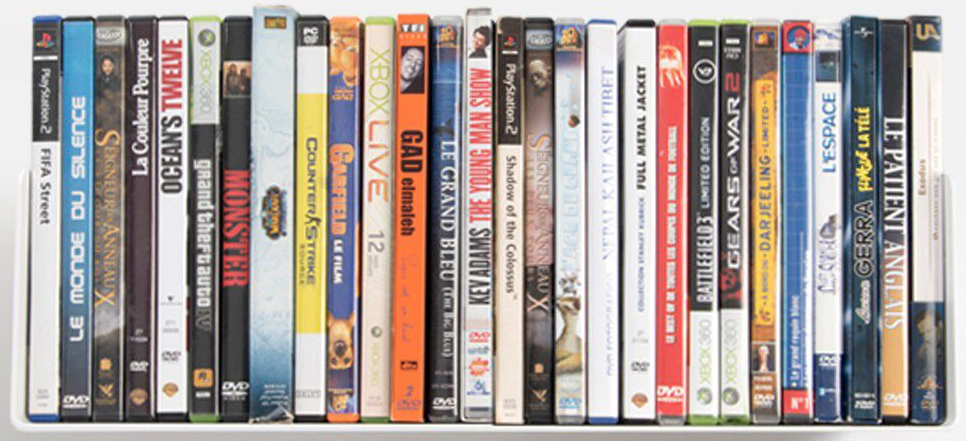
\includegraphics[width=\textwidth,height=3cm,keepaspectratio]{images/find_my_disk.png}
	\end{center}
	
	\item \textbf{Disks:} A \textit{disk} can be the encasing of any CD, DVD, BluRays, audio cassettes, LP, etc. These objects will not be available for training during setup days, although samples can be provided.
	\item \textbf{Test start:} The robot moves to the area near the bookcase where the items are.
\end{enumerate}

\begin{enumerate}
	\item \textbf{Object manipulation:} All manipulation will be performed by the human operator under the supervision of the robot.

	\item \textbf{Object description and dialogs:} The robot shall provide accurate visual descriptions of the discs in the shelf, and those that are presented to it until the desired object is found. The robot can also lead the interaction by asking relevant questions (e.g.~\textit{what's the cover color?} or \textit{what's the title/author?}), so it can look in the spines and covers as necessary.\\
	It is also acceptable (although not advised), to review each title one by one.

	\item \textbf{Clear area:} The robot may assume that the working area is clear, with no people around making loud noises.
	
% 	\item \textbf{Deus ex Machina:} The scores are reduced if human assistance is received, in particular:
% 	\begin{itemize}[nosep]
% 		\item Human leads the conversation
% 	\end{itemize}

\end{enumerate}

\subsection*{Instructions:}

\subsubsection*{To Referee}

The referee needs to:
\begin{itemize}
	\item Rearrange the disks on the bookcase.
	\item Provide instruction to the operator.
	\item Blindfold the operator.
\end{itemize}

\subsubsection*{To OC}
The OC needs to:
\begin{itemize}[nosep]
	\item \textbf{On setup day}: Provide media samples for practice.
\end{itemize}

% \newpage
\subsection*{Score sheet}

The maximum time for this test is 5 minutes.

\begin{scorelist}
	\scoreheading{Main Goal}
	\scoreitem{1000}{Desired disk is found}

	\scoreheading{Bonus rewards}
	\scoreitem{500}{Provide labeled recorded data}
	\scoreitem{1000}{Help operator to find a second disk}

\end{scorelist}


% Local Variables:
% TeX-master: "Rulebook"
% End:


% Local Variables:
% TeX-master: "Rulebook"
% End:

\newpage
\section{Hand Me That [Party Host]}
\label{test:hand-me-that}
A guest at the party speaks English, but with only a limited vocabulary. The robot will assist them in obtaining things that they gesture for.\\
% Comments: In this tasks each group of items is scored separately. Hence 

%\subsection{Focus}
%Joint attention is a well-studied and important task in Human-Robot Interaction. The goal of this task is to really challenge the teams to perform a hard HRI task.


\noindent \textbf{Main Goal:} The robot identifies (touching or naming) each object at which the operator is pointing at.

\subsection*{Focus}
\emph{Object perception}, \emph{HRI}


% %% %%%%%%%%%%%%%%%%%%%%%%%%%%%%%%%%%%%%%%%%%%%%%%%%%%%%%%
%
% Setup
%
% %% %%%%%%%%%%%%%%%%%%%%%%%%%%%%%%%%%%%%%%%%%%%%%%%%%%%%%%
\subsection*{Setup}
\begin{enumerate}[nosep]
	\item \textbf{Location:} 
	\begin{itemize}[nosep]
		\item This takes place in a room in the \Arena{}.
		\item The robot and the operator stand in a predefined starting location announced beforehand % (OC instructions: announce this 2 hours before the test).
	\end{itemize}
	    \item \textbf{Objects:} 
		\begin{itemize}[nosep] 
		\item \textbf{Groups of Objects: }There are five groups of 2--5 objects randomly placed along the room.
		\item \textbf{Deck:} The referee has a deck of objects to request, one per group, sorted by distance.
		\end{itemize}

\end{enumerate}


% %% %%%%%%%%%%%%%%%%%%%%%%%%%%%%%%%%%%%%%%%%%%%%%%%%%%%%%%
%
% Procedure
%
% %% %%%%%%%%%%%%%%%%%%%%%%%%%%%%%%%%%%%%%%%%%%%%%%%%%%%%%%
\subsection*{Procedure}
\begin{enumerate}[nosep]
	\item For each group of objects, the robot asks the operator: \emph{What do you need?}.  % We rule out natural language interaction
		\item The operator walks near to the object and points at it.
		\item The robot asks as many questions as necessary. 
		\item The operator replies to each question (most likely with \emph{yes}, \emph{no}, \emph{I don't know}, single word, etc).
		\\\textbf{Remark:} The operator does not know the name of the object.
\end{enumerate}


% %% %%%%%%%%%%%%%%%%%%%%%%%%%%%%%%%%%%%%%%%%%%%%%%%%%%%%%%
%
% Additional Rules
%
% %% %%%%%%%%%%%%%%%%%%%%%%%%%%%%%%%%%%%%%%%%%%%%%%%%%%%%%%
\subsection*{Additional rules and remarks}
\begin{enumerate}[nosep]
	\item \textbf{Keep going:} The robot should keep trying to determine the referred object until they score or run out of time.

	\item \textbf{Skipping groups:} The robot may say \emph{Pass} or \emph{I give up} to try with the next object.

	\item \textbf{Incorrect guesses:} Incorrect guesses reduce the value of the correct guess the first two times. Guessing correctly on the third or fourth attempt is worth 100 points. After the fourth guess is worth no points.

	\item\textbf{Colors and categories:} Asking for the color or category of a pointed object applies a penalty of 400 points for that particular object.

	\item\textbf{Uneducated operator:} The referee may instruct the operator to answer \emph{I don't understand} or \emph{I don't know} if the robot asks complex questions or is attempting blind guessing.

	\item \textbf{Groups of Objects:} A group consists of 2--5 random standard objects (see~\refsec{rule:scenario_objects}), separated one from another. They can be in a close proximity but not touching.
	The average distance between the starting position and each group ranges between 50cm and 150cm.

\end{enumerate}

\subsection*{Instructions:}

\subsubsection*{To Referee}

The referee needs to:
\begin{itemize}[nosep]
	\item Rearrange and mix groups between runs.
	\item Verify that the operator is pointing at the right item.
\end{itemize}

\subsubsection*{To OC}
The OC needs to:
\begin{itemize}[nosep]
	\item \textbf{On setup day}: Announce the starting position of the robot.
\end{itemize}



\subsection*{Score sheet}

The maximum time for this test is 10 minutes.

\begin{scorelist}
	\scoreheading{Communicating}
	\scoreitem[5]{500}{Correctly determine an item on the first attempt}
	\penaltyitem[5]{-200}{Correctly determine an item on the second attempt}
	\penaltyitem[5]{-400}{Correctly determine an item on a subsequent attempt}
	\penaltyitem[5]{-150}{Asking 1 clarifying question.}
	\penaltyitem[5]{-300}{Asking 2 clarifying questions.}
	\penaltyitem[5]{-450}{Asking 3 clarifying questions.}

	% No longer necessary, computes automatically
	% \setTotalScore{1000}
\end{scorelist}


% Local Variables:
% TeX-master: "Rulebook"
% End:


% Local Variables:
% TeX-master: "Rulebook"
% End:

\newpage
\section{Set the Table [Housekeeper]}
\label{test:set-the-table}
The robot has to set the table for dinner for one person.

% \subsection*{Focus}
% This test focuses on object perception, manipulation, and planning.

\noindent \textbf{Main Goal:} Neatly lay tableware and cutlery on the dining table (5 objects).

\noindent \textbf{Optional goals:}
\begin{enumerate}[nosep]
	\item Picking all utensils from the cupboard drawer
	\item Closing the cupboard drawer
	\item Laying a place mat first
\end{enumerate}


\subsection*{Setup}
\begin{itemize}[nosep]
	\item \textbf{Locations:} This test takes place in the \Arena{}, in a room with a table and a cupboard.
	\item \textbf{Furniture:}
		\begin{itemize}
		 \item Chairs may be placed around the table and will not be removed.
		 \item The cupboard doors and drawers are initially closed.
		\end{itemize}
	\item \textbf{Objects}: 
	\begin{itemize}
		 \item 	The objects used in this test can be found in the cupboard, not in their predefined locations.
		 \item The following objects will be available in the cupboard:
		 \begin{itemize}
			\item\textit{Silverware}: Any two different objects (fork, knife, or spoon).
			\item\textit{Tableware}: A dish and any other object (bowl, cup, or mug).
			\item\textit{Napkin}: A cloth or paper napkin.
			\item\textit{Place mat}: A place mat will be at the bottom of all the object in the cupboard.
		 \end{itemize}
		 
		\end{itemize}
\end{itemize}

% %% %%%%%%%%%%%%%%%%%%%%%%%%%%%%%%%%%%%%%%%%%%%%%%%%%%%%%%
% Procedure
% %% %%%%%%%%%%%%%%%%%%%%%%%%%%%%%%%%%%%%%%%%%%%%%%%%%%%%%%
\subsection*{Procedure}
\begin{enumerate}[nosep]

	\item \textbf{Open cupboard door:} The robot goes to the cupboard and opens the door.
	\item \textbf{Table setup:} The robot picks up five objects from the cupboard, and sets them on the table according to the following placement: 
		\begin{itemize}[nosep]
		 \item Knife and spoon must be placed to the right of the plate.
		 \item The mug or cup must be placed in front of the cutlery.
		 \item Fork and napkin must be placed to the left of the plate.
		 \item The bowl must be stacked on top of the plate.
		\end{itemize}

\end{enumerate}



\subsection*{Additional rules and remarks}
\begin{enumerate}[nosep]
	\item \textbf{Safe placing:} Objects must be placed with care. It must be clear that the robot is trying to place the object, not throwing or dropping it.

	\item \textbf{Deus ex Machina:} Score reductions are applied for requesting the following forms of human assistance:
	\begin{itemize}[nosep]
		\item \textbf{Handover:} Handing over an object.
		
		\item \textbf{Showing objects:} Pointing, or telling to the robot where an object is or where to place it.

	\end{itemize}

	\item \textbf{Cupboard drawers:} If a drawer is available near the cupboard, the team can decide to start the task with the cutlery in the drawer. The team can choose between having the robot open the cupboard door or the drawer, with the referee opening the other one.

\end{enumerate}

\subsection*{Referee instructions}

The referee needs to
\begin{itemize}
	\item Remove all objects from the table
	\item Place objects in their starting position (in the drawer or in the cupboard)
	\item Close the door or drawer, depending on which one the robot is going to attempt to open.
\end{itemize}

\subsection*{OC instructions}
During \SetupDays
\begin{itemize}
	\item Provide official cutlery and tableware for training.
\end{itemize}

% \newpage
\subsection*{Score sheet}
The maximum time for this test is 10 minutes.

\begin{scorelist}
	\scoreheading{Main Goal}
	\scoreitem{100}{Open the drawer or cupboard door}
	\scoreitem[2]{50}{Pick up plate and cup}
	\scoreitem[3]{150}{Pick up knife, spoon, and fork}
	\scoreitem{50}{Pick up napkin}
	\scoreitem[5]{100}{Correctly place each item}
	
	\penaltyitem[5]{25}{Pointing at object}
	\penaltyitem[5]{50}{Pointing at destination}

	\scoreheading{Bonus rewards}
	\scoreitem{500}{Layplace mat before objects}
	\scoreitem{250}{Placing all objects correctly}
	\scoreitem{50}{Closing the door or drawer}

	%\setTotalScore{1000}
\end{scorelist}


% Local Variables:
% TeX-master: "Rulebook"
% End:


% Local Variables:
% TeX-master: "Rulebook"
% End:


\newpage
\section{Stickler for the Rules [Party Host]}
\label{test:stickler-for-the-rules}

\subsection*{Description}
The robot needs to make sure the house rules are followed.

\textbf{Main goal:}
Identify party guests breaking the house rules, politely clarify to the guest what to do and confirm that the guest is following the rule.

\textbf{Optional goal:}
Politely clarify to the guest what rule is being broken.


\subsection*{Focus}
This task focuses on
\textit{Object perception},
\textit{Human perception},
\textit{Action recognition} and
\textit{Verbal interaction}.

\subsection*{Setup}
\begin{itemize}[nosep]	
	\item \textbf{Locations:} 
	\begin{itemize}
		\item This task takes place inside the \Arena{}.
		\item The robot starts at a predefined location in the living room.
		\item There are a forbidden room in the house.
	\end{itemize}	 
	\item \textbf{People:} 
	\begin{itemize}
		\item There are at least 5 party guests inside the \Arena{}.
		\item Four of the guests are breaking rules.
		\item Guests may not follow the robot's instructions.
	\end{itemize}
	\item \textbf{Furniture:} All furniture are in their predefined locations.
	\item \textbf{Objects:} All objects are in their predefined locations.
\end{itemize}

\subsection*{Procedure}
	\begin{enumerate}[nosep]
		\item
	\end{enumerate}


\subsection*{Additional rules and remarks}
\begin{itemize}[nosep]
	\item \textbf{House Rules:}
	\begin{enumerate}[nosep]
		\item \textit{No shoes inside the house.}\\
		\textbf{Policy:} All guests have to take off their shoes at the entrance.\\
		\textbf{Action:} Take the guest to the entrance and verify she takes off her shoes.
	
		\item \textit{Rorbidden room}\\
		\textbf{Policy:} No guests are allowed in the \emph{Black Room}.
		\textbf{Action:} Take the offender with other party guests and verify she doesn't enter back.
	
		\item \textit{No littering}\\
		\textbf{Policy:} Guests are not allowed to leave garbage on the floor.
		\textbf{Action:} Make the (closest) offender to pick up the garbage and throw it into the bin.
	
		\item \textit{Compulsory hydration}\\
		\textbf{Policy:} All guests must have a drink in hand at all times.\\
		\textbf{Action:} Take the guest to the kitchen/bar and make sure she grabs a drink.
	\end{enumerate}
\end{itemize}

\subsection*{Instructions}
\subsubsection*{Referee}

The referee needs to
\begin{itemize}
	\item Instruct party guests on which rules to break.
	\item Assign each party guest a drink.
\end{itemize}

\subsubsection*{OC}
2h before test:
\begin{itemize}
	\item Select and announce the robot start location.
	\item Select and announce which room is forbidden.
\end{itemize}

% \newpage
\subsection*{Score sheet}

The maximum time for this test is 10 minutes.

\begin{scorelist}
	\scoreheading{Main Goal}
	\scoreitem[3]{250}{Recognize guests breaking rules and ask them to stop}
	\scoreheading{Bonus Goal}
	\scoreitem[3]{250}{Control if guests stop breaking rules}
\end{scorelist}


% Local Variables:
% TeX-master: "Rulebook"
% End:


% Local Variables:
% TeX-master: "Rulebook"
% End:


\newpage
\section{Where is This? [Party Host]}
The robot has to explain to people where they can find places in the arena.


\subsection{Main Goal}
People will approach the robot and ask where they can find a location in the arena (i.e. "Where is the TV?"). The robot has to either accurately describe the location from the other persons perspective (i.e. "It is to your right..." or "Turn around and go towards...") or guide the person there.

\noindent\textbf{Reward:} 1000pts (100pts per described location).

\subsection{Bonus rewards}
\begin{enumerate}[nosep]
	\item Recognize when a person returns and help them again. 250 (50 pts each).
\end{enumerate}

\subsection{Setup}
\begin{itemize}[nosep]
	\item \textbf{Locations:} All predefined locations inside the arena.
\end{itemize}

\subsection{Additional rules and remarks}
\begin{enumerate}[nosep]
	 \item Instead of describing the location the robot may guide the person there but this will probably take more time.
	 \item Five of the guests will come back later to ask for further instructions. I.e. "Where is the TV?" - "It is in the room behind you in the rightmost corner" - later - "I only found the sofa" - "The TV is to the left of the sofa". The robot has to remember where the person wanted to go in the first place. If the robot can give advanced instructions based on the location that the person found the bonus points are awarded.
\end{enumerate}

\subsection{Referee instructions}
The referee needs to
\begin{itemize}
	\item Assign locations to persons.
	\item Assign follow up questions to five persons.
\end{itemize}

\subsection{OC instructions}
2 hours before the test:
\begin{itemize}
	\item Announce where the robot has to wait for people to approach.
\end{itemize}

\newpage
\subsection{Score sheet}

The maximum time for this test is 10 minutes.

\begin{scorelist}
	\scoreheading{Main Goal}
	\scoreitem[3]{100}{Describe and show the requested location accurately}
	\scoreitem[3]{50}{Using naive operator}
	\penaltyitem[3]{50}{Using custom operator}

	\scoreheading{Bonus rewards}
	\scoreitem[3]{200}{Guide the 4th guest on}
	\scoreitem[3]{50}{Using naive operator}
	\penaltyitem[3]{100}{Using custom operator}
	\scoreitem[3]{100}{Recognize a person and give further instructions.}
	\scoreitem[6]{100}{Provide audio recording and transcripts}
\end{scorelist}

% Local Variables:
% TeX-master: "Rulebook"
% End:



\chapter{Finals}

The competition ends with the Finals on the last day, where the two teams with the highest total score compete.
The \iterm{Finals} are conducted as a final themed demonstration.

%To avoid logistical issues during the last day of the competition, the \iterm{Finals} are divided into two sets of demonstrations: the Bronze Competition and the RoboCup @Home Grand Finale.
%The Bronze Competition is a set of demonstrations that are carried out before the RoboCup @home Grand Finale. Here, all the leagues run in parallel, with the fourth and third highest scored teams competing for the bronze.
%Finally, the two teams with the highest score in each League present their demonstrations in a serialized manner during the RoboCup @Home Grand Finale.

Even though each league has its own first, second and third place, the \iterm{Finals} are meant to show the best of all leagues to the jury members as well as the audience and, thus, warrants a single schedule slot.

\section{Structure and Theme}

The \iterm{Finals} are a demonstration of achieving an objective that is pre-selected by the TC/EC. These objectives are chosen as a type of yearly theme of the competition, and to provide a baseline for the juries (not to mention the audience) to state which team is the winner.

The objectives for each league for this year are:

\begin{itemize}
    \item \emph{OPL/DSPL}: The robot helps a person that has had a small accident in their home.
    \item \emph{SSPL}: The robot monitors a person while they are going about their day and reacts appropriately if it notices any unusual events.
\end{itemize}


The teams are expected to provide a demonstration that is telling a story which includes achieving the objective. The teams can choose freely how to achieve it, which includes choosing the participants, what items to use, the methods employed, etc. The juries, as explained later, will reward elegance and difficulty.

As it can be seen, the objectives are open enough that a story can be told around them which can include additional objectives that the team wants their robot to also solve. Thus, the teams are welcome to include in their demonstration any additional tasks to be solved, which can serve as a type of forum where they can present their own research. The innovation and success of these tasks will also be used as part of the score (as it is described later). In this regard, it is expected that teams present the scientific and technical contributions they submitted in both \iterm{team description paper} and the \iterm{RoboCup\char64Home Wiki}.

In addition, teams may provide a printed document to the jury (max 1 page) that summarizes the demonstrated robot capabilities and contributions. However, teams are discouraged to provide any material that would distract from their demonstration.

Story-telling is an important factor, so it is recommended to spend the least amount of time using the microphone to explain the demonstration and let the demonstration speak for itself.


\section{Evaluating Juries for Final Demonstrations}
The \iterm{Finals} are evaluated by two juries, here described.

\begin{enumerate}
\item\textbf{League-internal jury:} The league-internal jury is formed by the Executive Committee. The evaluation of the league-internal jury is based on the following criteria:
  \begin{compactenum}
  \item Efficacy/elegance of the solution
  \item Innovation/contribution to the league of the additional tasks solved
  \item Difficulty of the overall demonstration
  \end{compactenum}

\item \textbf{League-external jury:} The league-external jury consists of people not being involved in the RoboCup@Home league, but having a related background (not necessarily robotics). They are appointed by the Executive Committee. The evaluation of the league-external jury is based on the following criteria:
  \begin{compactenum}
  \item Originality and presentation (story-telling is to be rewarded)
  \item Relevance/usefulness to everyday life
  \item Elegance/success of overall demonstration
  \end{compactenum}
\end{enumerate}

\section{Scoring}
The final score and ranking are determined by the jury evaluations and by the previous performance (in Stages I and II) of the team, in the following manner:

\begin{enumerate}
  \item The influence of the league-internal jury to the final ranking is \SI{25}{\percent}.
  \item The influence of the league-external jury to the final ranking is \SI{25}{\percent}.
  \item The influence of the total sum of points scored by the team in Stage I and II is \SI{50}{\percent}.
\end{enumerate}

These demonstrations are carried out in a serialized fashion, one League performing after another in one \Arena{}.


\subsection{Task}
The procedure for the demonstration and the timing of slots is as follows:
\OpenDemonstrationTask{ten}{five}

\OpenDemonstrationChanges

%% %%%%%%%%%%%%%%%%%%%%%%%%
\section{Final Ranking and Winner}

There will be an award for 1st, 2nd and 3rd place of each league.

The winner of the competition is the team that gets the highest ranking in the \iterm{Finals}.

The second place will be the team that got the second-highest ranking in the \iterm{Finals}.

The third place will be the team with the highest score that did not made it to the \iterm{Finals}.

Additional certificates would be granted if:

\begin{enumerate}
  \item If the number of teams in the league is above 11, a certificate will be awarded to the 4th ranked team.
  \item If the number of teams in the league is above 14, a certificate will be awarded to the 5th ranked team.
\end{enumerate}


% Local Variables:
% TeX-master: "Rulebook"
% End:



\printabx
\printidx

\end{document}
